\section{Multilayer mirror 1}
\subsection{Input beam}
A beam snapshot at 15.165 m from source is shown in Figure \ref{fig:snapshot_ML1}.
\begin{figure}[ht]
\centering
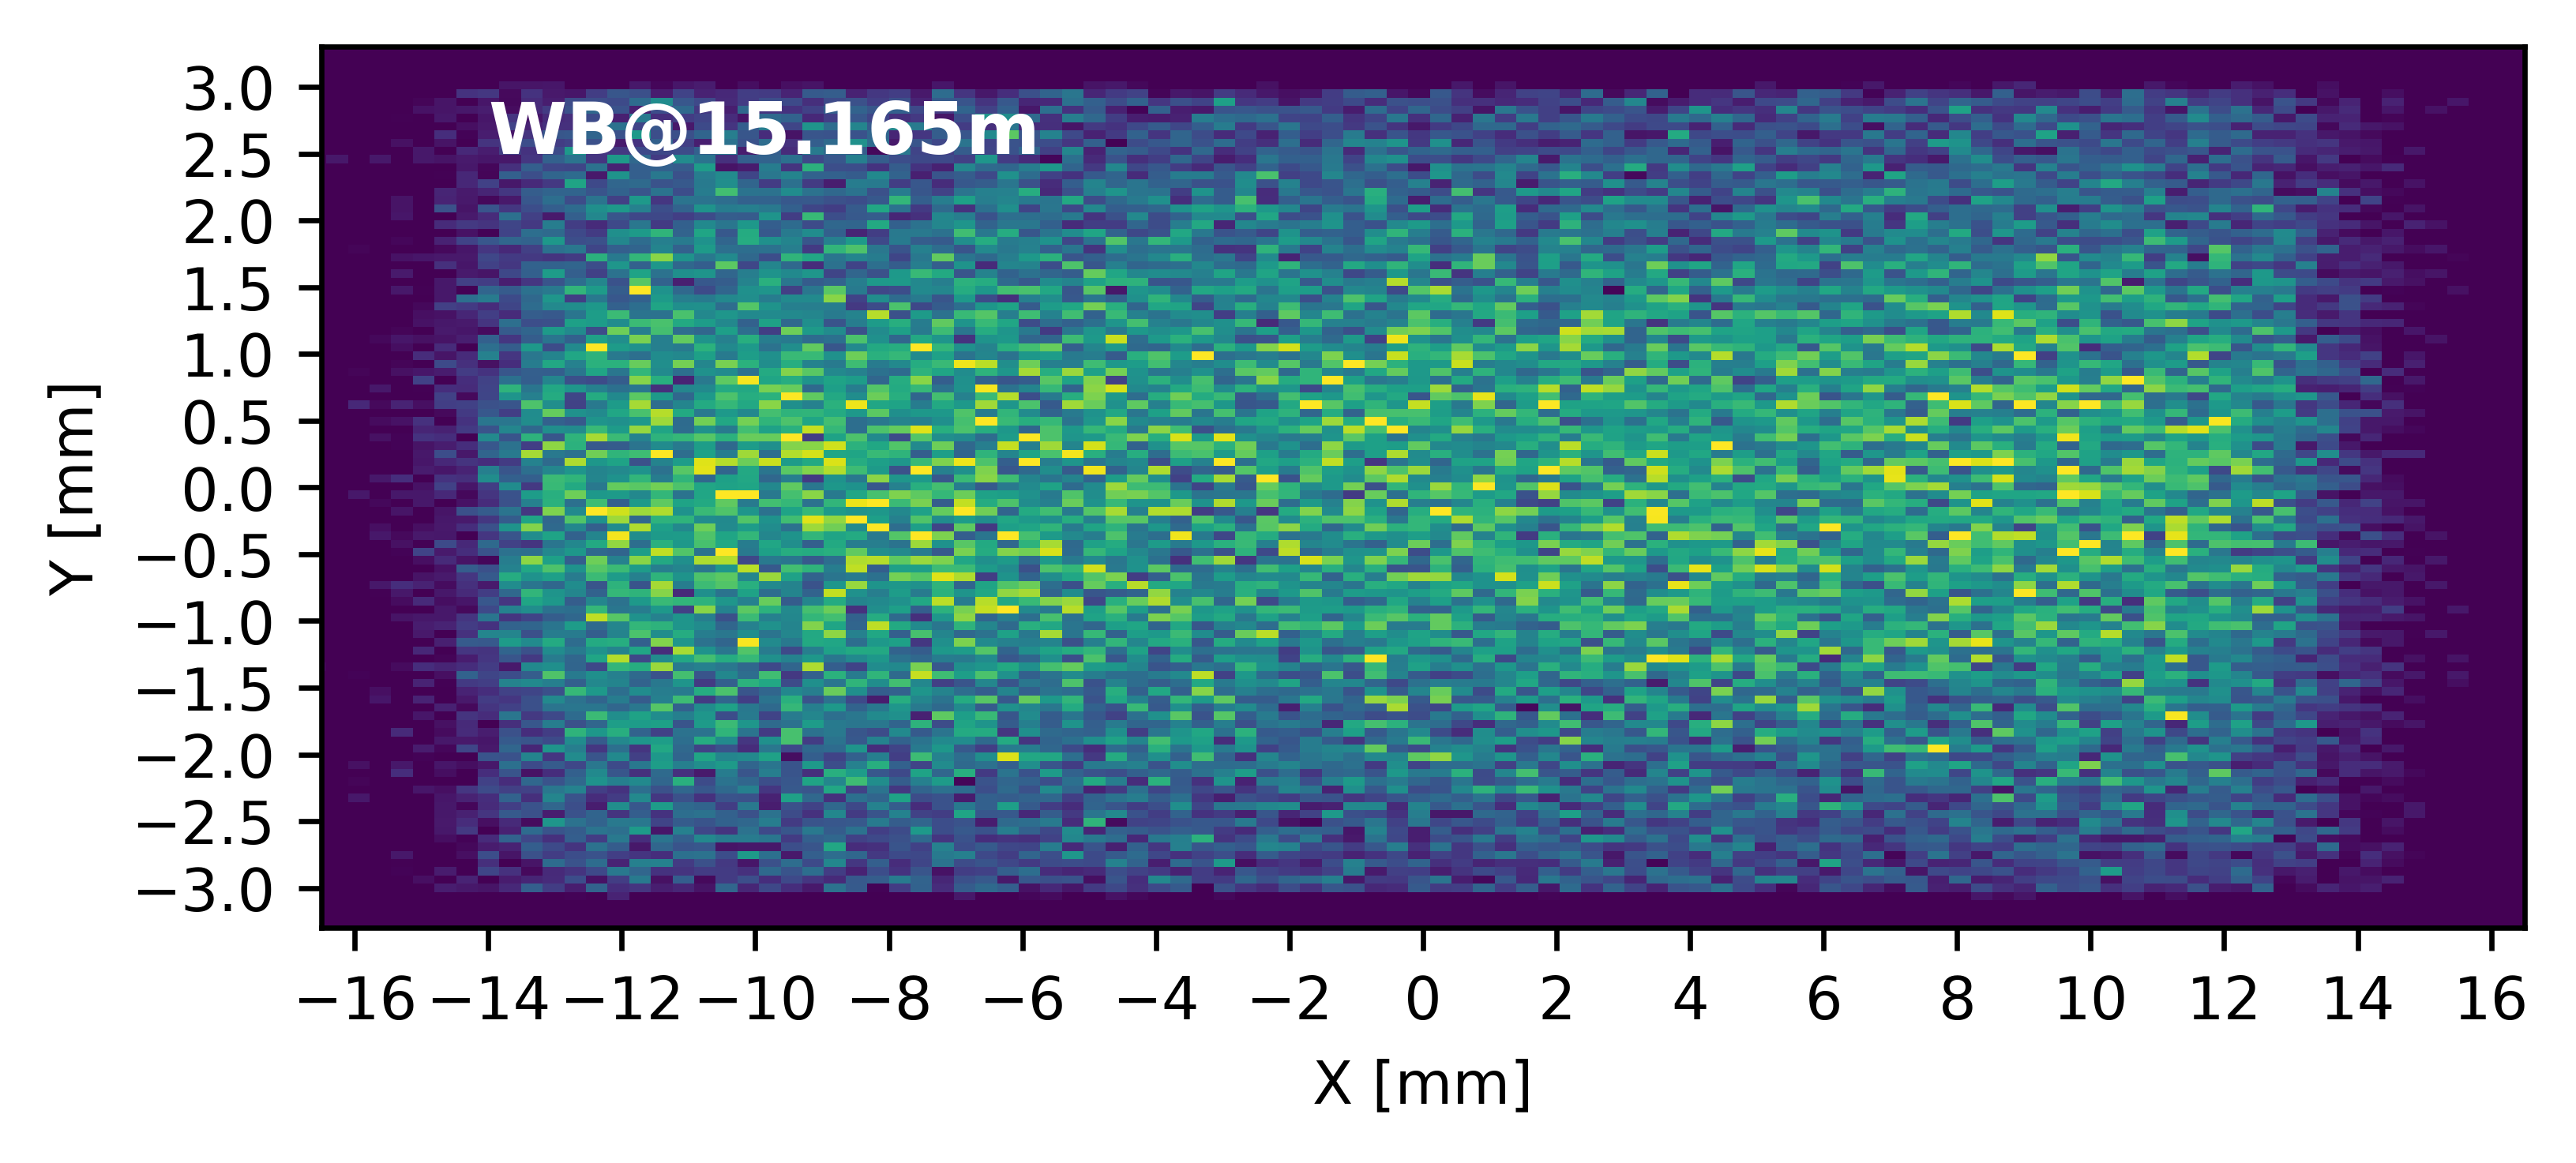
\includegraphics[width=0.8\textwidth]{./../../beam_snapshots/WB_snapshot_15.165.png}
\caption{\label{fig:snapshot_ML1} White beam snapshot at 15.165 m from source (center position of ML1).}
\end{figure}

%%%%%%%%%%%%%%%%%%%%%%%%%%%%%%%%%%%%%%%%%%%%%%%%%%%%%%%%%%%%%%%%%%%%%%%%%%%%%%%%%%%%
\subsection{Substrate design}
The center of the first multilayer mirror of the BEATS DMM is positioned at 15.165 m from the ID photon source. \\
CINEL proposed to increase the ML length to 500 mm. A drawing of the proposed substrate is attached.

%%%%%%%%%%%%%%%%%%%%%%%%%%%%%%%%%%%%%%%%%%%%%%%%%%%%%%%%%%%%%%%%%%%%%%%%%%%%%%%%%%%%
\subsection{Substrates slope error}
For this paragraph a substrate length of 500 mm is considered.

\subsubsection{Raytracing}
\begin{wrapfigure}{r}{0.3\linewidth}
\centering
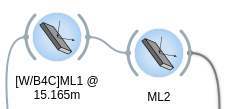
\includegraphics[width=0.3\textwidth]{images/DMM_oasys.png}
\caption{\label{fig:DMM_oasys} Double Multilayer Monochromator in Oasys Shadow.}
\end{wrapfigure}

The double-bounce DMM is modelled with two Shadow Plane Mirror widgets in series (Figure \ref{fig:DMM_oasys}). ML reflectivity is modelled with a Shadow PreMLayer widget as shown in Figure \ref{fig:PreMLayer}. The mirror surface is modified with Surface Error external splines with varying longitudinal slope error (0.1, 0.2, 0.3, 0.4 and 0.5 $\mu rad$ RMS). These modified surfaces (\ref{fig:fractals}) are simulated with the Shadow PreProcessor - Height Profile Simulator widget. The transversal slope error is kept constant at 20 $\mu rad$ RMS and fractal profiles are chosen. 

\begin{figure}  % spans both columns
\begin{subfigure}{0.5\textwidth}
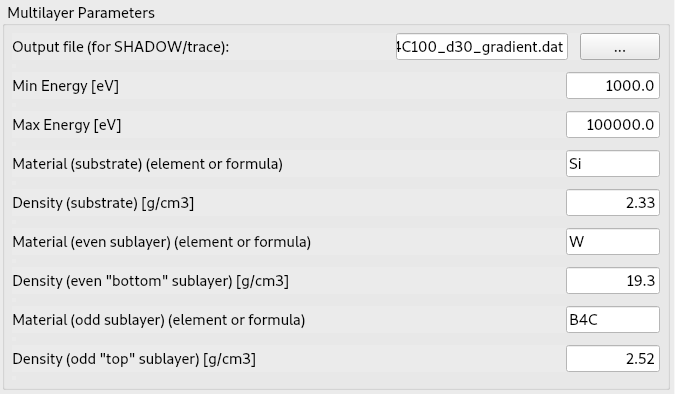
\includegraphics[width=\linewidth]{images/MLspecs_a.png}
\end{subfigure}
\hfill % maximize the horizontal distance between the graphs
\begin{subfigure}{0.5\textwidth}
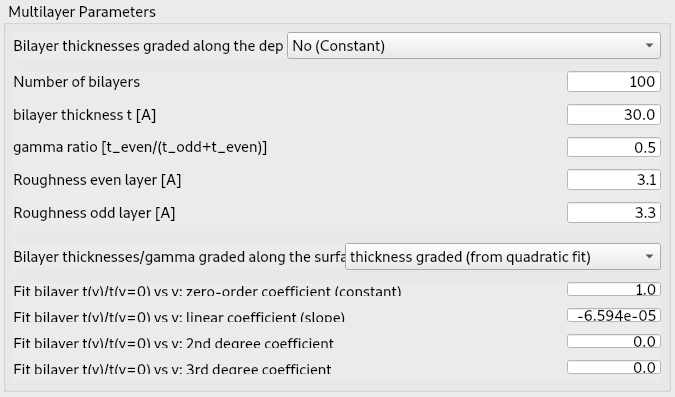
\includegraphics[width=\linewidth]{images/MLspecs_b.png}
\end{subfigure}
\caption{\label{fig:PreMLayer} PreMLayer widget settings in Shadow. }
\end{figure}

\begin{figure}[!htb]
\minipage{0.32\textwidth}
  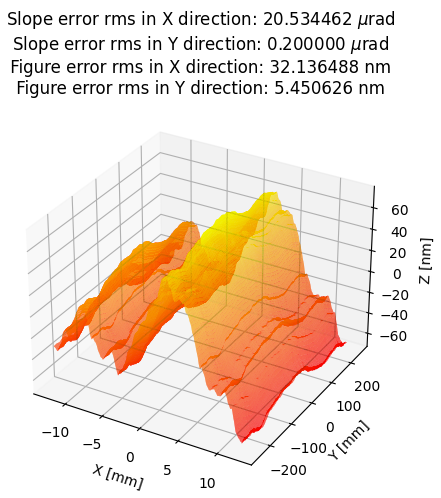
\includegraphics[width=\linewidth]{./../figures/slope_error/surface_error_profile_500x25_02x20urad.png}
  % \caption{A really Awesome Image}\label{fig:awesome_image1}
\endminipage\hfill
\minipage{0.32\textwidth}
  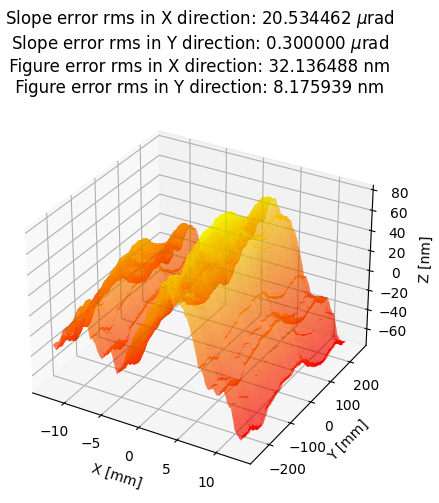
\includegraphics[width=\linewidth]{./../figures/slope_error/surface_error_profile_500x25_03x20urad.png}
  % \caption{A really Awesome Image}\label{fig:awesome_image2}
\endminipage\hfill
\minipage{0.32\textwidth}%
  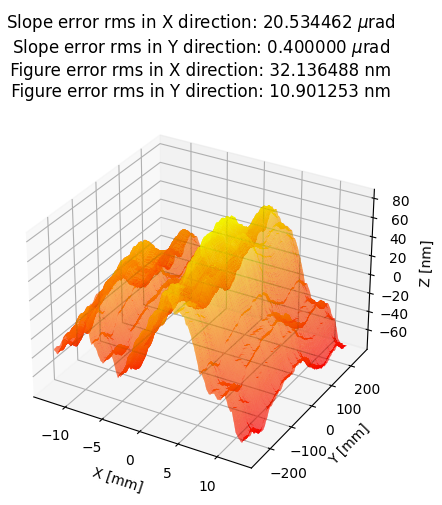
\includegraphics[width=\linewidth]{./../figures/slope_error/surface_error_profile_500x25_04x20urad.png}
  %\caption{A really Awesome Image}\label{fig:awesome_image3}
\endminipage
\caption{\label{fig:fractals} Modified mirror surfaces. }
\end{figure}

%%%%%%%%%%%%%%%%%%%%%%%%%%%%%%%%%%%%%%%%%%%%%%%%%%%%%%%%%%%%%%%%%%%%%%%%%%%%%%%%%%
\clearpage
\subsubsection{0.1 urad}
\begin{figure}[H]
\centering
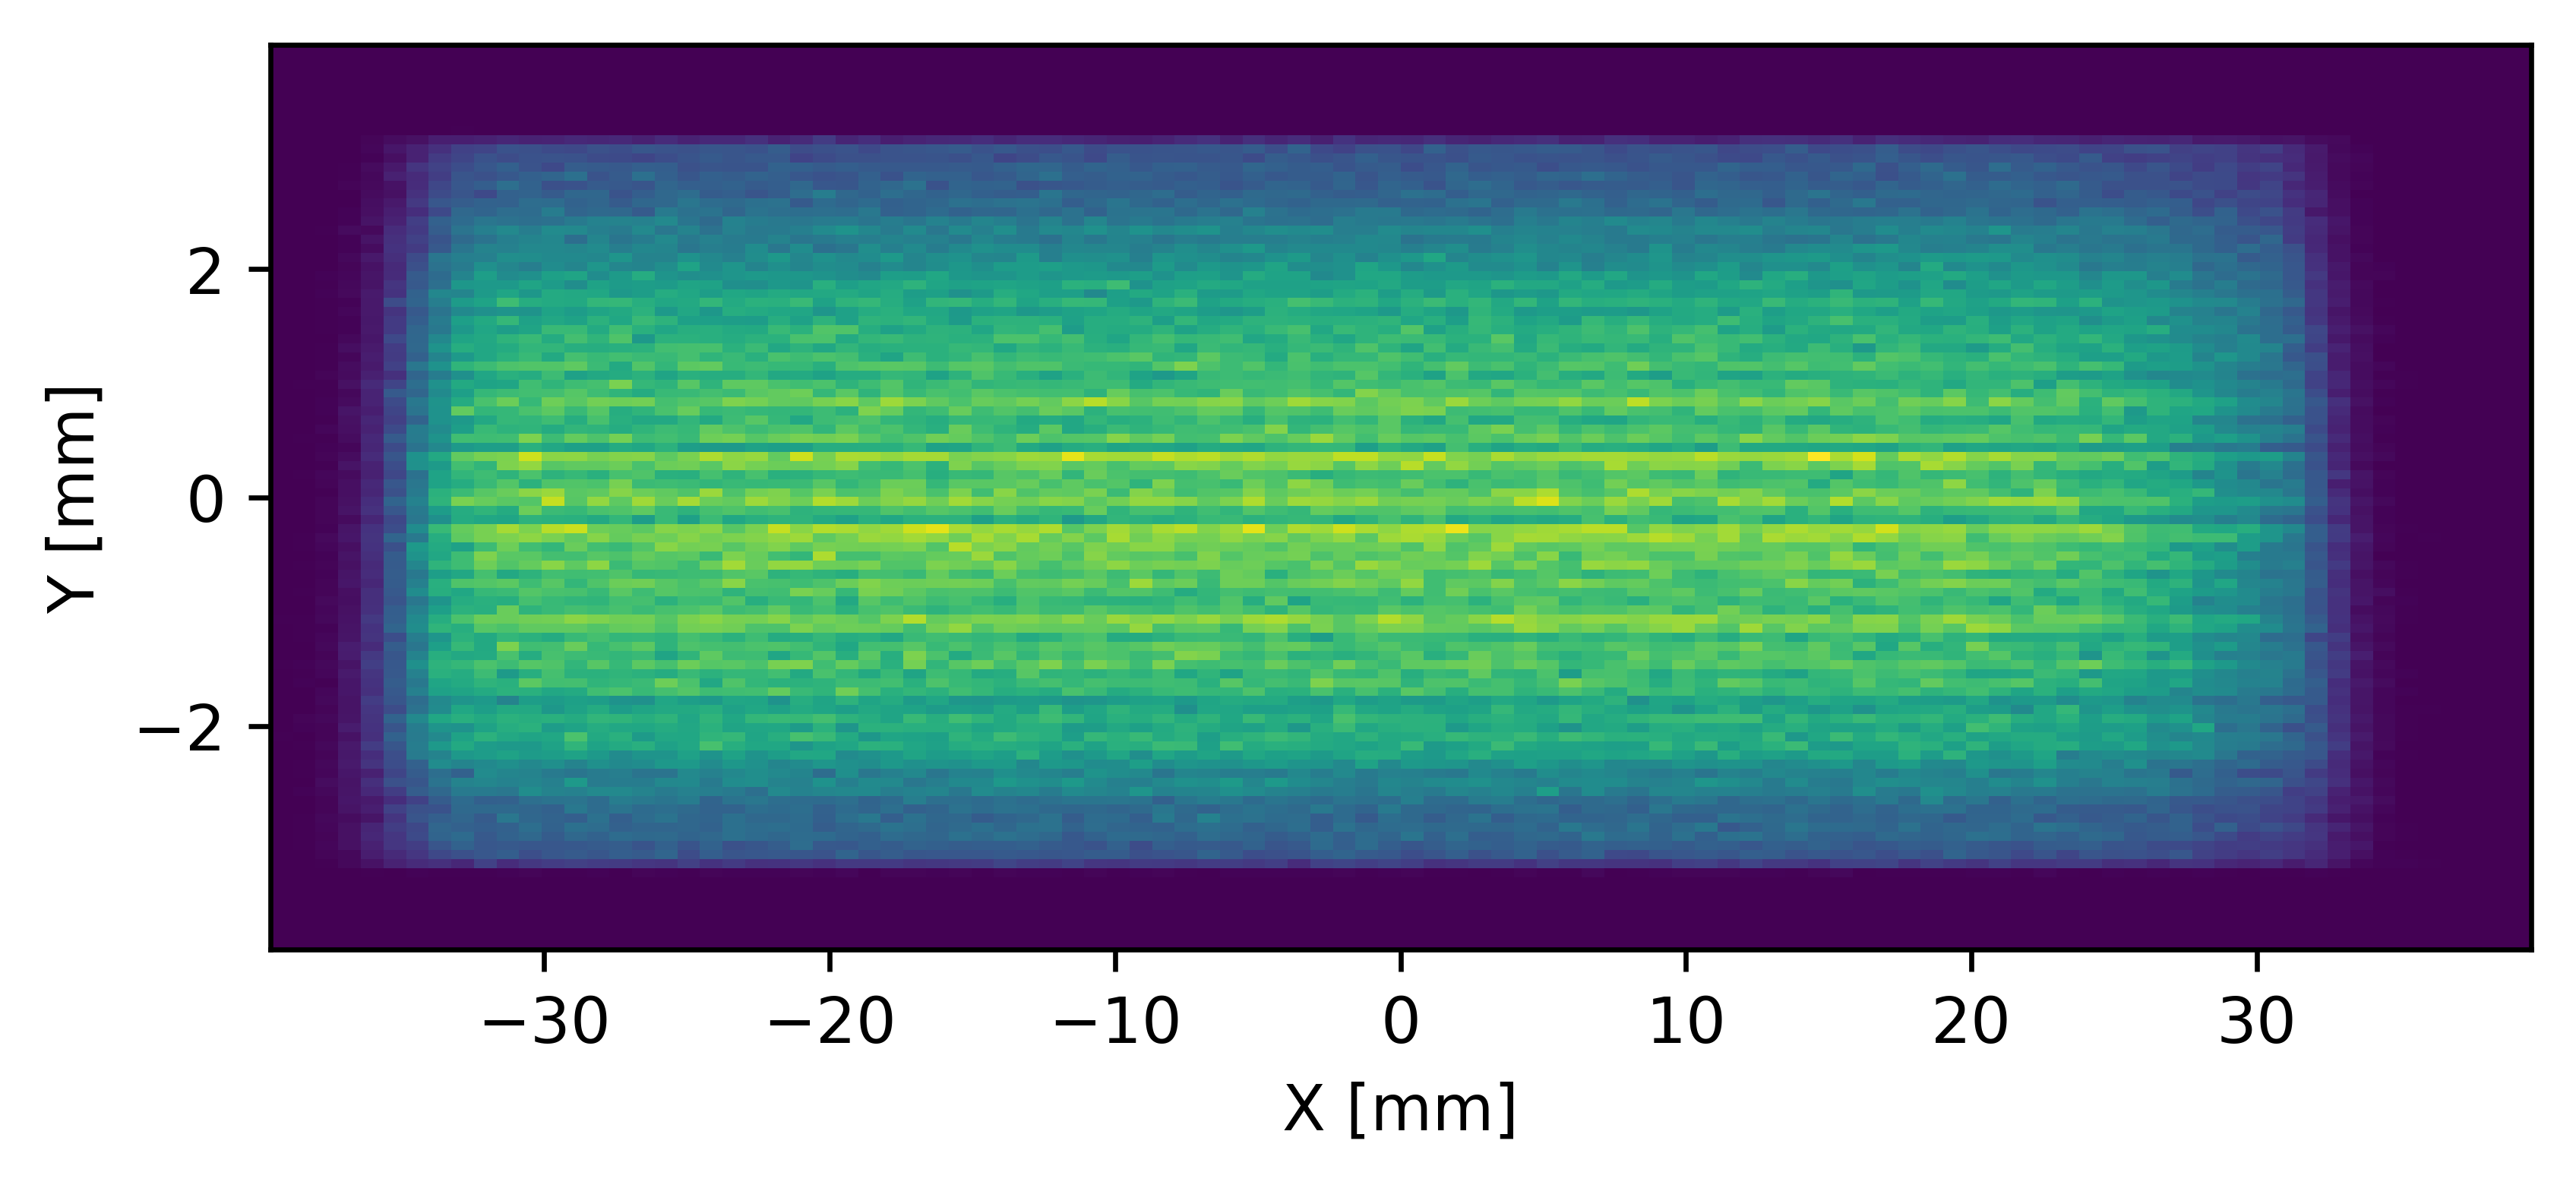
\includegraphics[width=0.9\linewidth]{./../figures/slope_error/WB4C_d30_d-spacing_gradient_45keV_slope_error01urad.png}
\end{figure}

\begin{figure}[H]
\centering
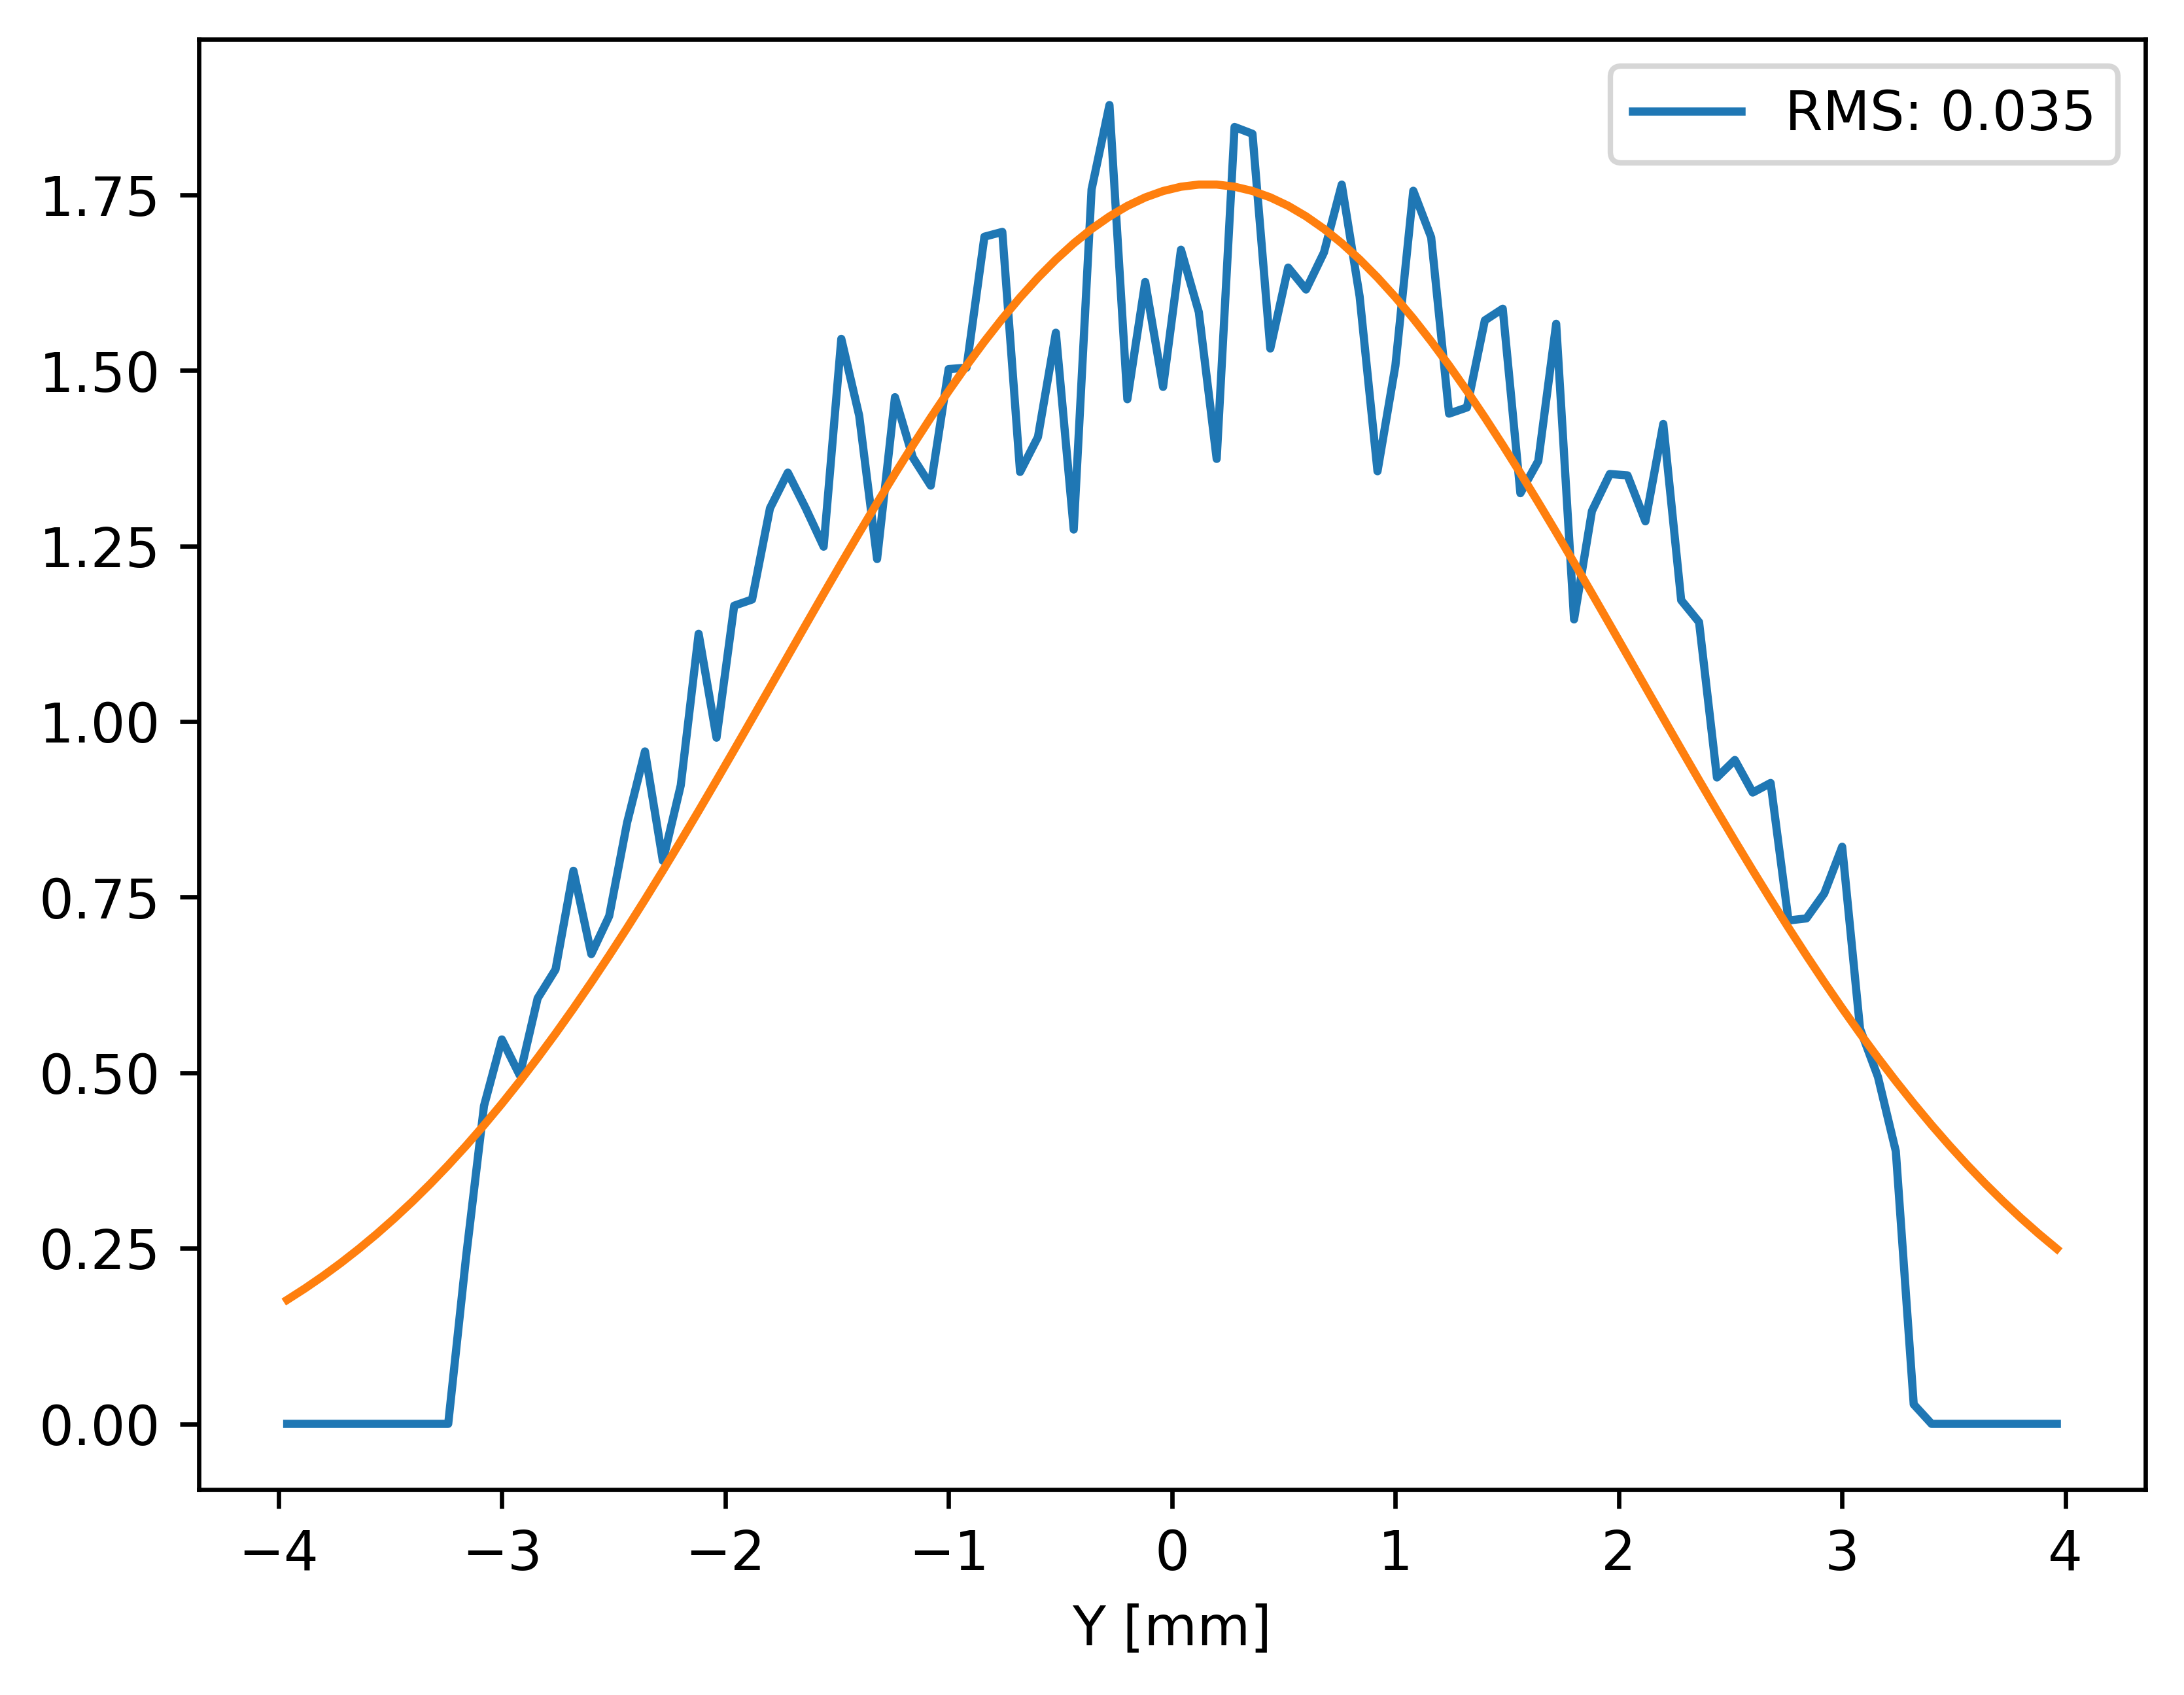
\includegraphics[width=0.9\linewidth]{./../figures/slope_error/WB4C_d30_d-spacing_gradient_45keV_slope_error01urad_Yprofile.png}
\caption{0.1 urad}
\label{fig:01urad}
\end{figure}

%%%%%%%%%%%%%%%%%%%%%%%%%%%%%%%%%%%%%%%%%%%%%%%%%%%%%%%%%%%%%%%%%%%%%%%%%%%%%%%%%%
\clearpage
\subsubsection{0.2 urad}
\begin{figure}[H]
\centering
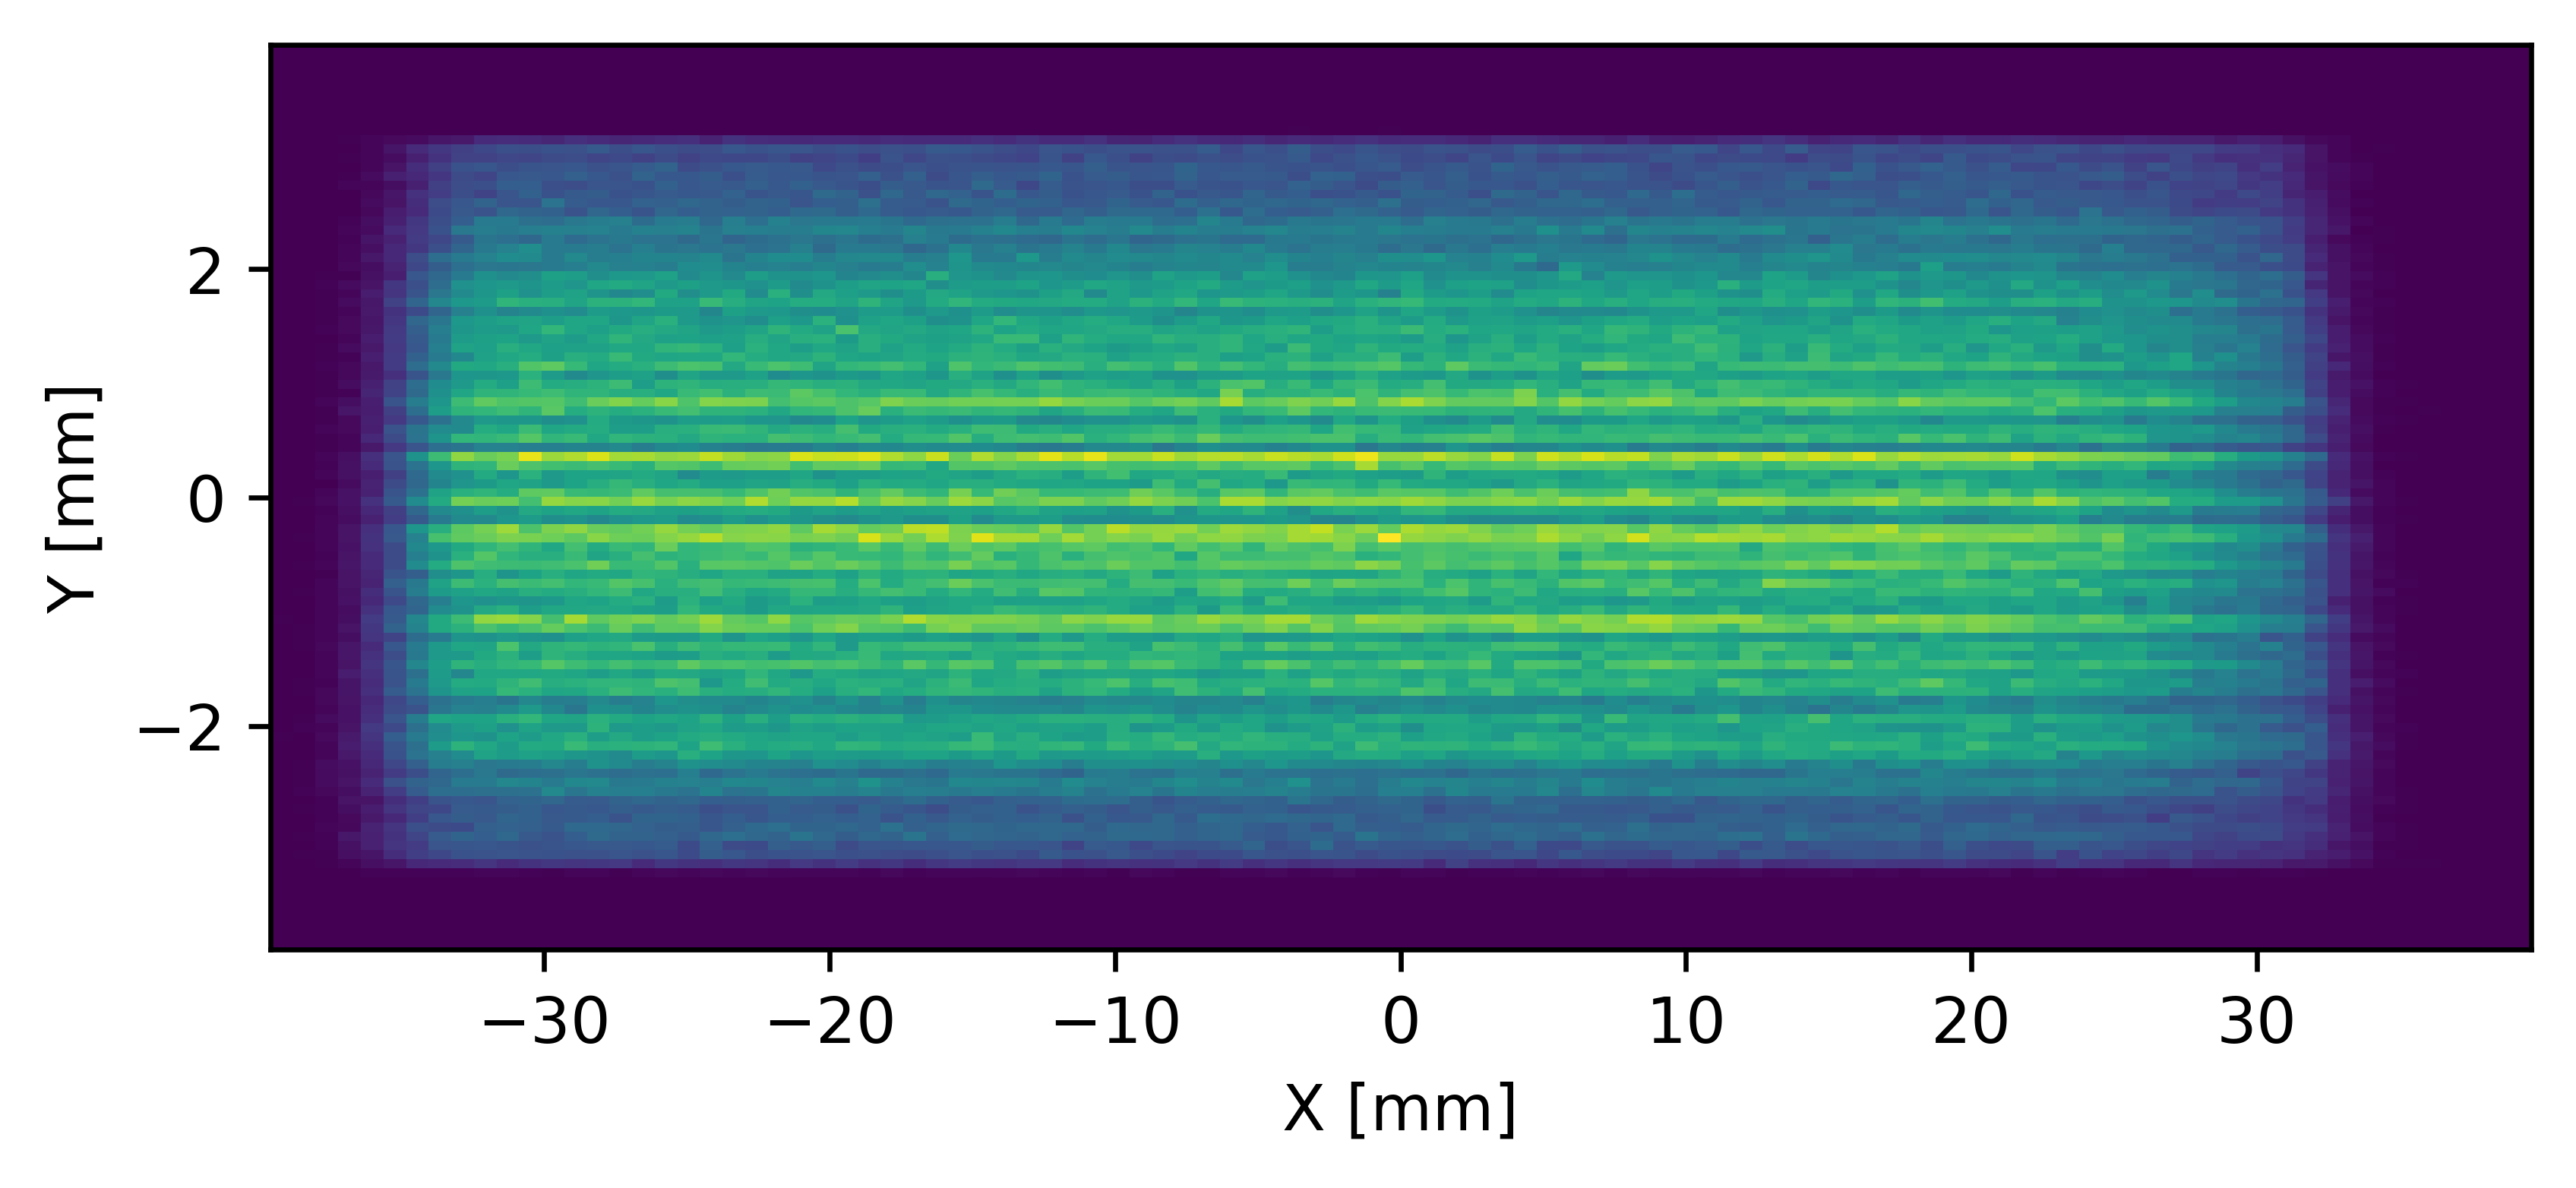
\includegraphics[width=0.9\linewidth]{./../figures/slope_error/WB4C_d30_d-spacing_gradient_45keV_slope_error02urad.png}
\end{figure}

\begin{figure}[H]
\centering
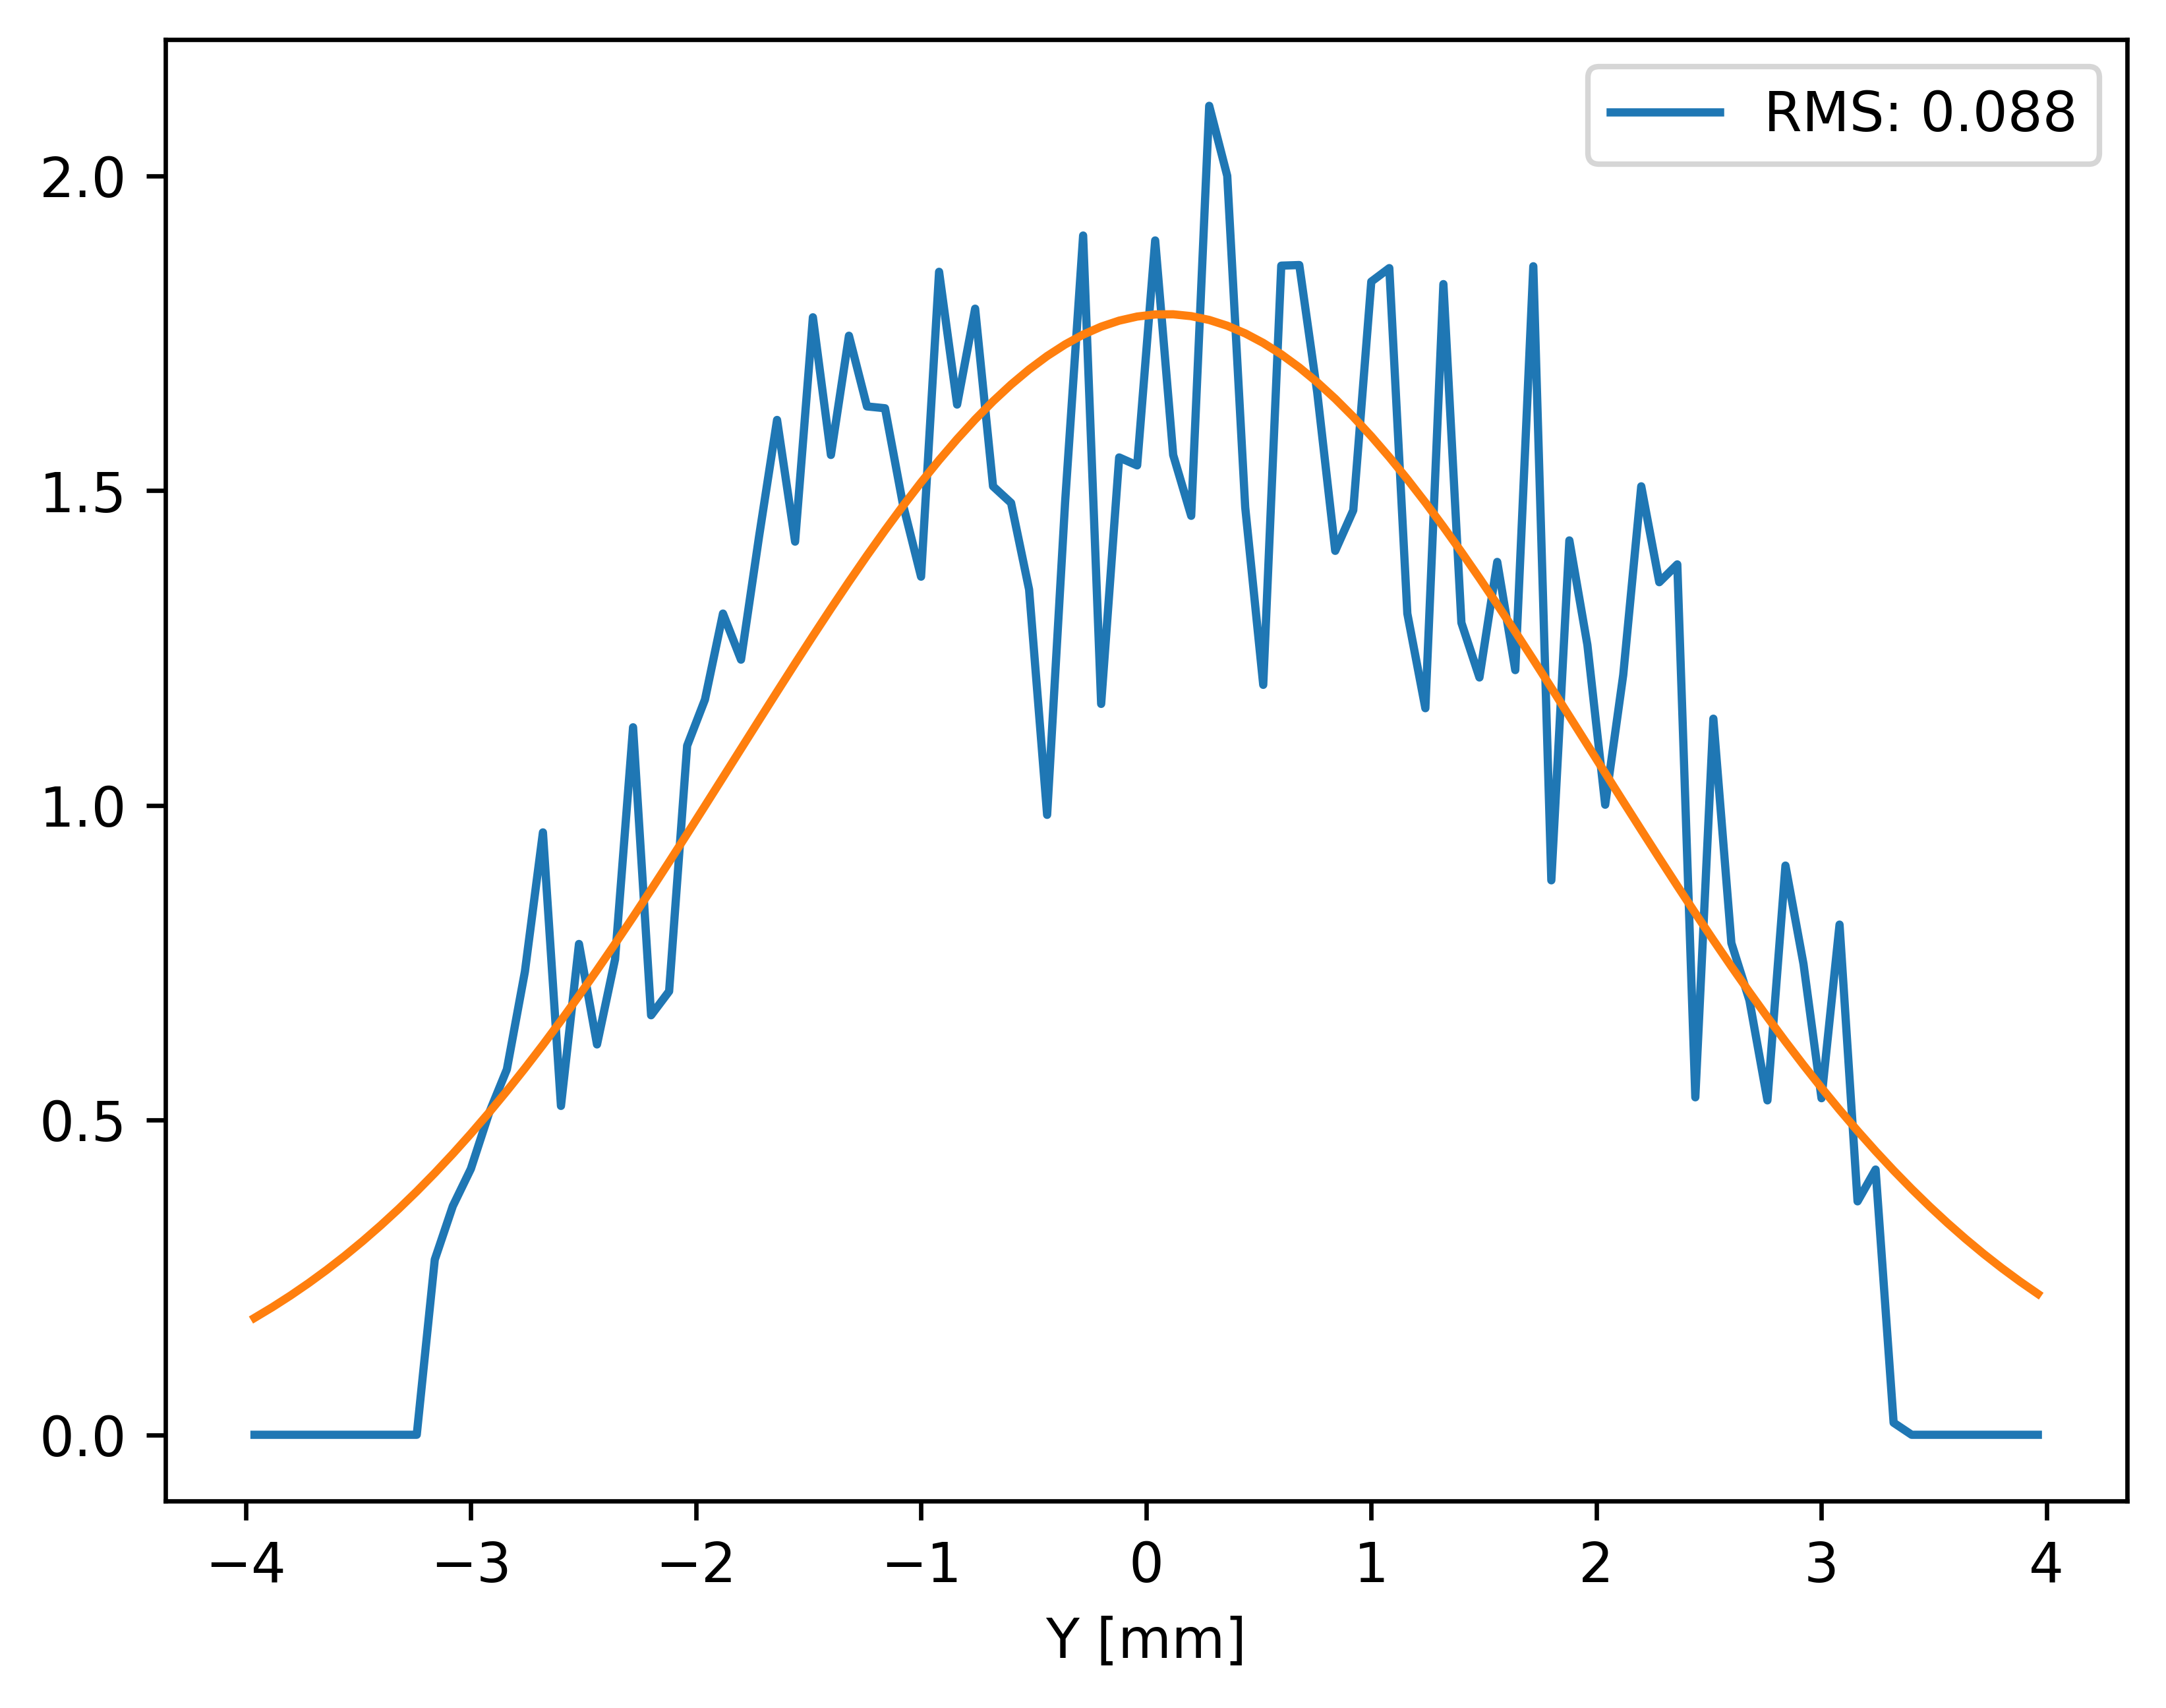
\includegraphics[width=0.9\linewidth]{./../figures/slope_error/WB4C_d30_d-spacing_gradient_45keV_slope_error02urad_Yprofile.png}
\caption{0.2 urad}
\label{fig:02urad}
\end{figure}

%%%%%%%%%%%%%%%%%%%%%%%%%%%%%%%%%%%%%%%%%%%%%%%%%%%%%%%%%%%%%%%%%%%%%%%%%%%%%%%%%%
\clearpage
\subsubsection{0.25 urad}
\begin{figure}[H]
\centering
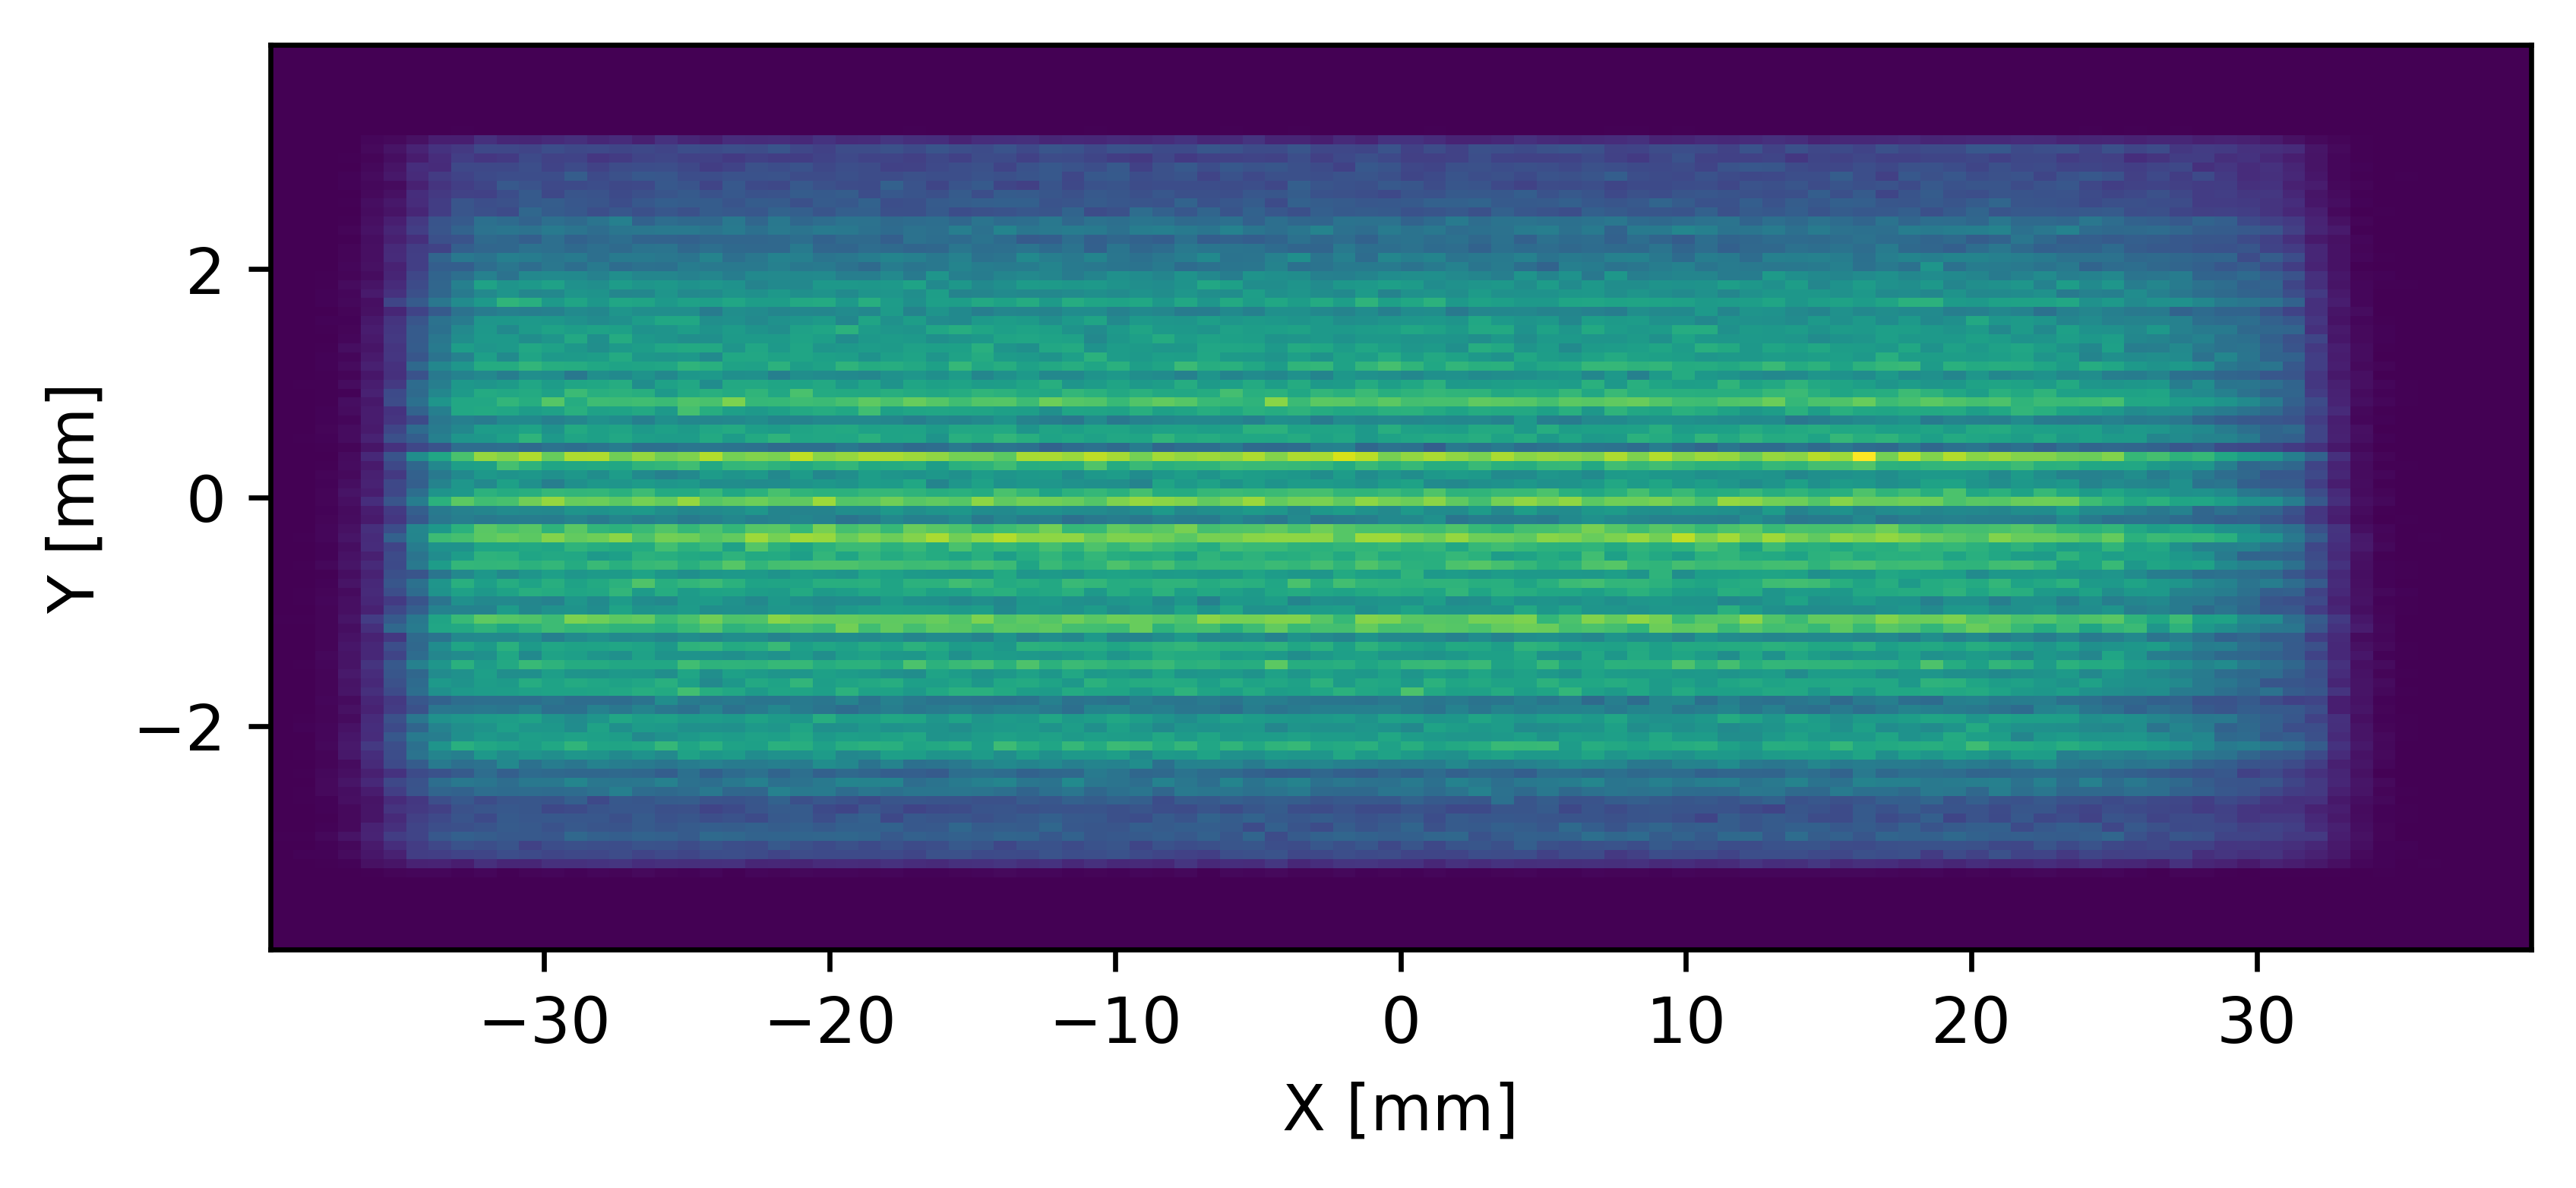
\includegraphics[width=0.9\linewidth]{./../figures/slope_error/WB4C_d30_d-spacing_gradient_45keV_slope_error025urad.png}
\end{figure}

\begin{figure}[H]
\centering
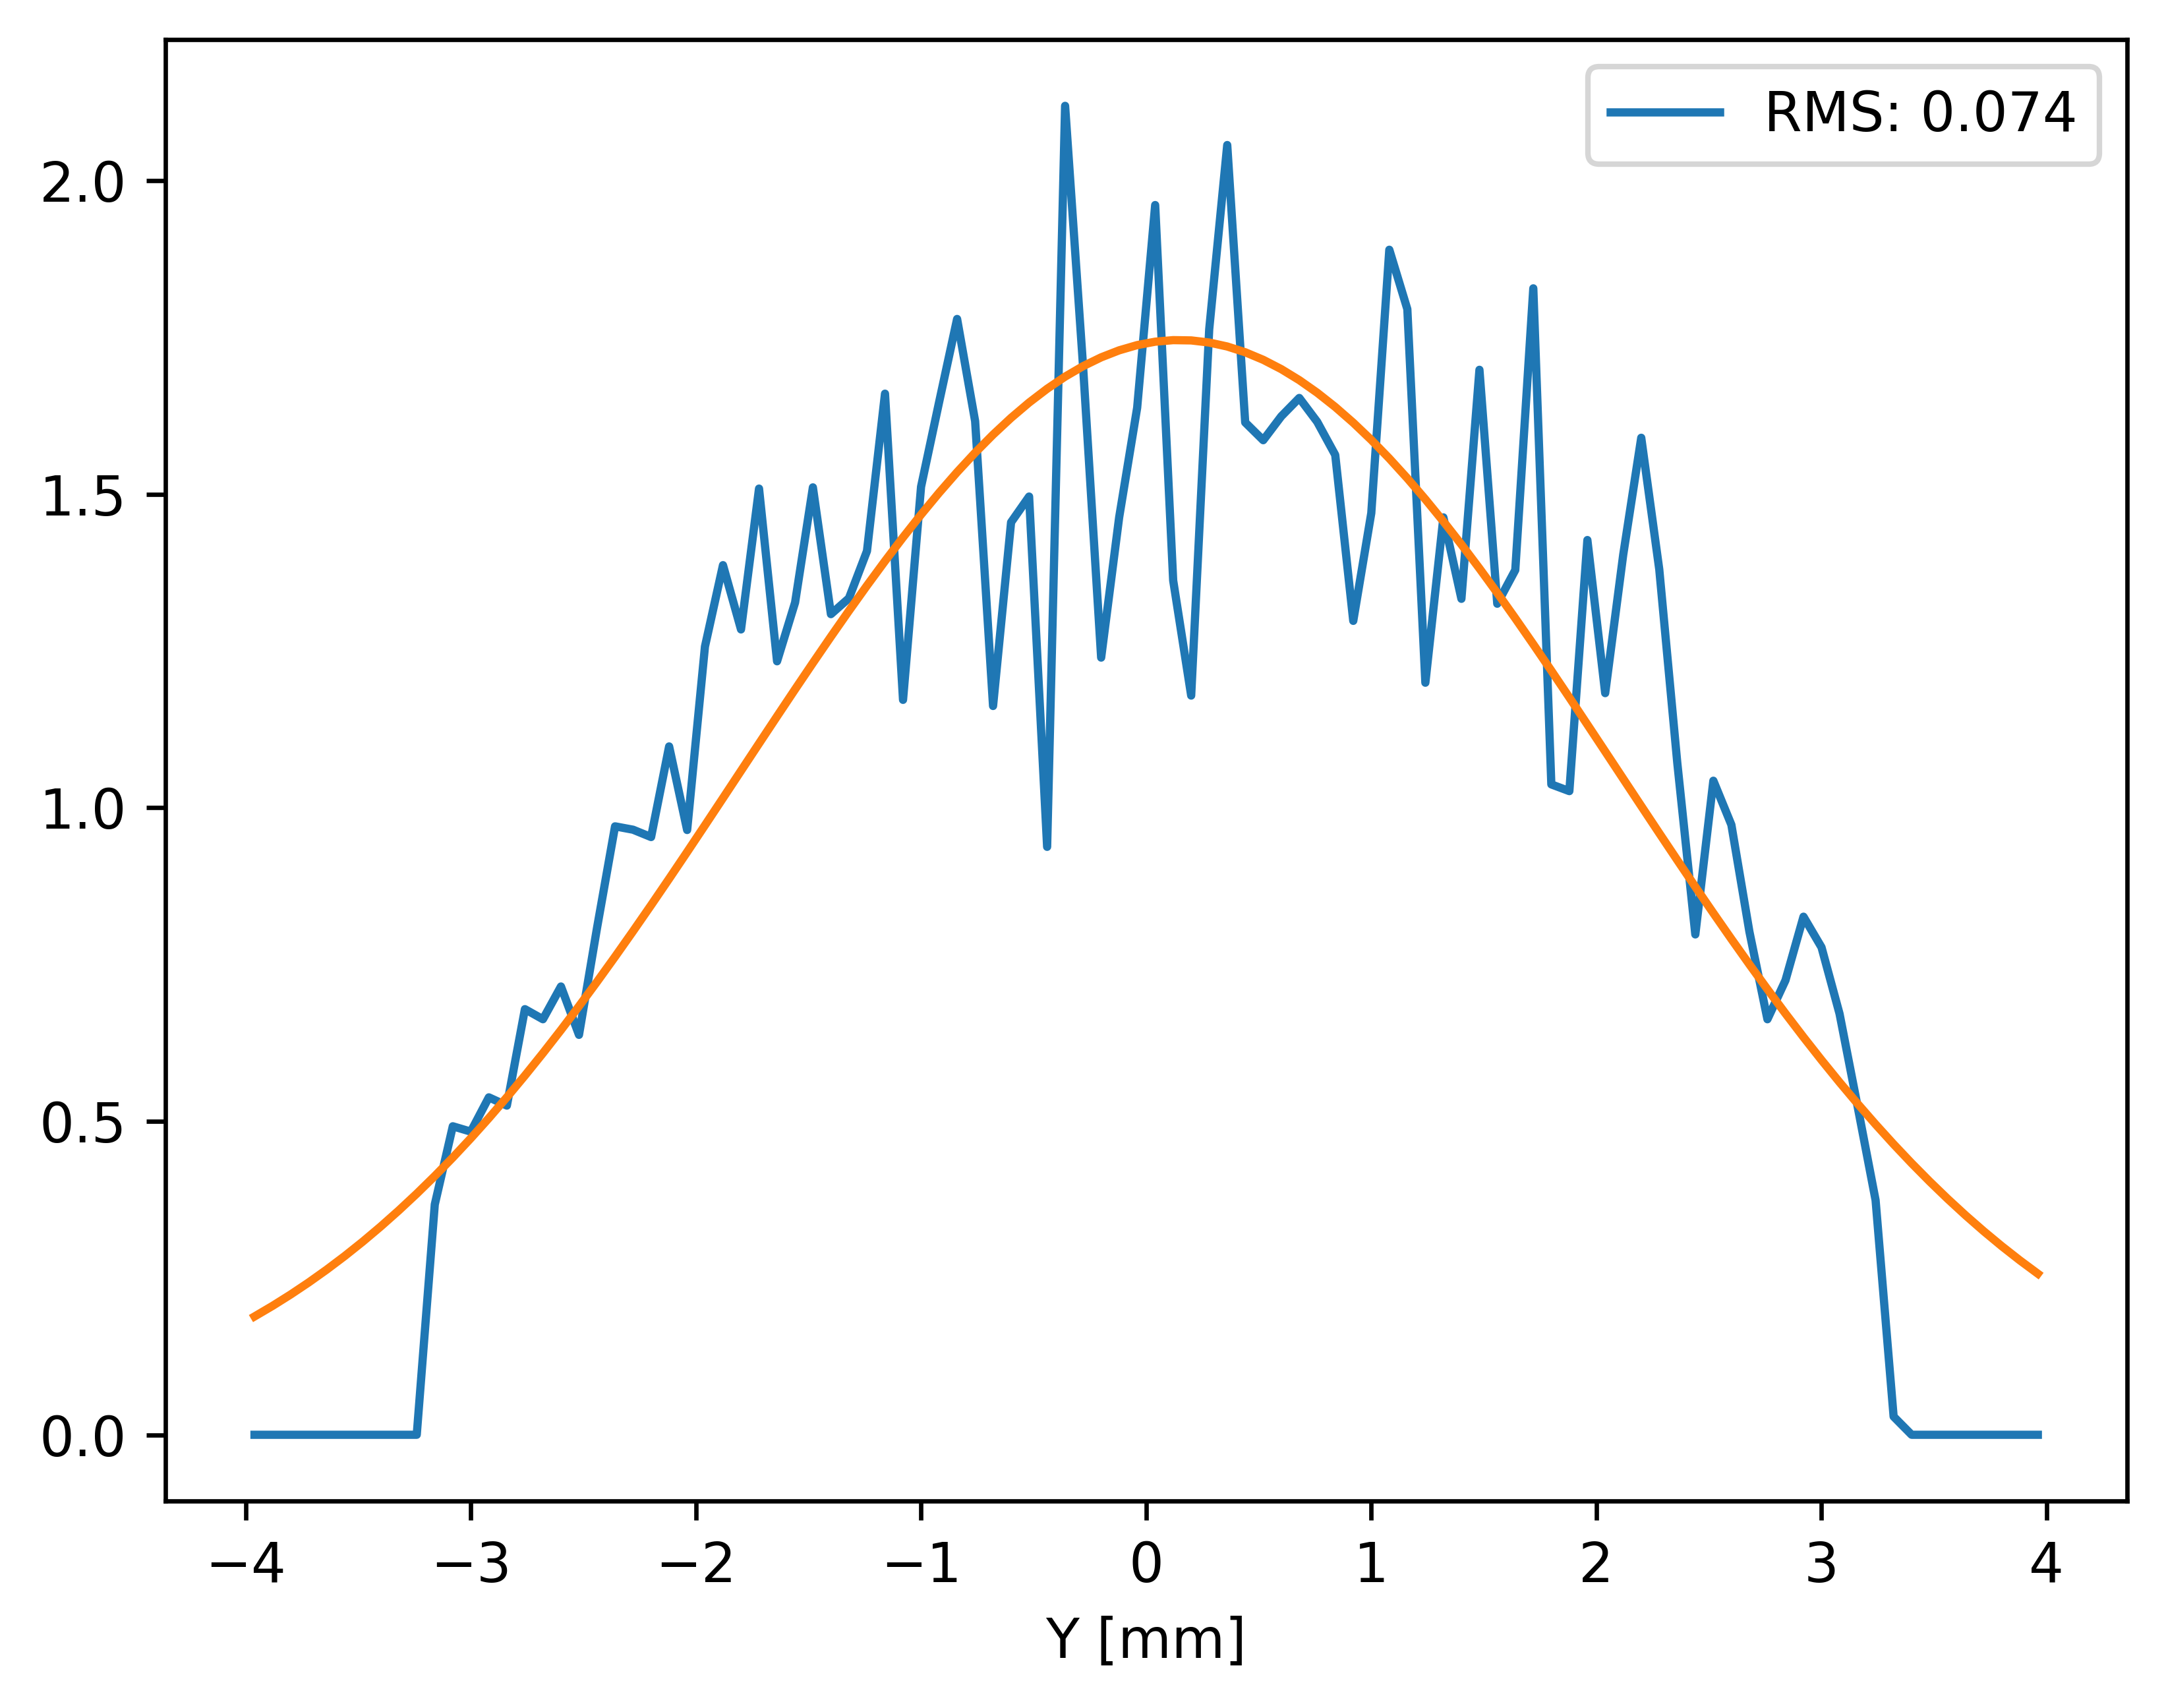
\includegraphics[width=0.9\linewidth]{./../figures/slope_error/WB4C_d30_d-spacing_gradient_45keV_slope_error025urad_Yprofile.png}
\caption{0.25 urad}
\label{fig:025urad}
\end{figure}

%%%%%%%%%%%%%%%%%%%%%%%%%%%%%%%%%%%%%%%%%%%%%%%%%%%%%%%%%%%%%%%%%%%%%%%%%%%%%%%%%%
\clearpage
\subsubsection{0.3 urad}
\begin{figure}[H]
\centering
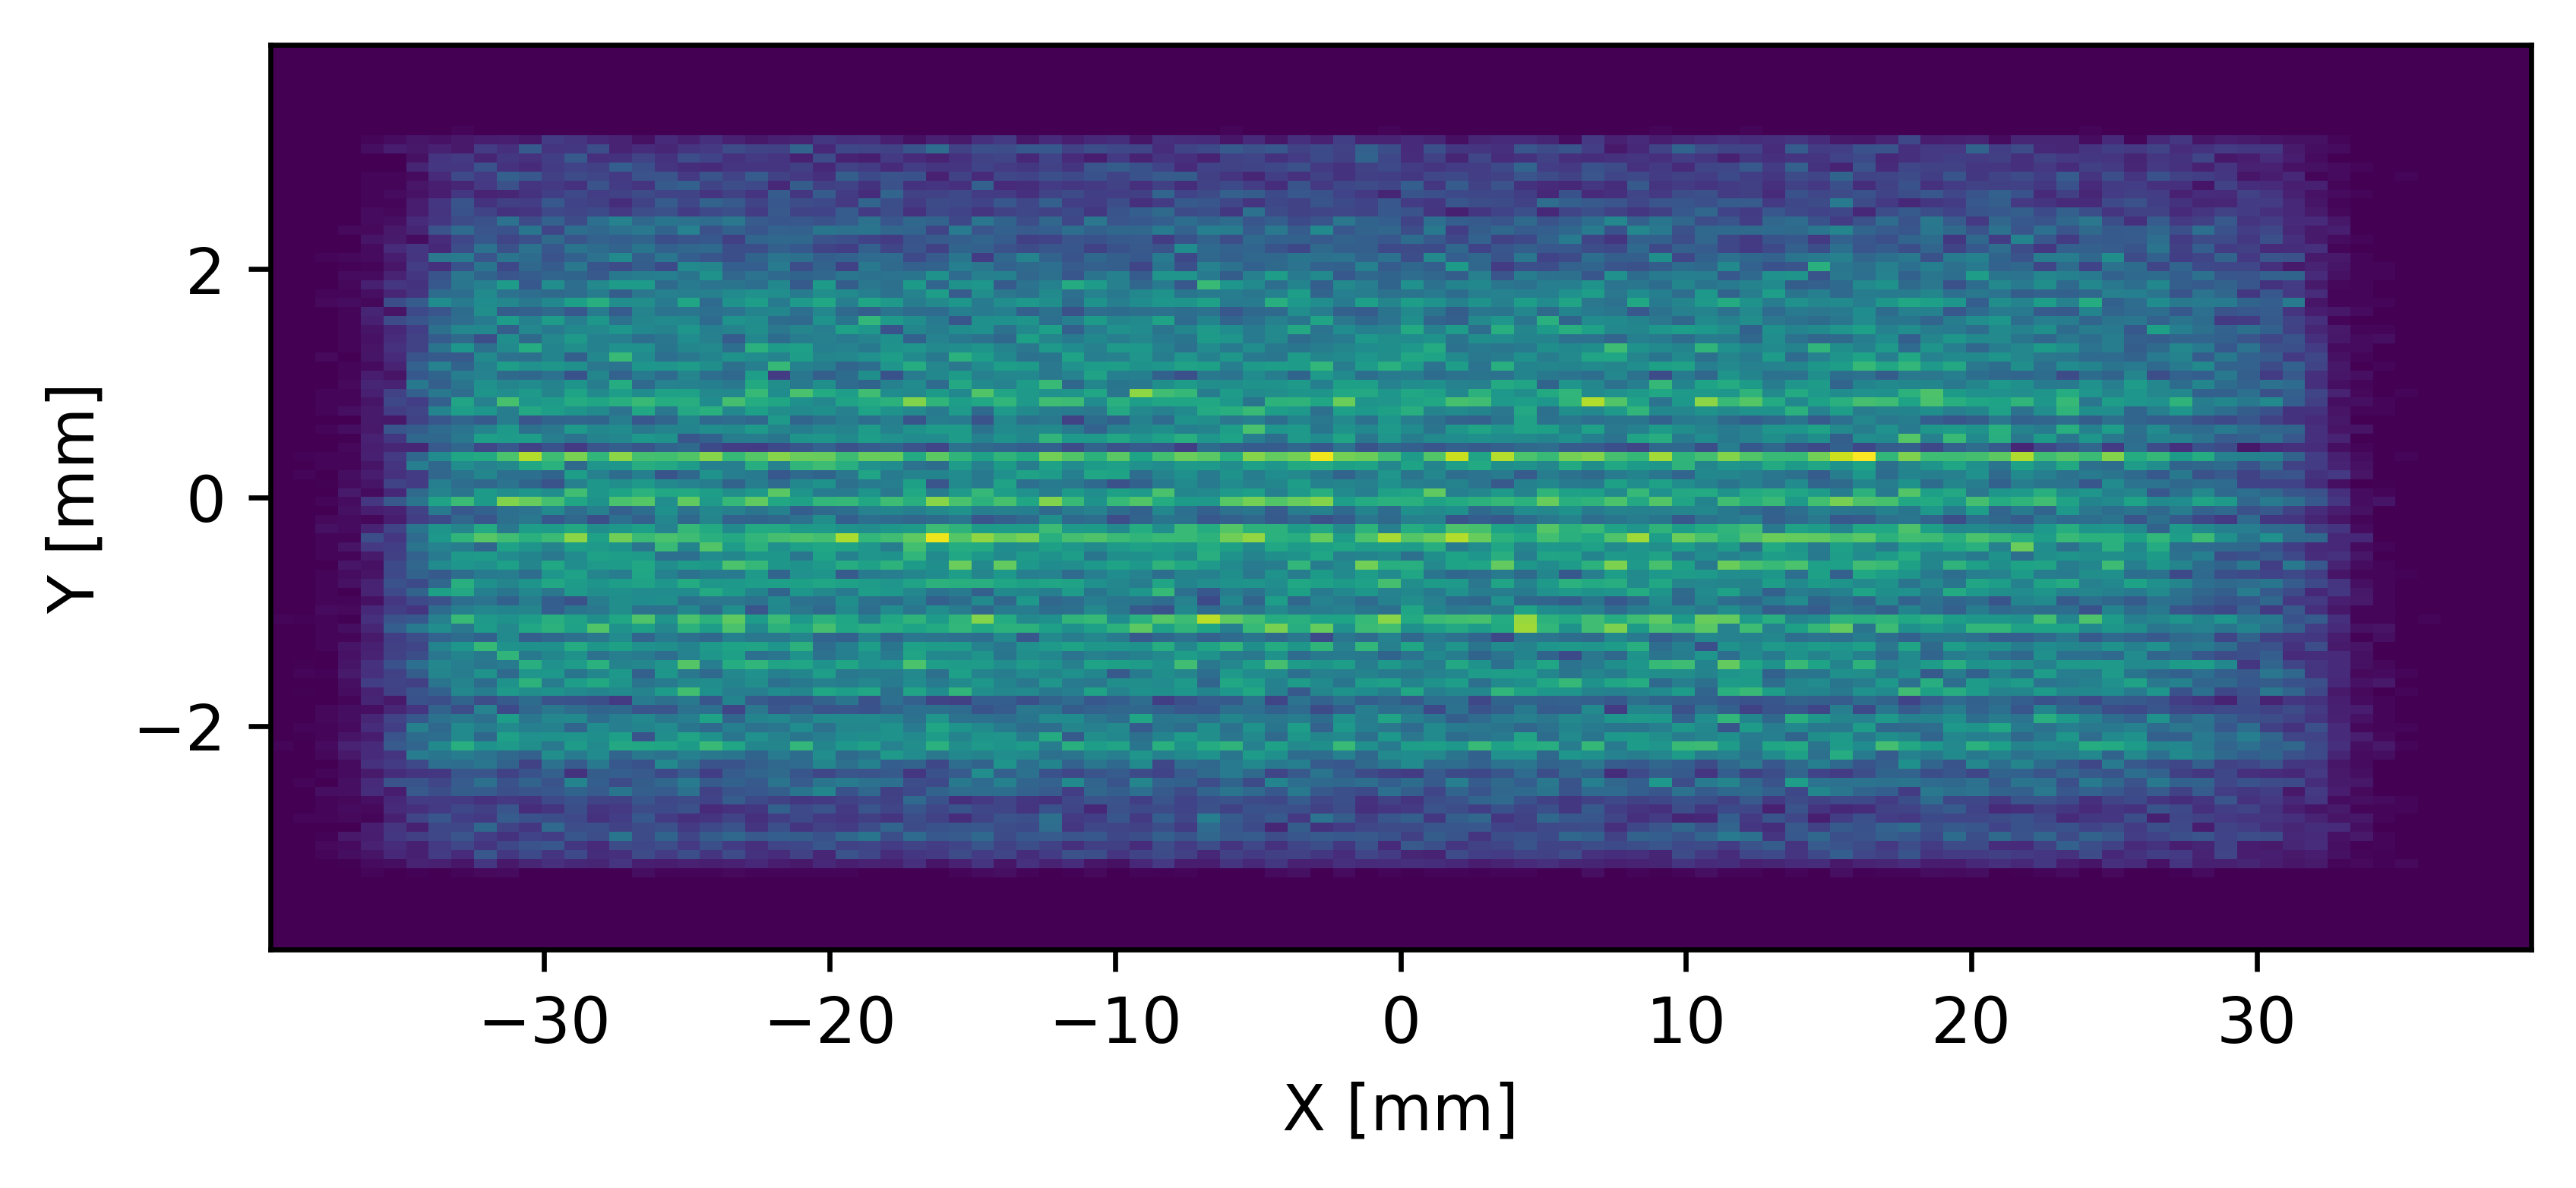
\includegraphics[width=0.9\linewidth]{./../figures/slope_error/WB4C_d30_d-spacing_gradient_45keV_slope_error03urad.png}
\end{figure}

\begin{figure}[H]
\centering
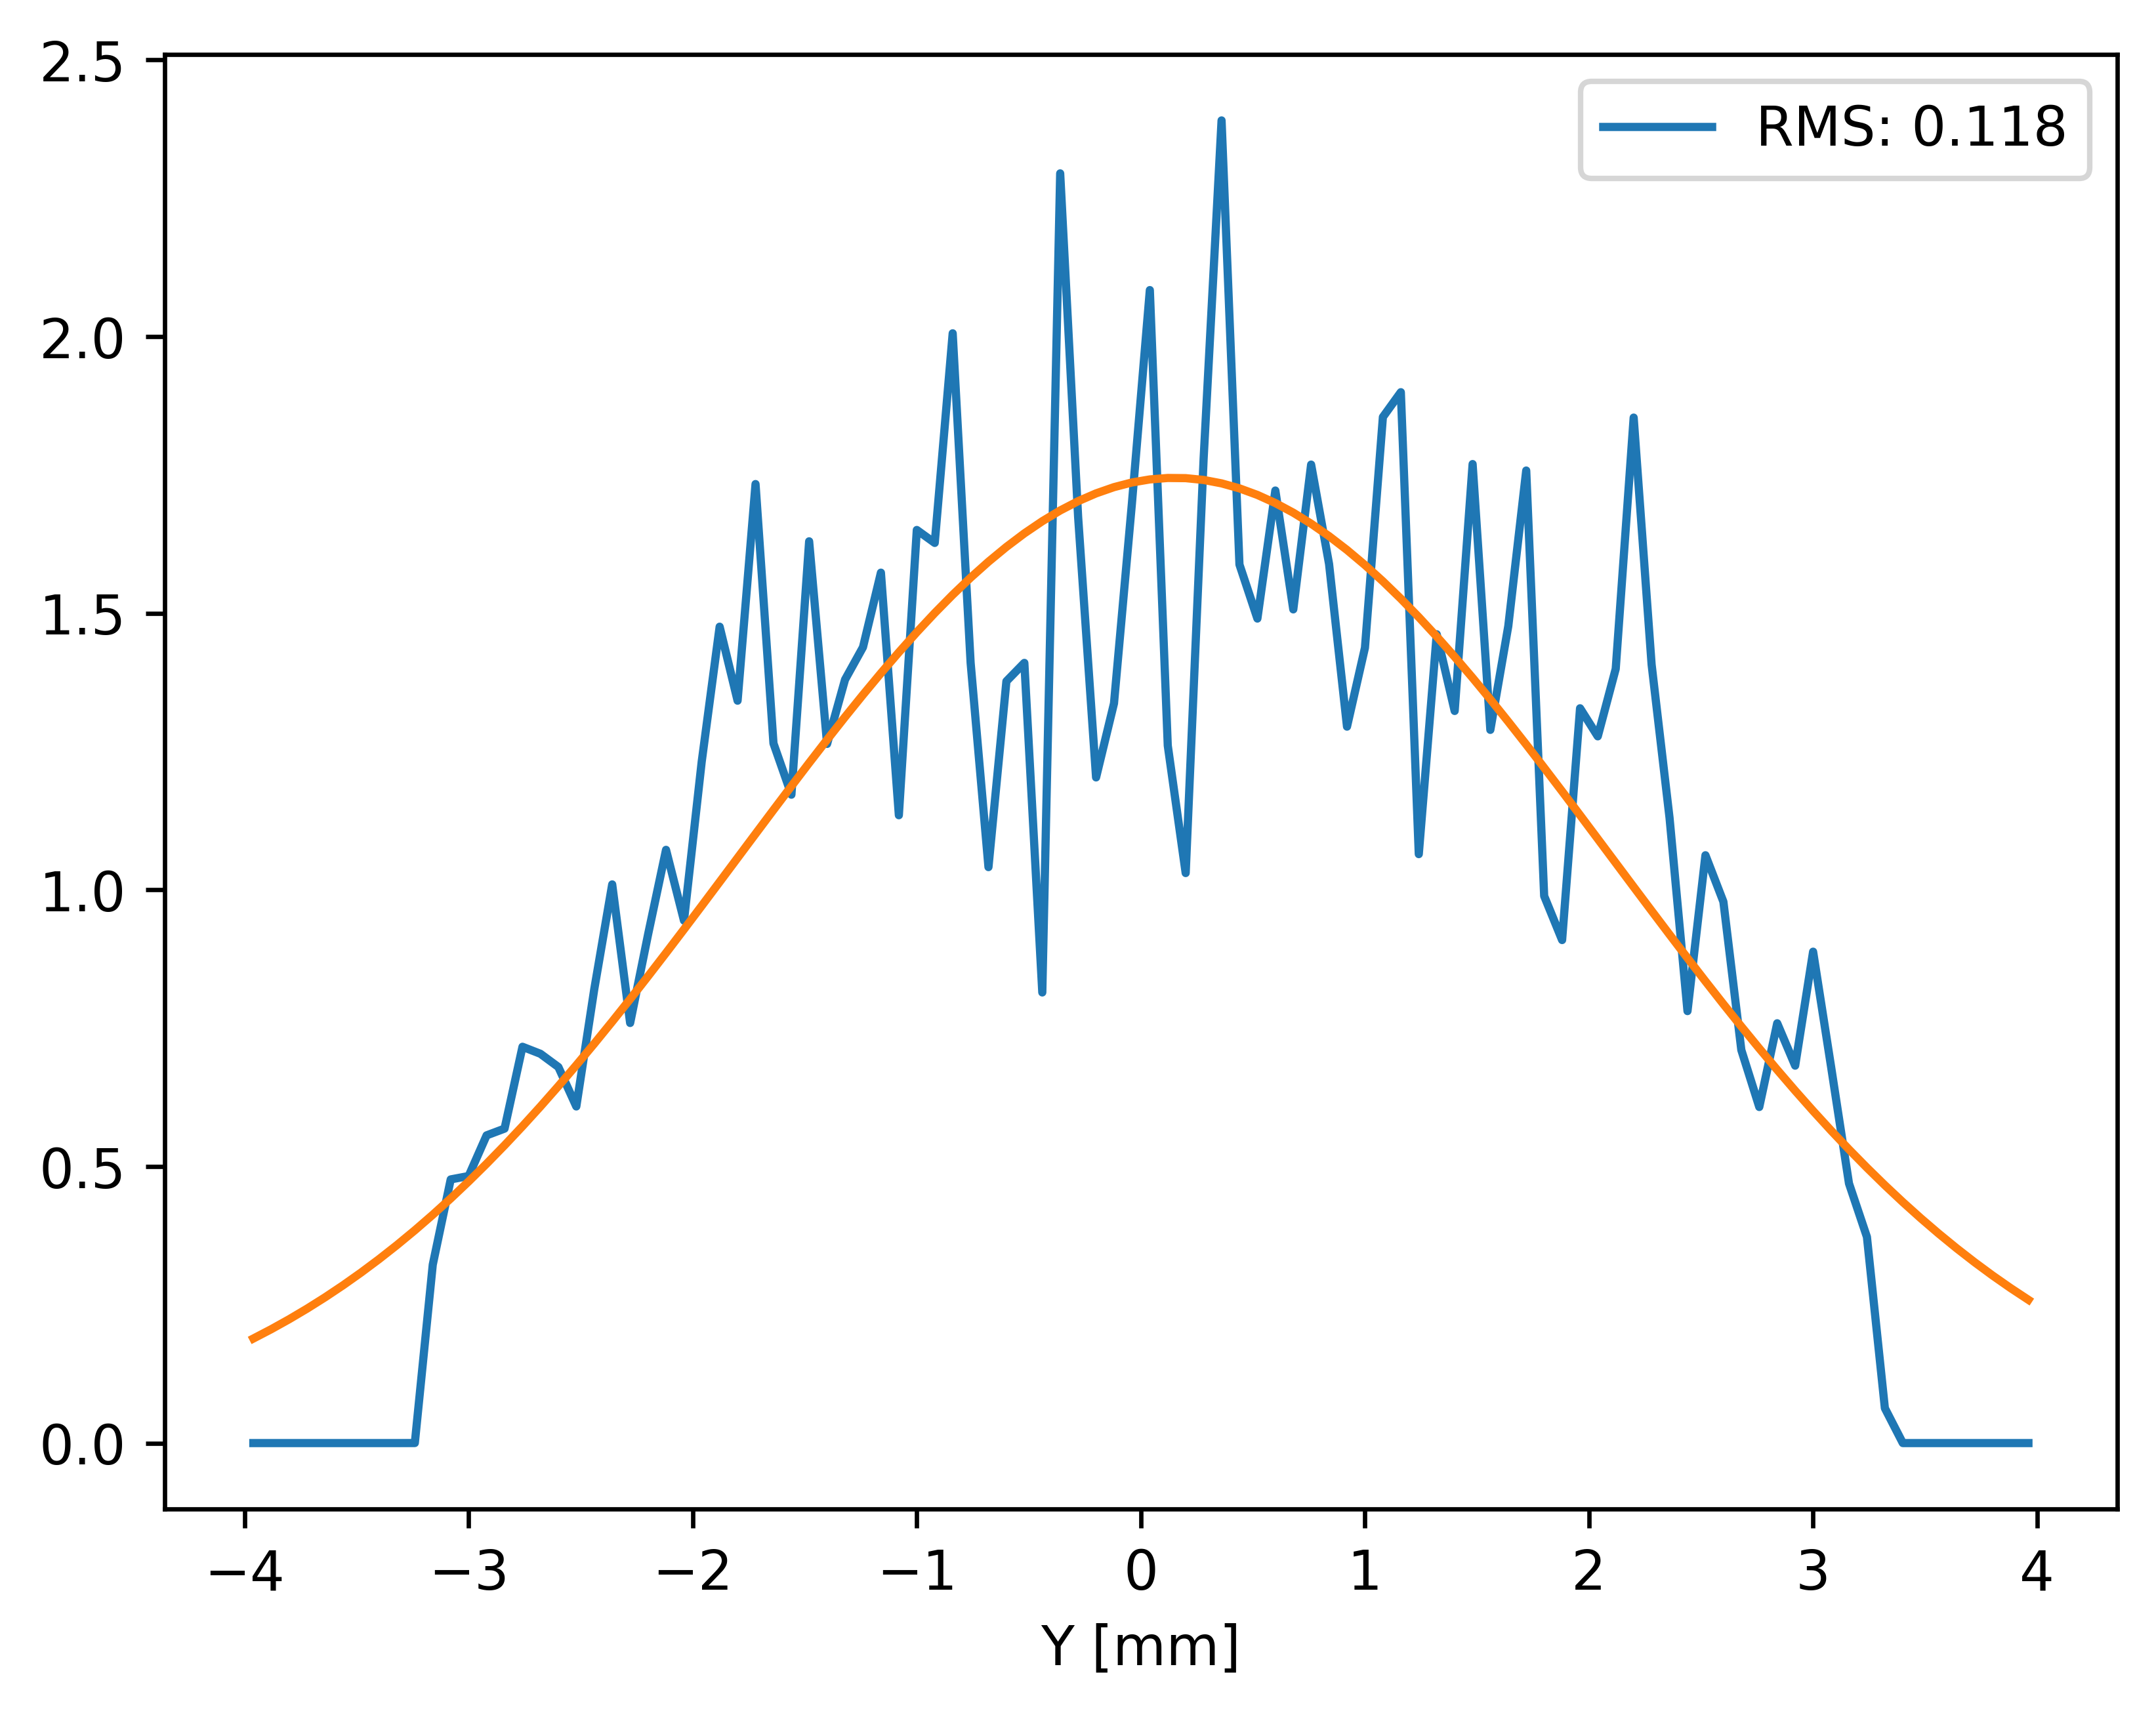
\includegraphics[width=0.9\linewidth]{./../figures/slope_error/WB4C_d30_d-spacing_gradient_45keV_slope_error03urad_Yprofile.png}
\caption{0.3 urad}
\label{fig:03urad}
\end{figure}

%%%%%%%%%%%%%%%%%%%%%%%%%%%%%%%%%%%%%%%%%%%%%%%%%%%%%%%%%%%%%%%%%%%%%%%%%%%%%%%%%%
\clearpage
\subsubsection{0.35 urad}
\begin{figure}[H]
\centering
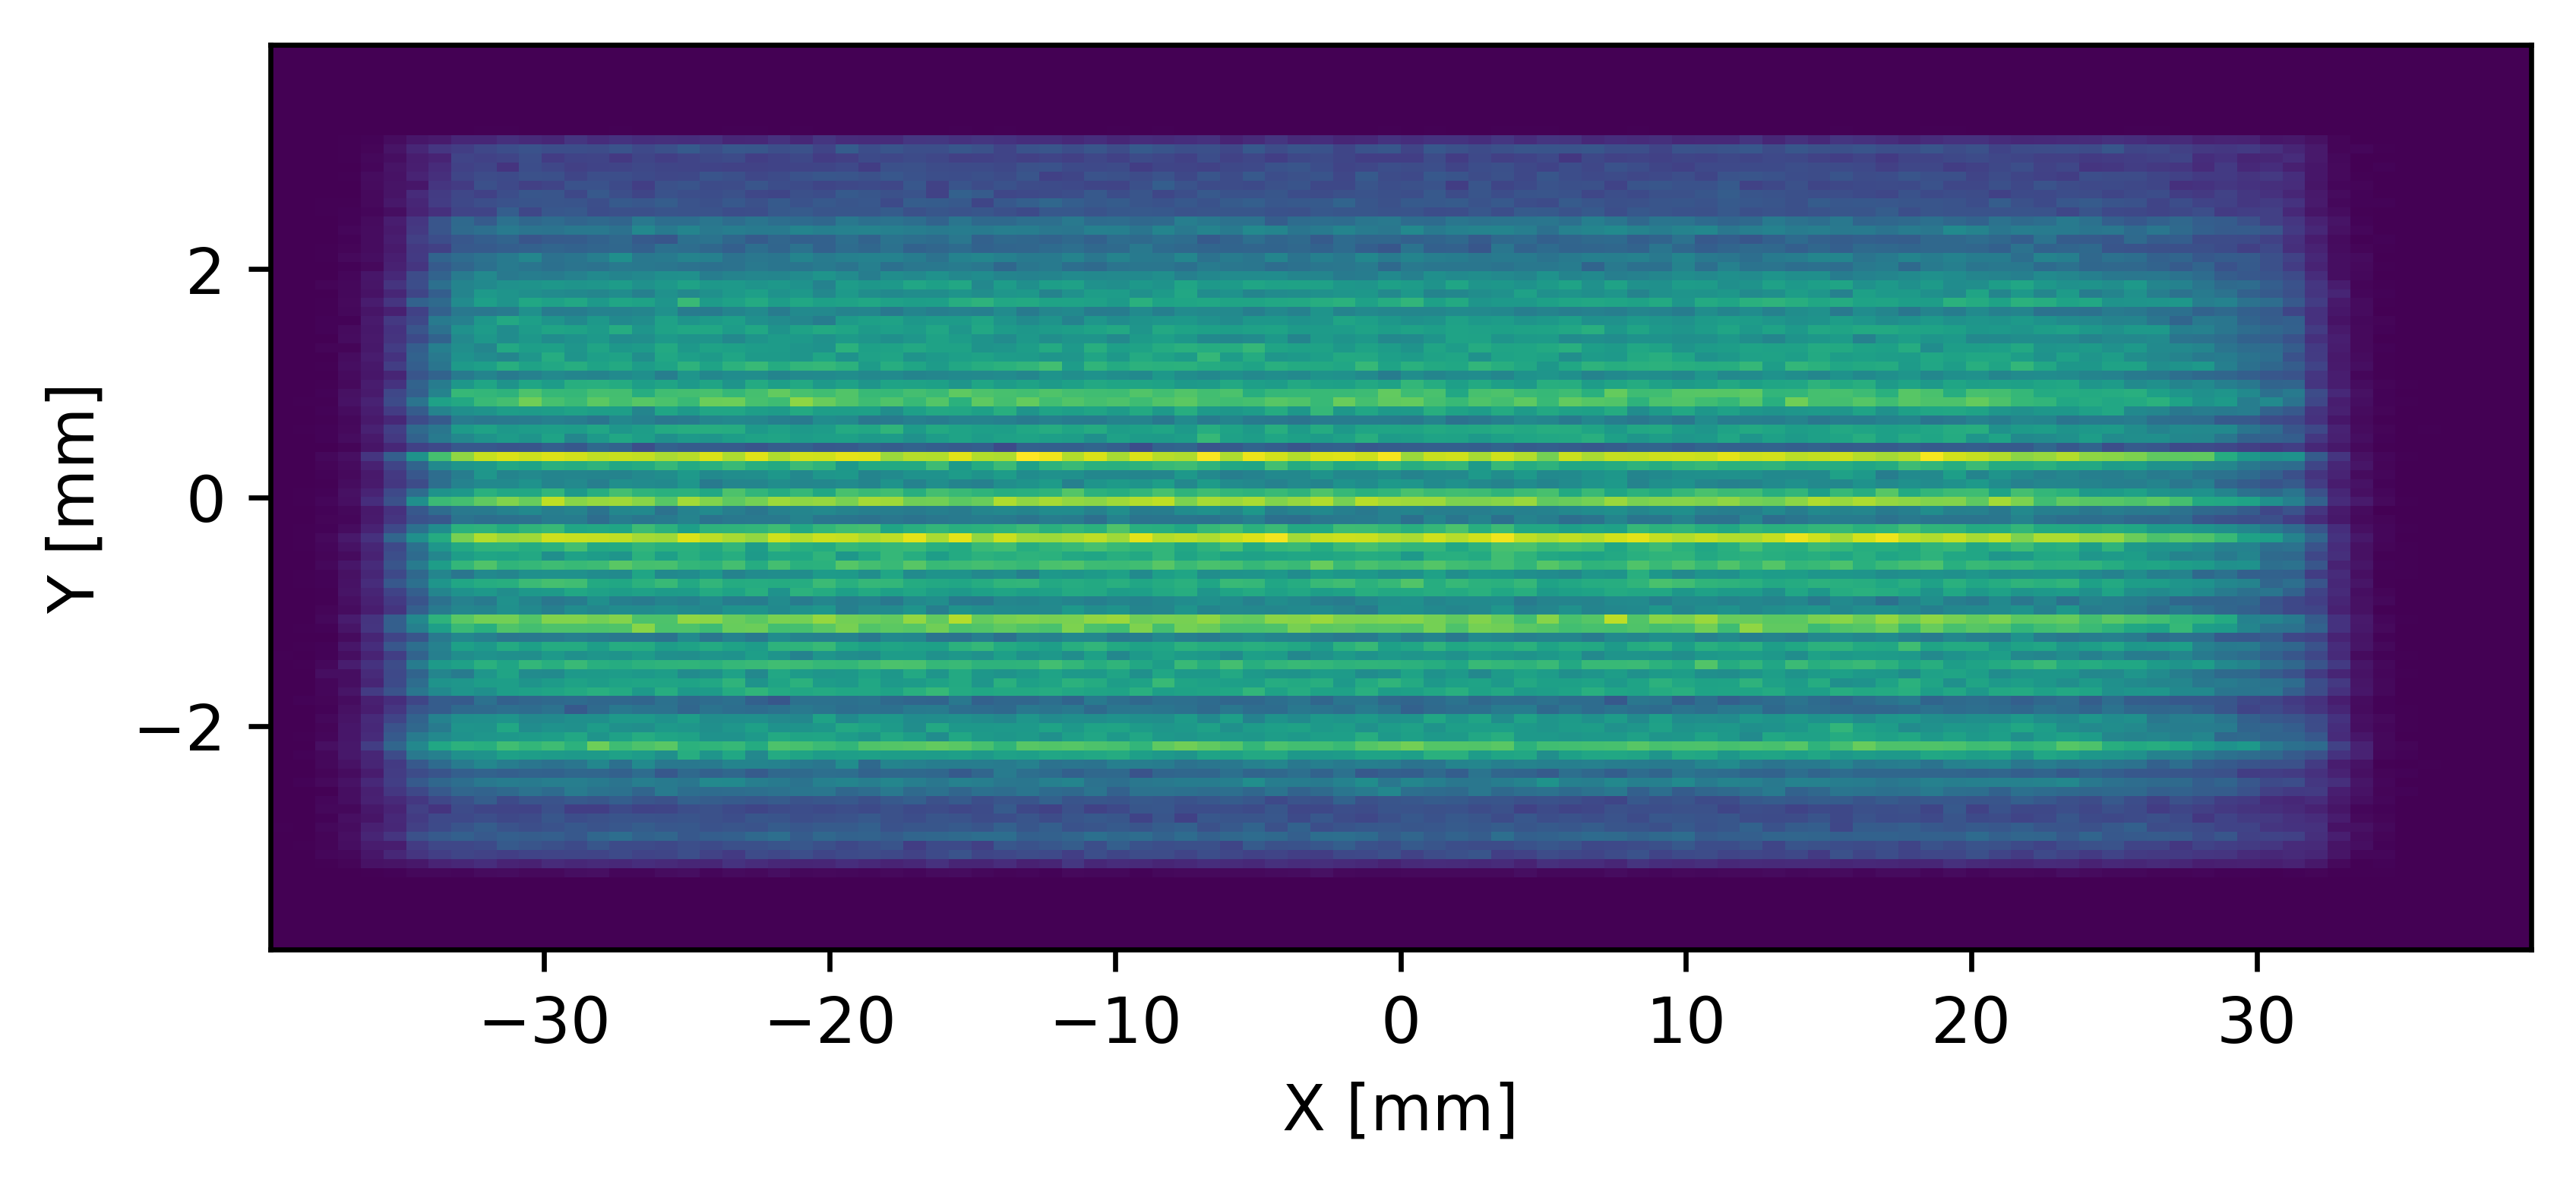
\includegraphics[width=0.9\linewidth]{./../figures/slope_error/WB4C_d30_d-spacing_gradient_45keV_slope_error035urad.png}
\end{figure}

\begin{figure}[H]
\centering
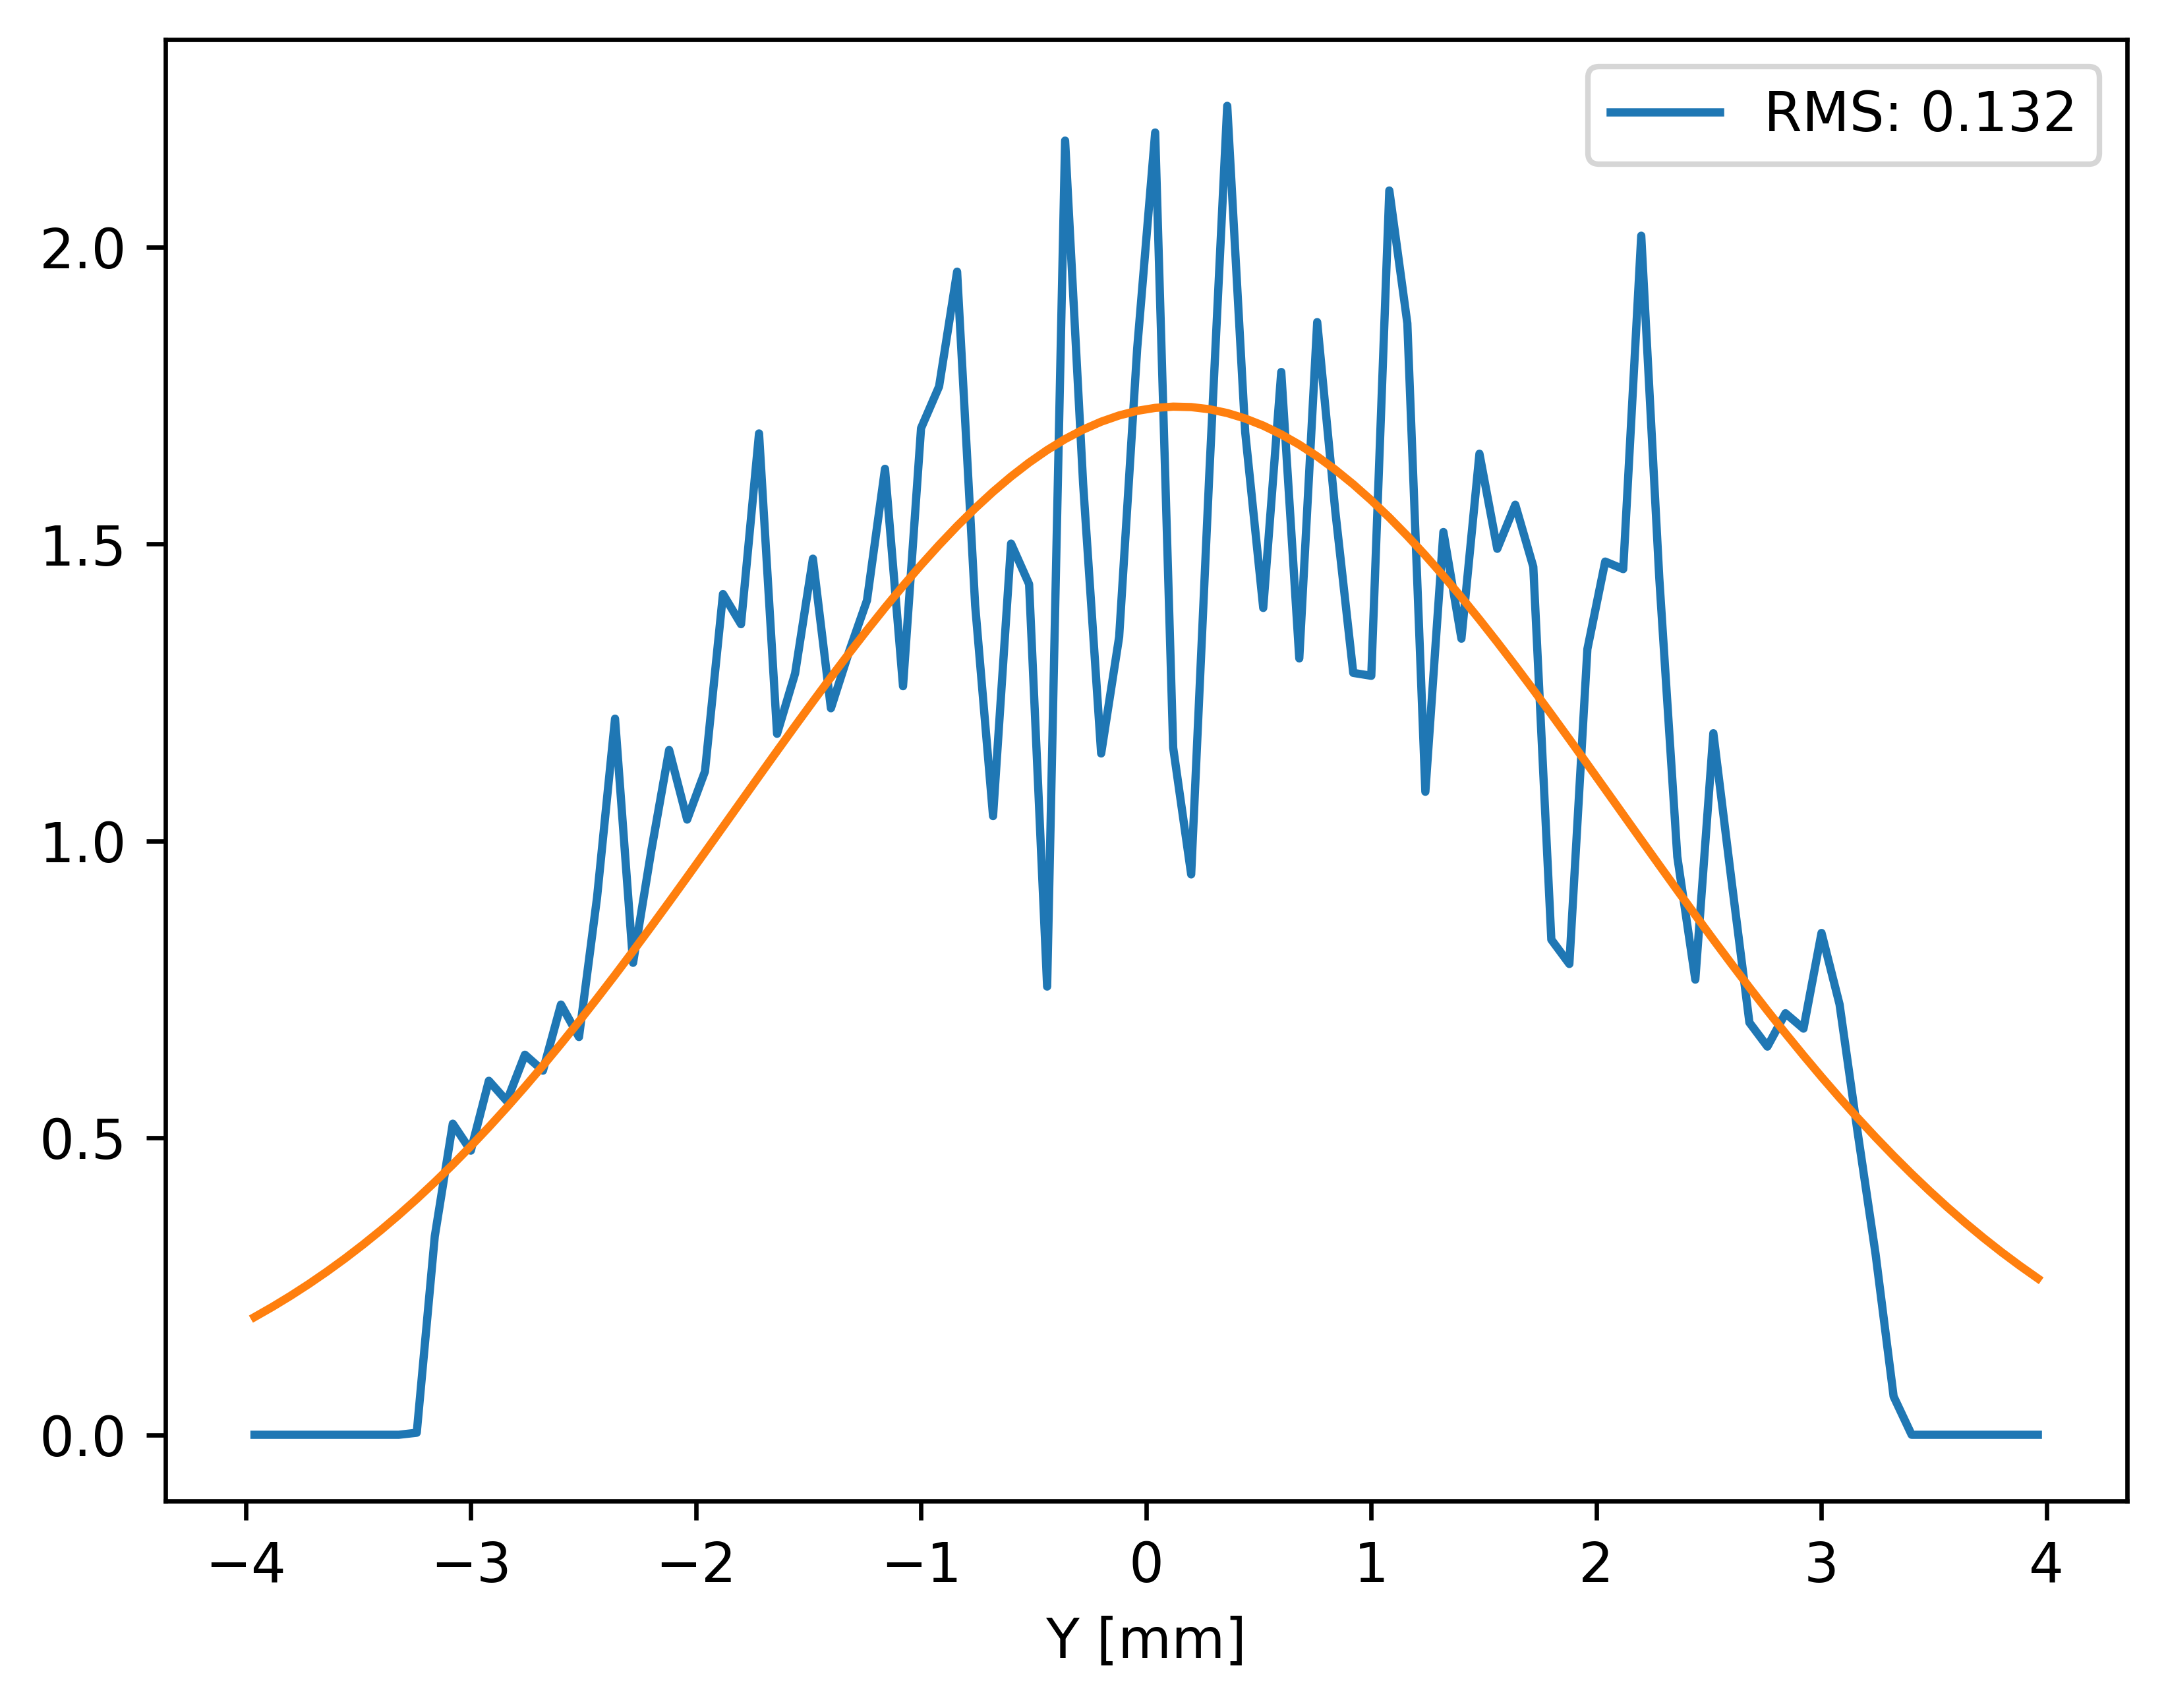
\includegraphics[width=0.9\linewidth]{./../figures/slope_error/WB4C_d30_d-spacing_gradient_45keV_slope_error035urad_Yprofile.png}
\caption{0.35 urad}
\label{fig:035urad}
\end{figure}

%%%%%%%%%%%%%%%%%%%%%%%%%%%%%%%%%%%%%%%%%%%%%%%%%%%%%%%%%%%%%%%%%%%%%%%%%%%%%%%%%%
\clearpage
\subsubsection{0.4 urad}
\begin{figure}[H]
\centering
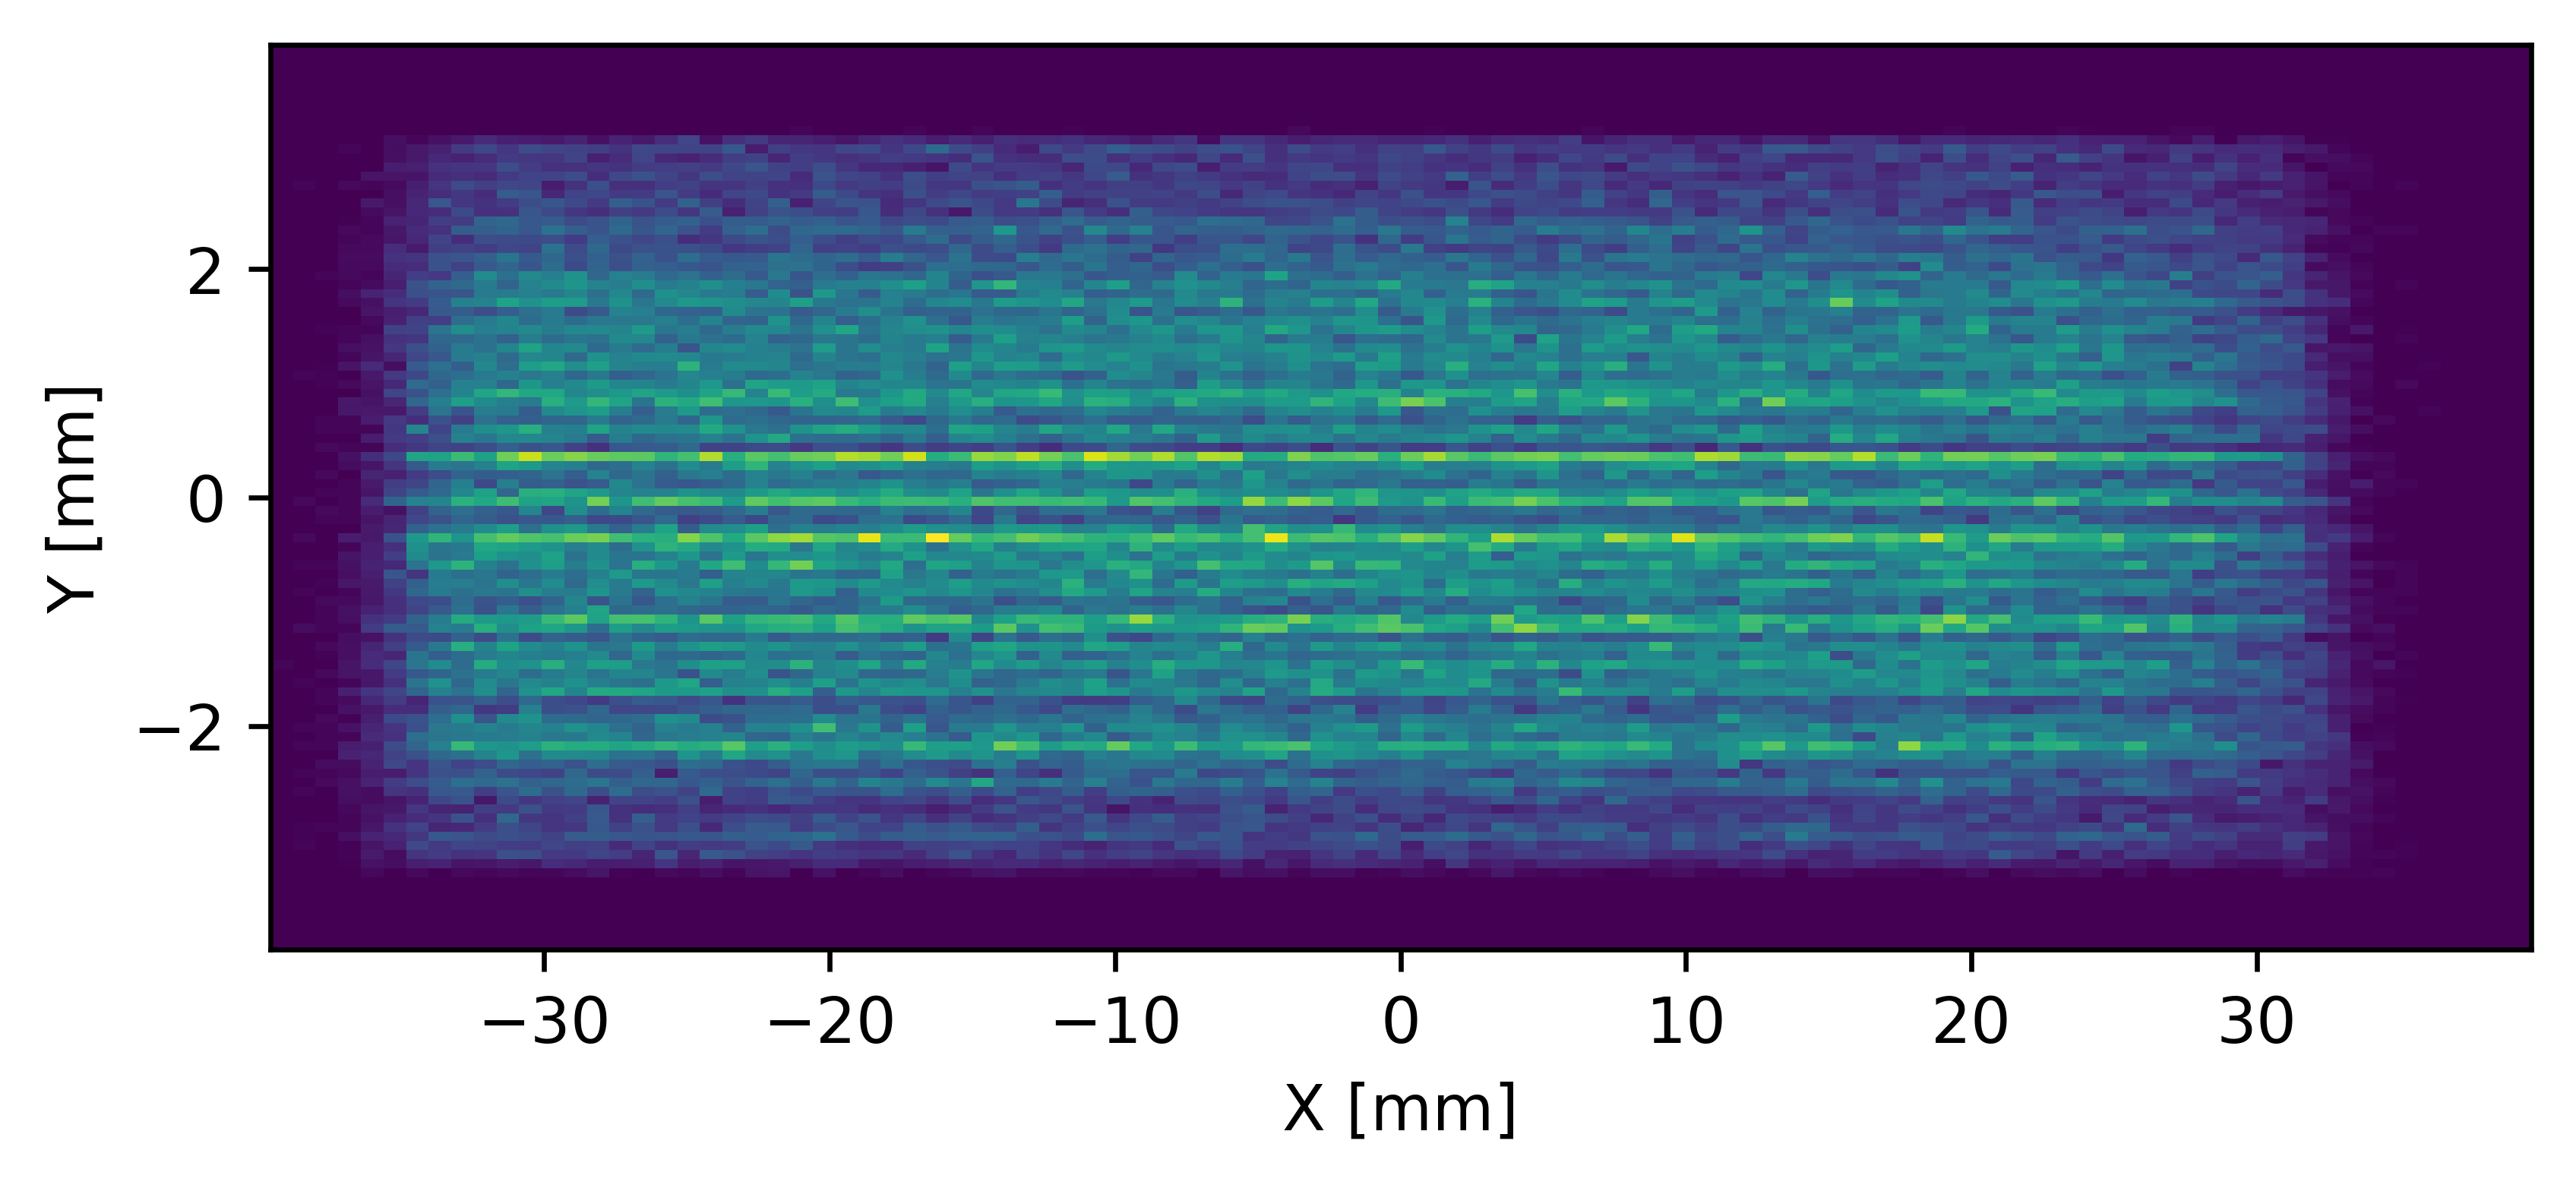
\includegraphics[width=0.9\linewidth]{./../figures/slope_error/WB4C_d30_d-spacing_gradient_45keV_slope_error04urad.png}
\end{figure}

\begin{figure}[H]
\centering
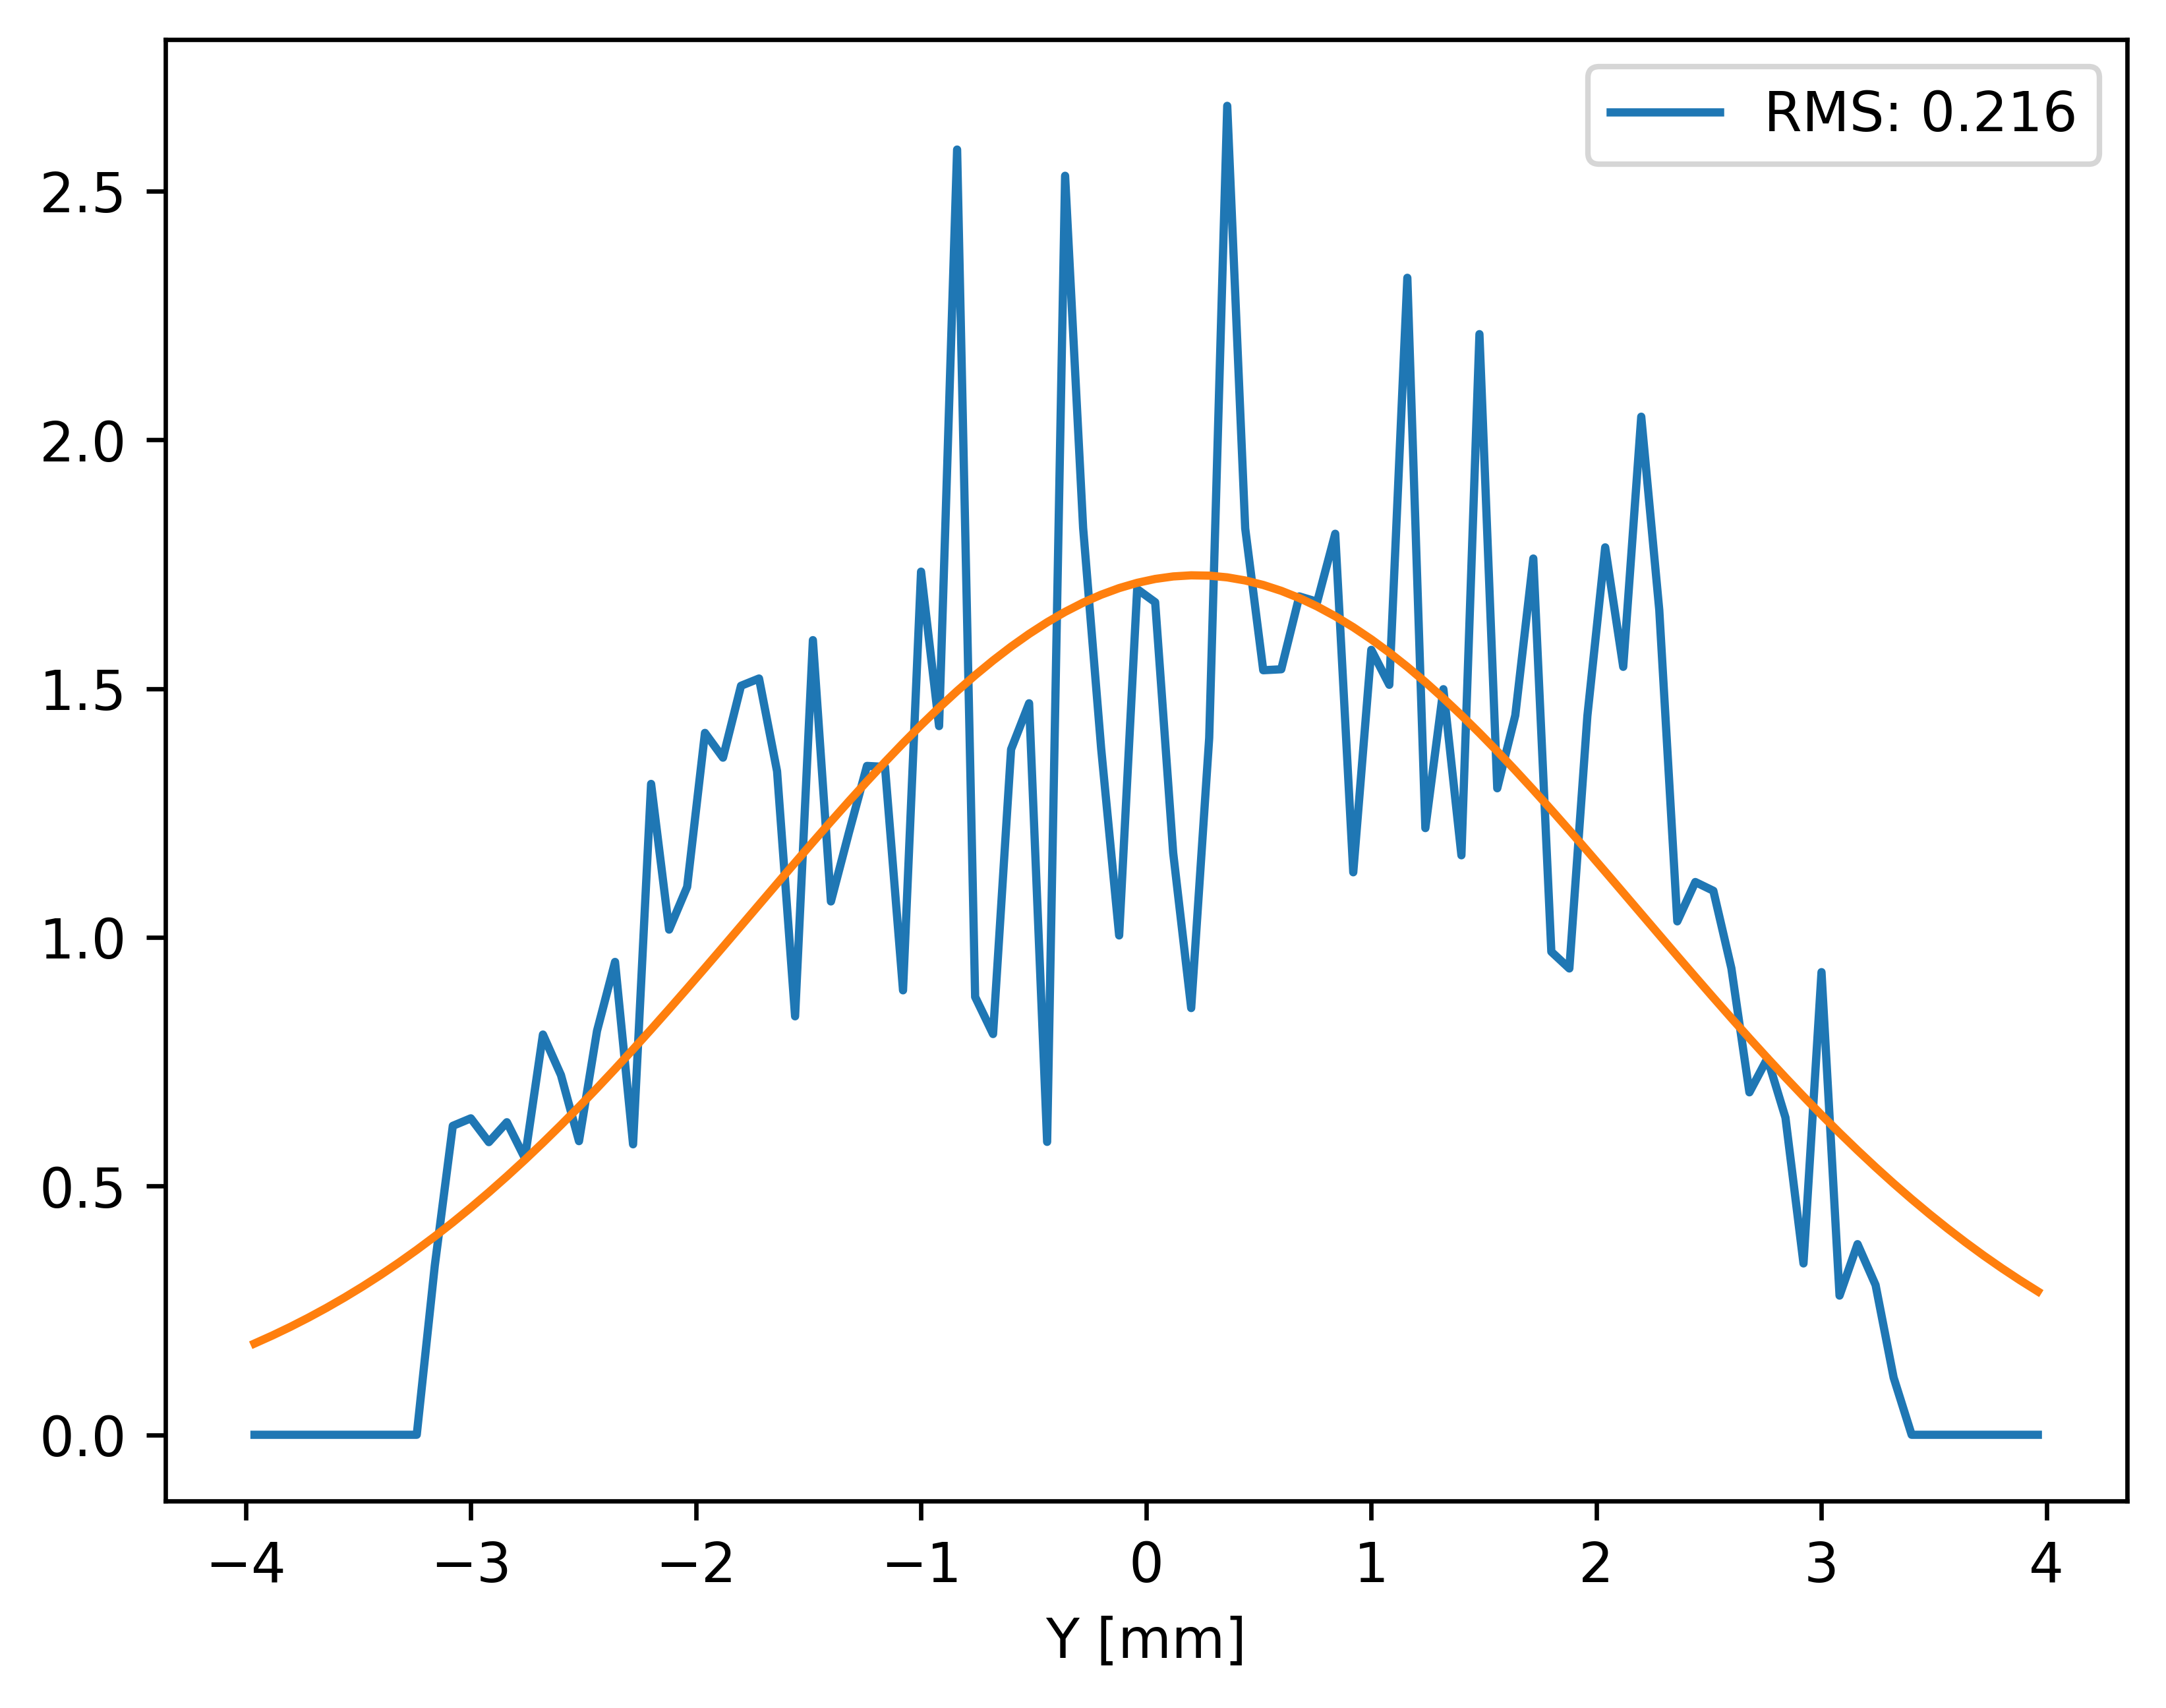
\includegraphics[width=0.9\linewidth]{./../figures/slope_error/WB4C_d30_d-spacing_gradient_45keV_slope_error04urad_Yprofile.png}
\caption{0.4 urad}
\label{fig:04urad}
\end{figure}

%%%%%%%%%%%%%%%%%%%%%%%%%%%%%%%%%%%%%%%%%%%%%%%%%%%%%%%%%%%%%%%%%%%%%%%%%%%%%%%%%%
\clearpage
\subsubsection{0.5 urad}
\begin{figure}[H]
\centering
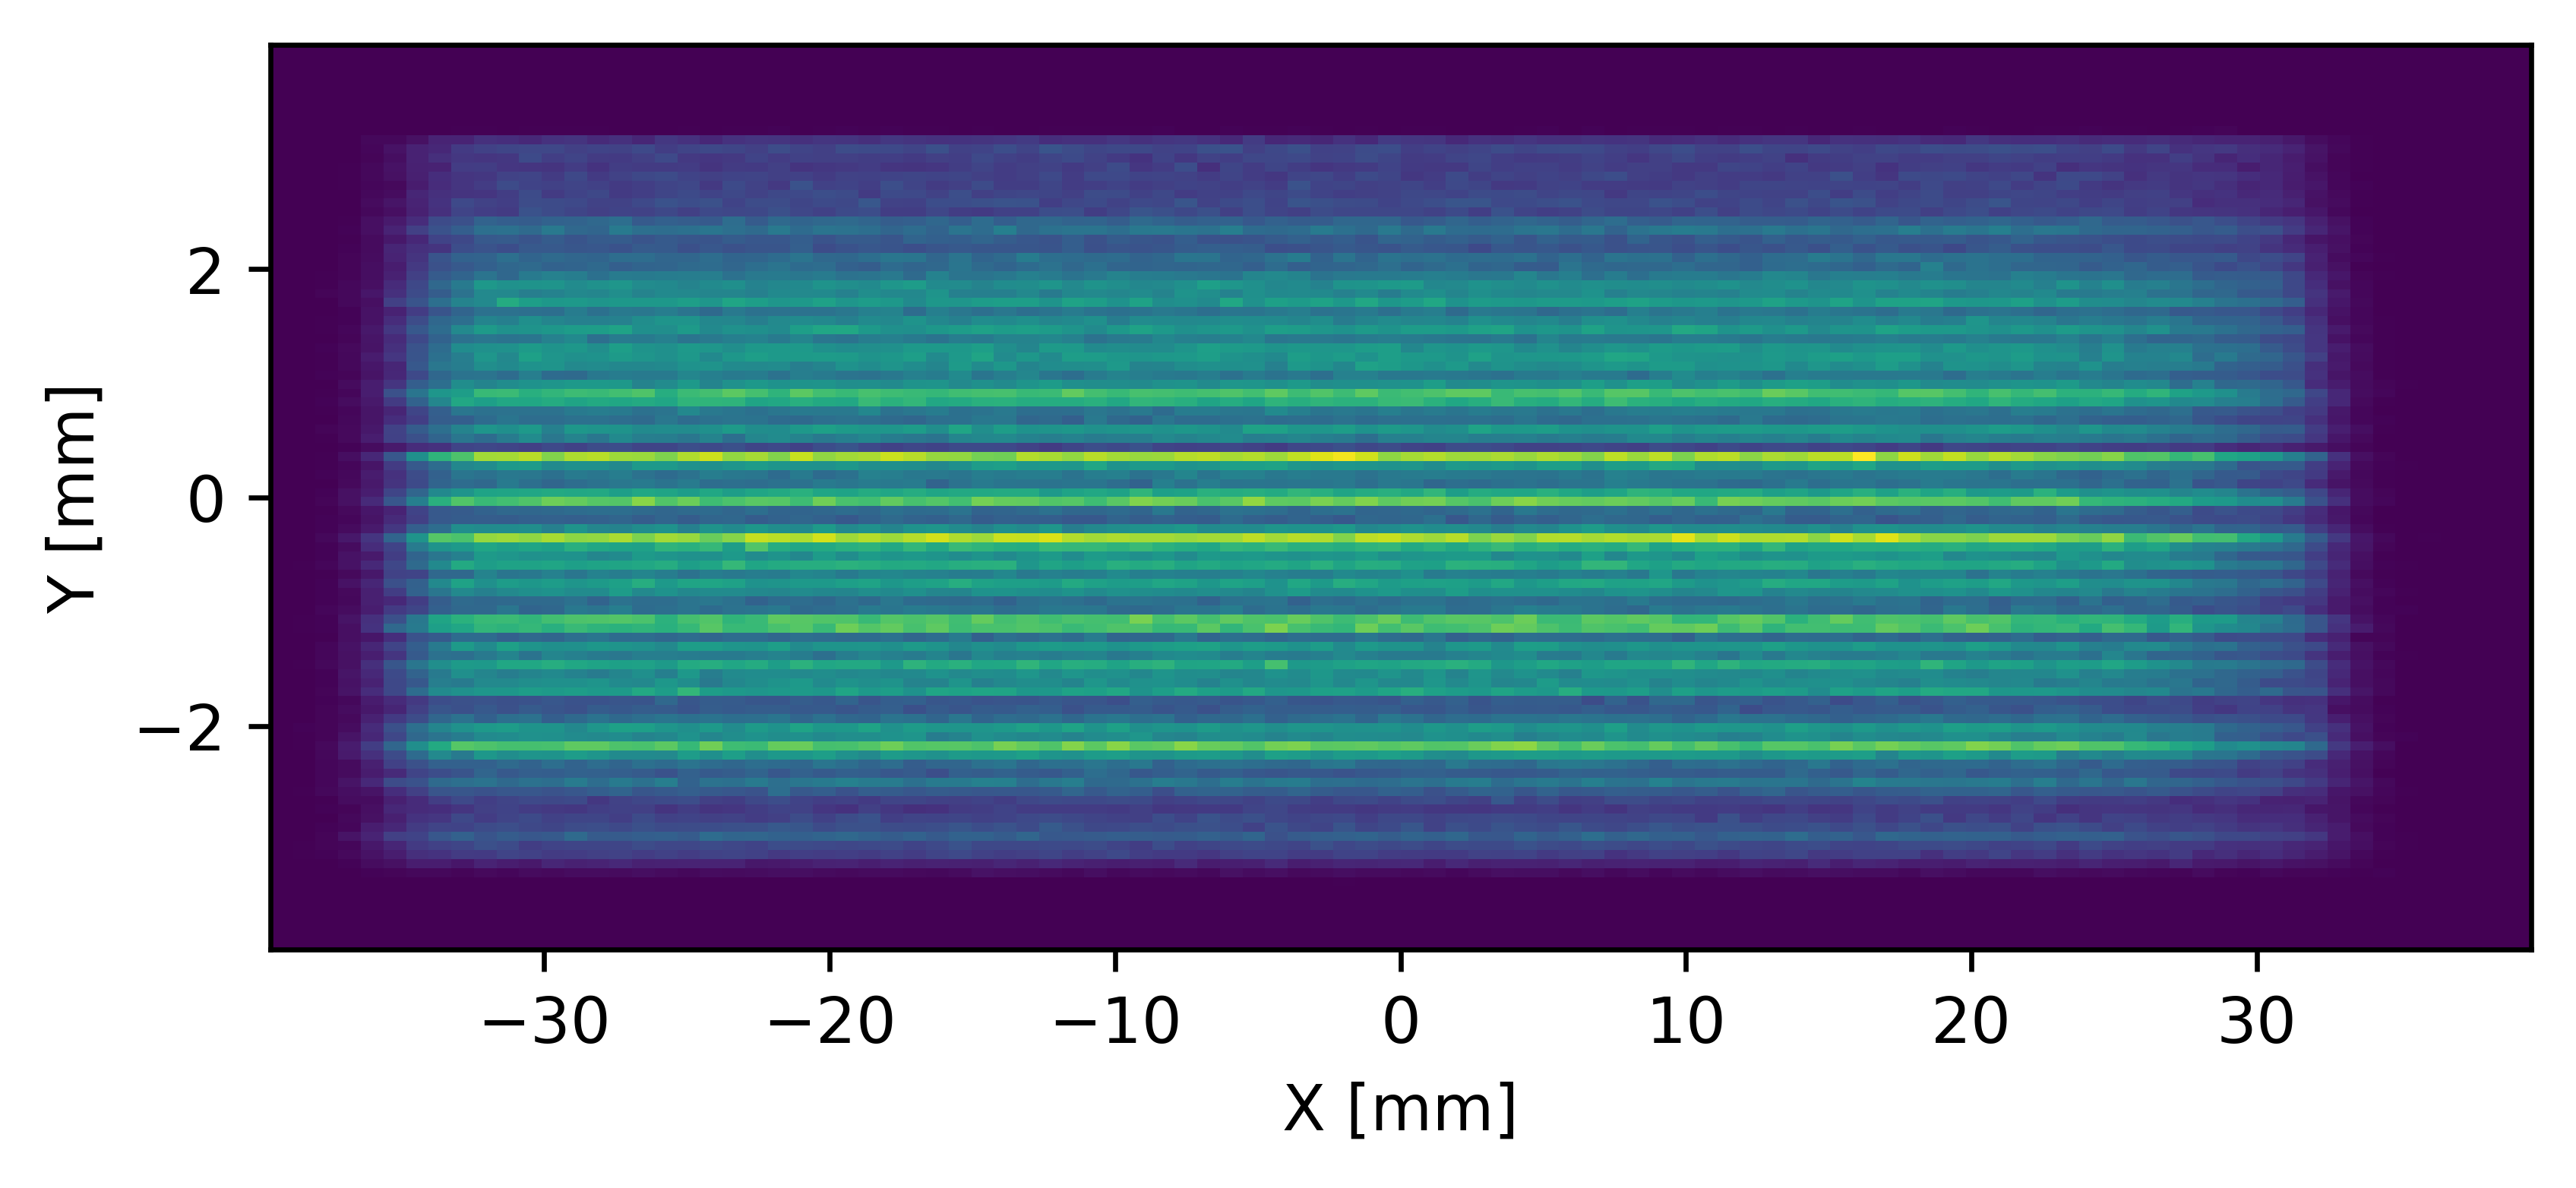
\includegraphics[width=0.9\linewidth]{./../figures/slope_error/WB4C_d30_d-spacing_gradient_45keV_slope_error05urad.png}
\end{figure}

\begin{figure}[H]
\centering
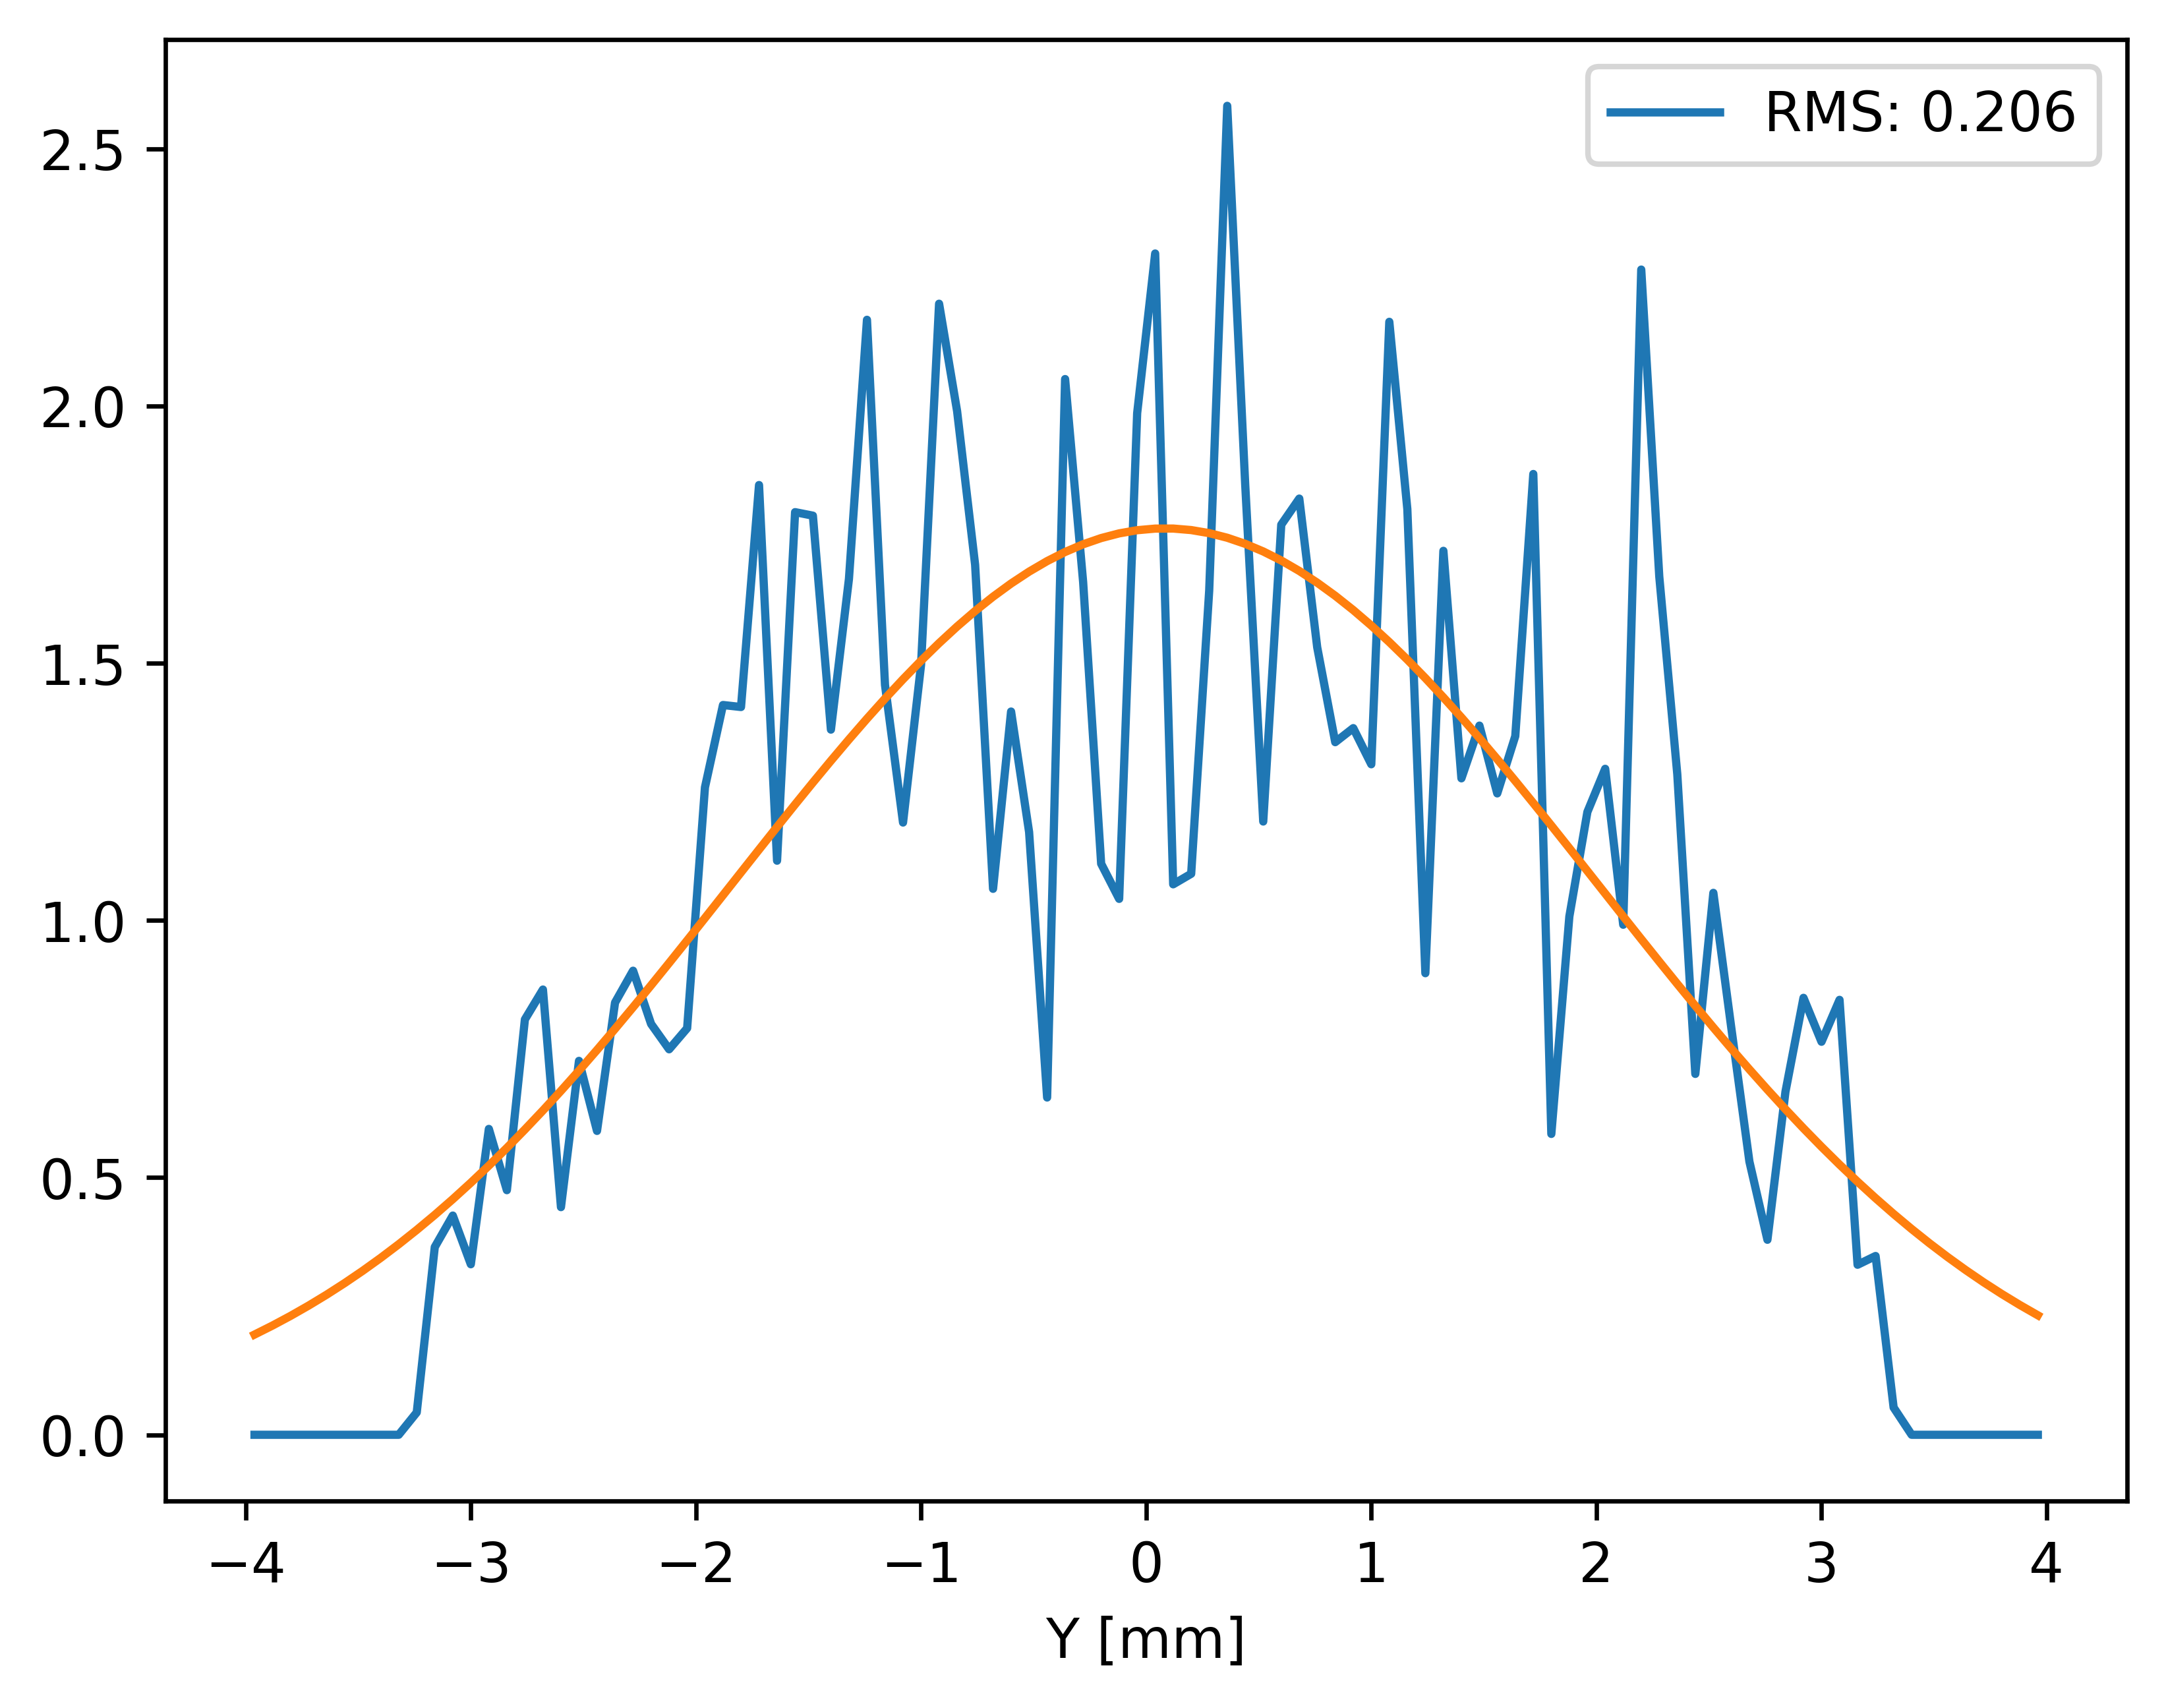
\includegraphics[width=0.9\linewidth]{./../figures/slope_error/WB4C_d30_d-spacing_gradient_45keV_slope_error05urad_Yprofile.png}
\caption{0.5 urad}
\label{fig:05urad}
\end{figure}

\clearpage
\subsection{Mirror slope error - ESRF ID19 source}
The ESRF ID19 PW150 source is considered for this paragraph for comparison. All remaining BL and mirror components are identical. 

\subsubsection{0.1 urad}
\begin{figure}[H]
\centering
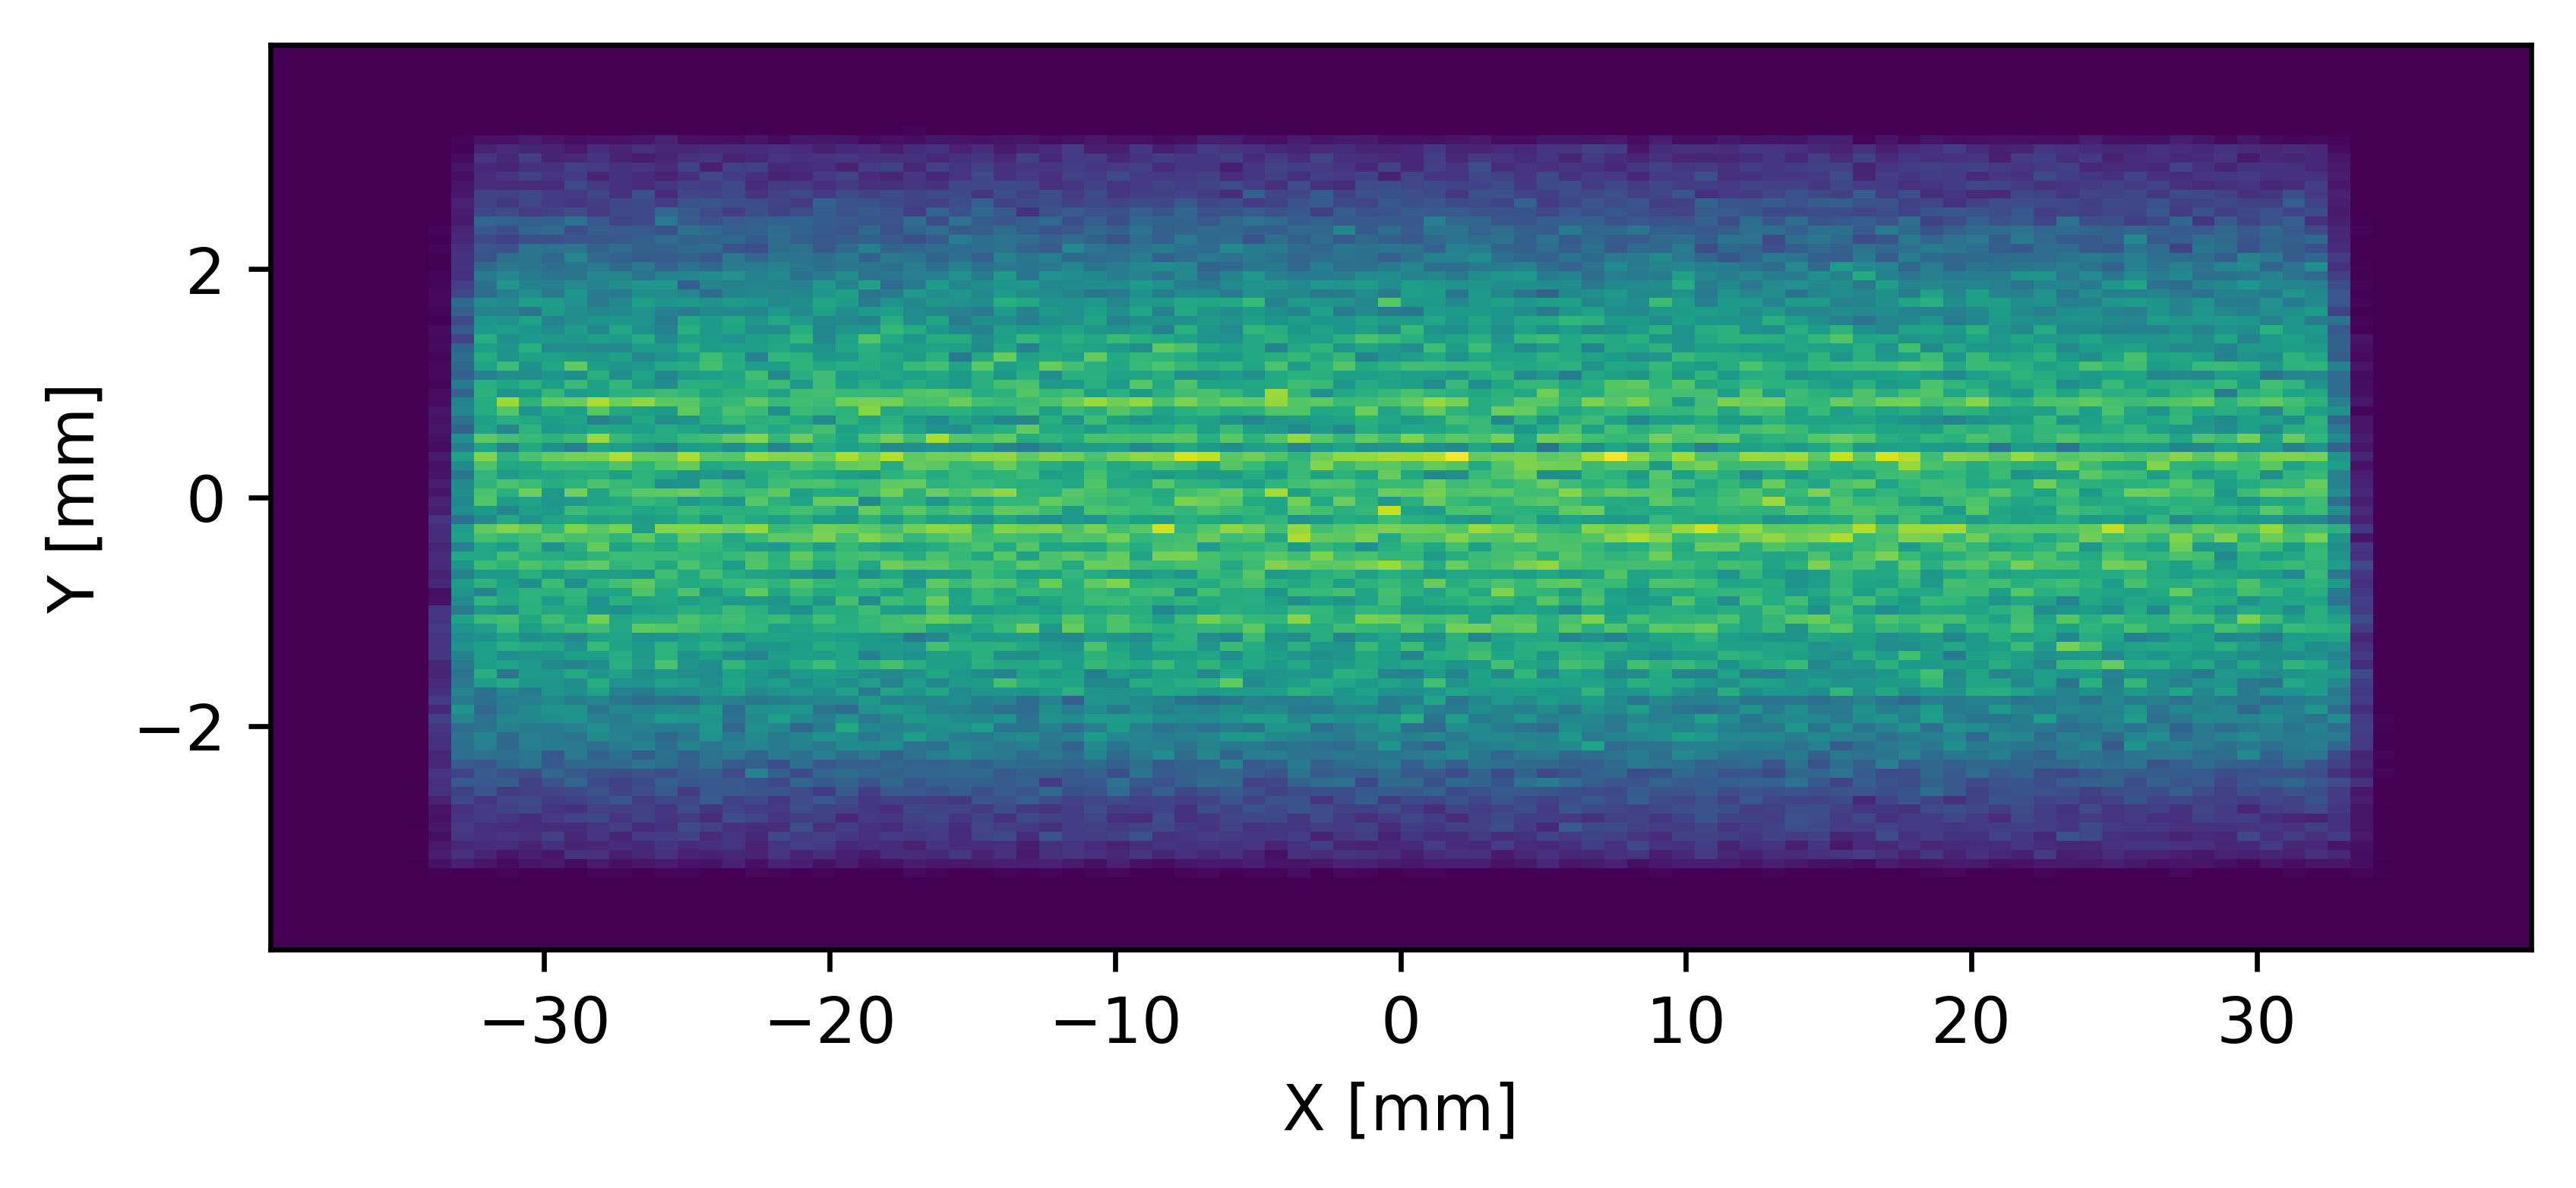
\includegraphics[width=0.85\linewidth]{./../figures/slope_error/WB4C_d30_d-spacing_gradient_45keV_slope_error01urad_ESRFID19PW150.png}
\end{figure}

\begin{figure}[H]
\centering
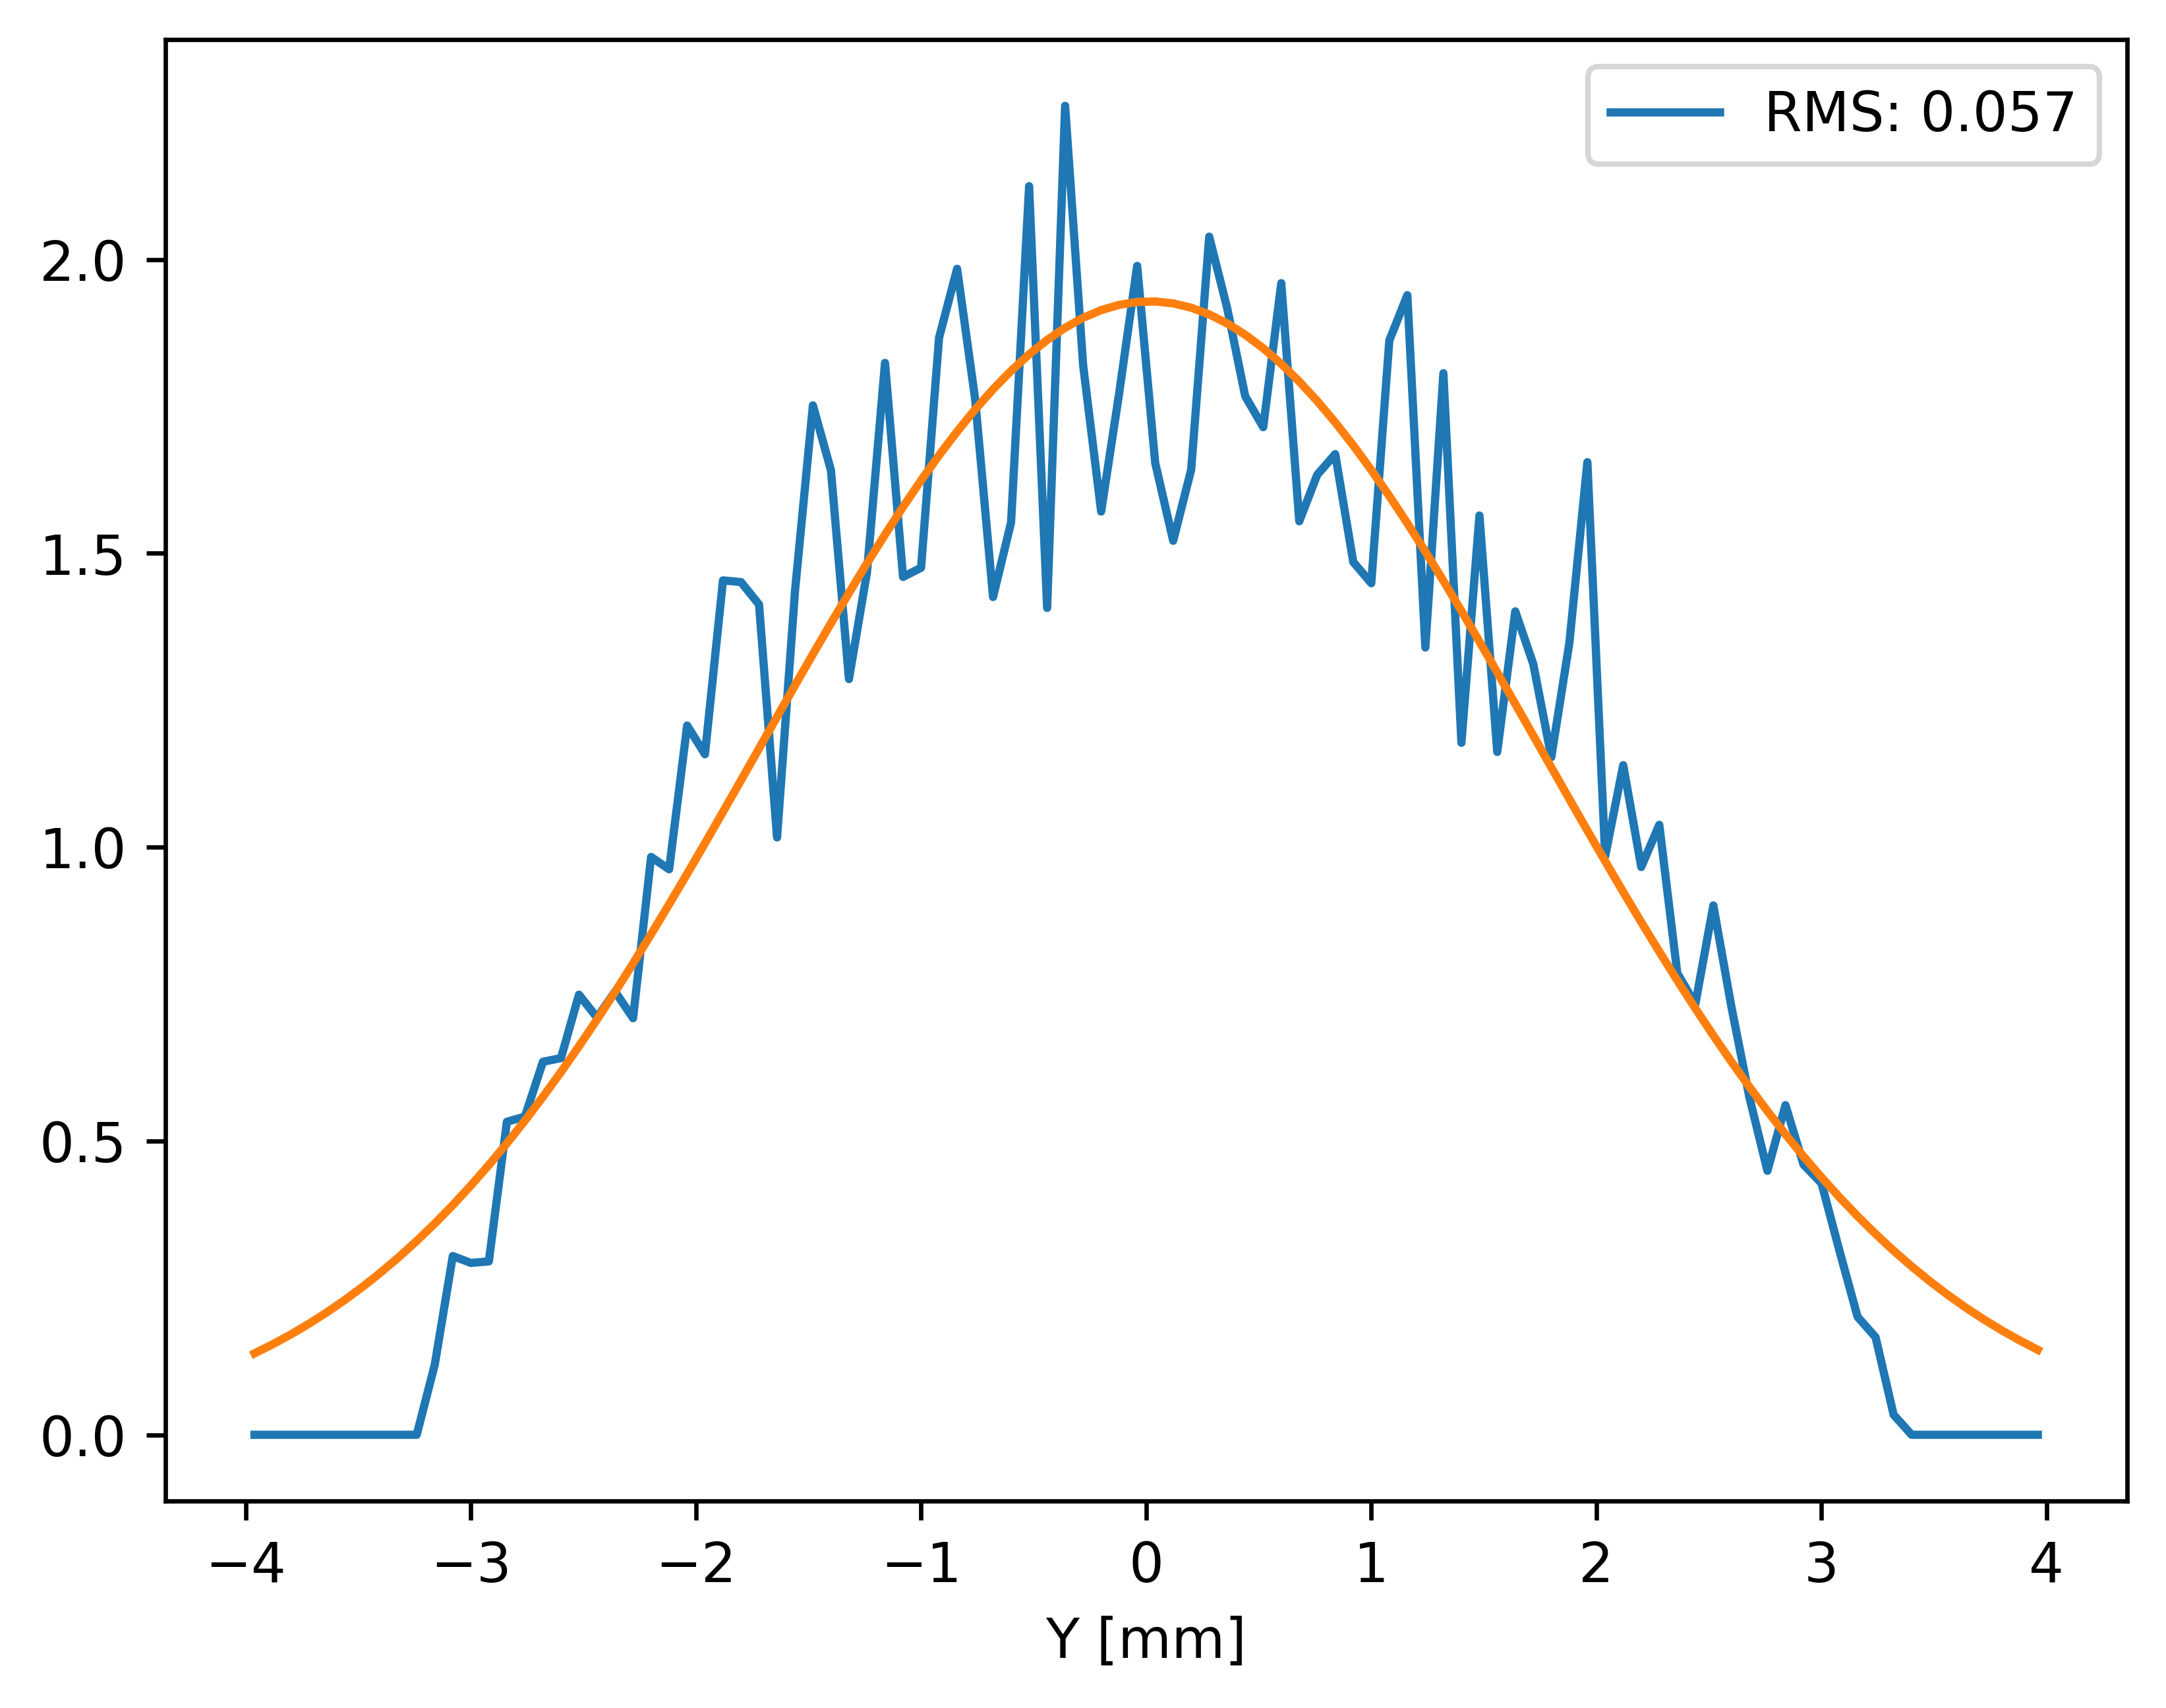
\includegraphics[width=0.85\linewidth]{./../figures/slope_error/WB4C_d30_d-spacing_gradient_45keV_slope_error01urad_ESRFID19PW150_Yprofile.png}
\caption{0.1 urad}
\label{fig:01urad}
\end{figure}

\clearpage
\subsubsection{0.2 urad}
\begin{figure}[H]
\centering
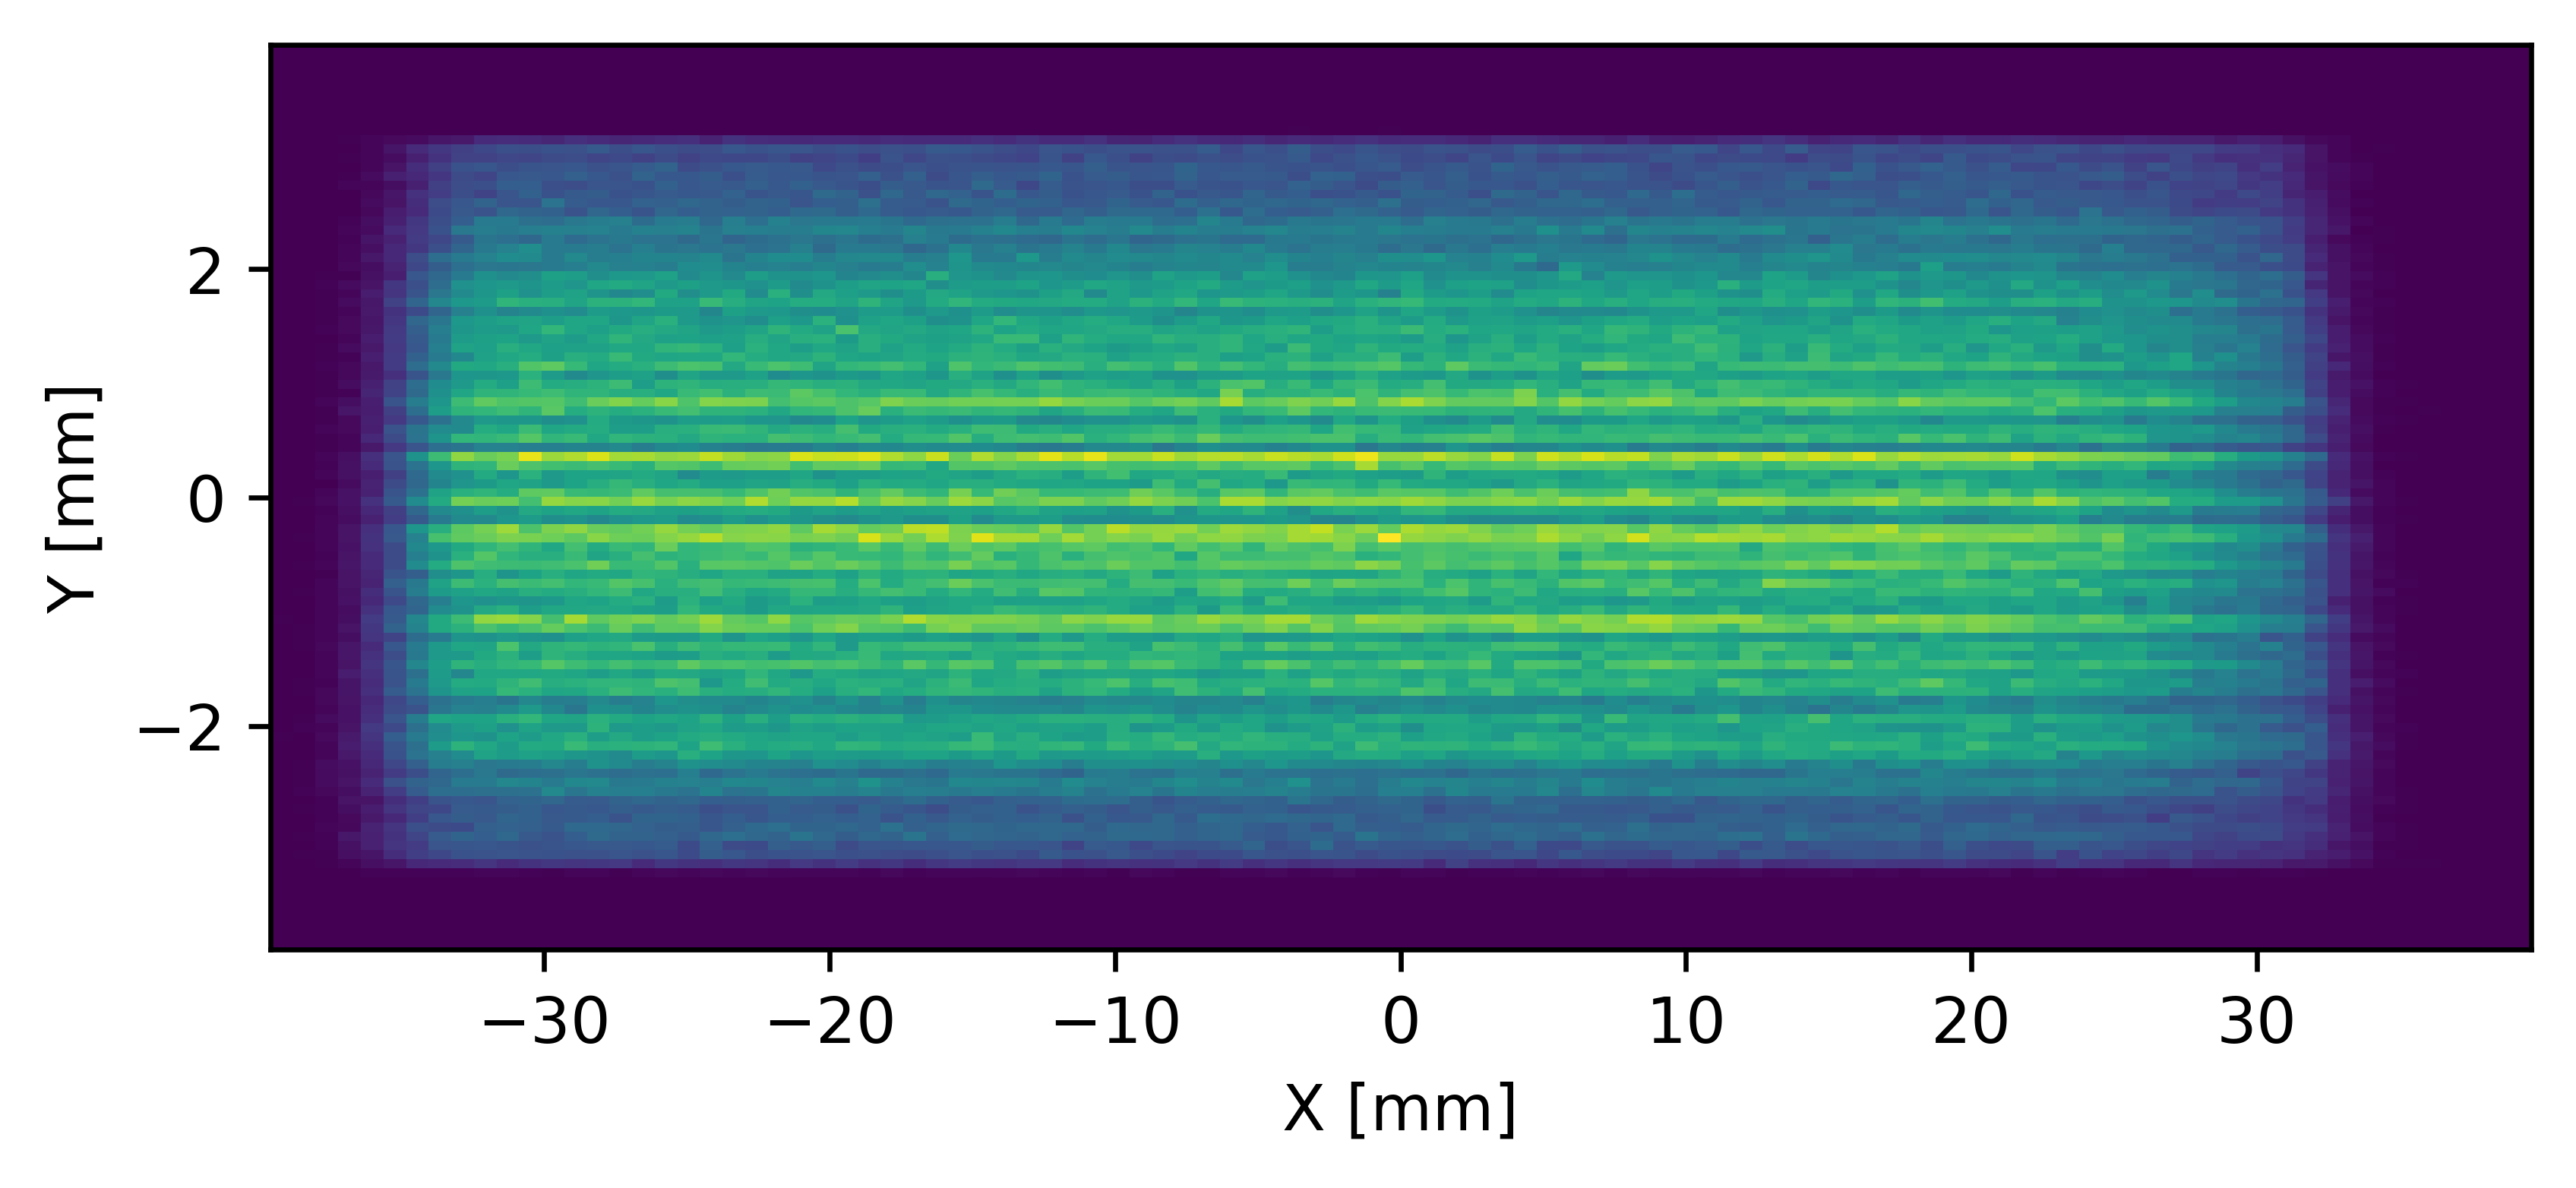
\includegraphics[width=0.9\linewidth]{./../figures/slope_error/WB4C_d30_d-spacing_gradient_45keV_slope_error02urad.png}
\end{figure}

\begin{figure}[H]
\centering
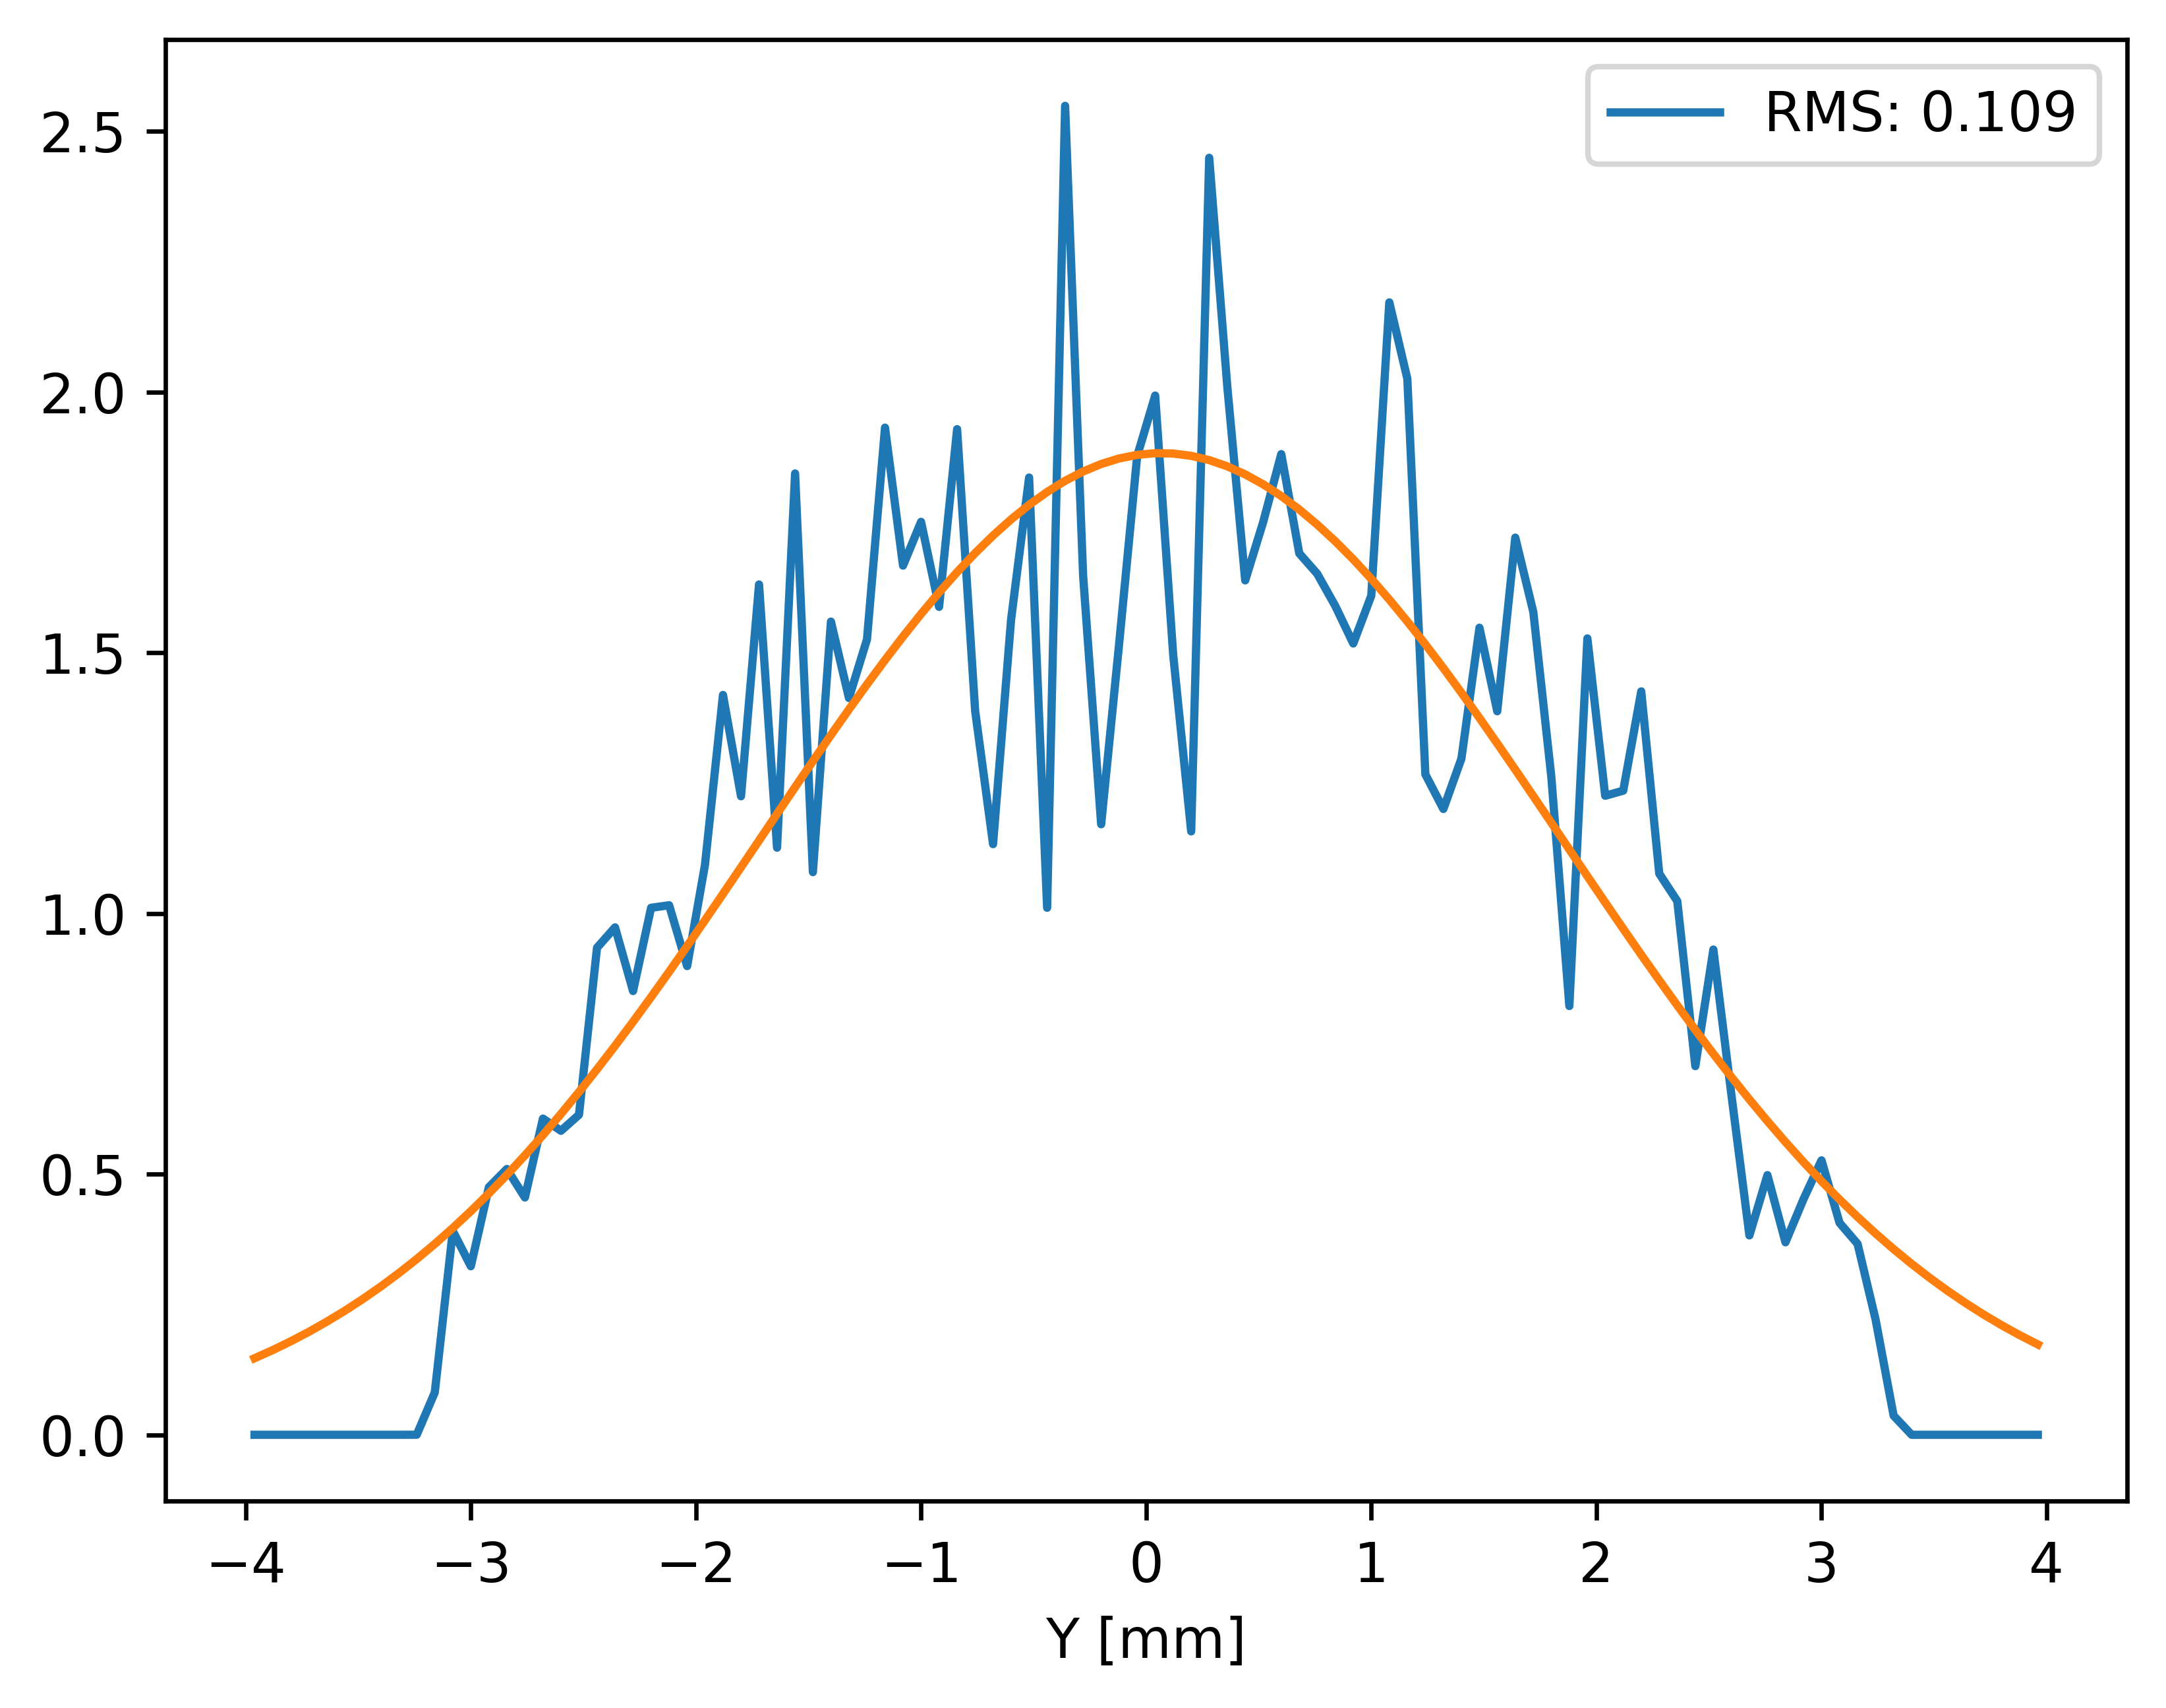
\includegraphics[width=0.9\linewidth]{./../figures/slope_error/WB4C_d30_d-spacing_gradient_45keV_slope_error02urad_ESRFID19PW150_Yprofile.png}
\caption{0.2 urad}
\label{fig:02urad}
\end{figure}

\clearpage
\subsubsection{0.3 urad}
\begin{figure}[H]
\centering
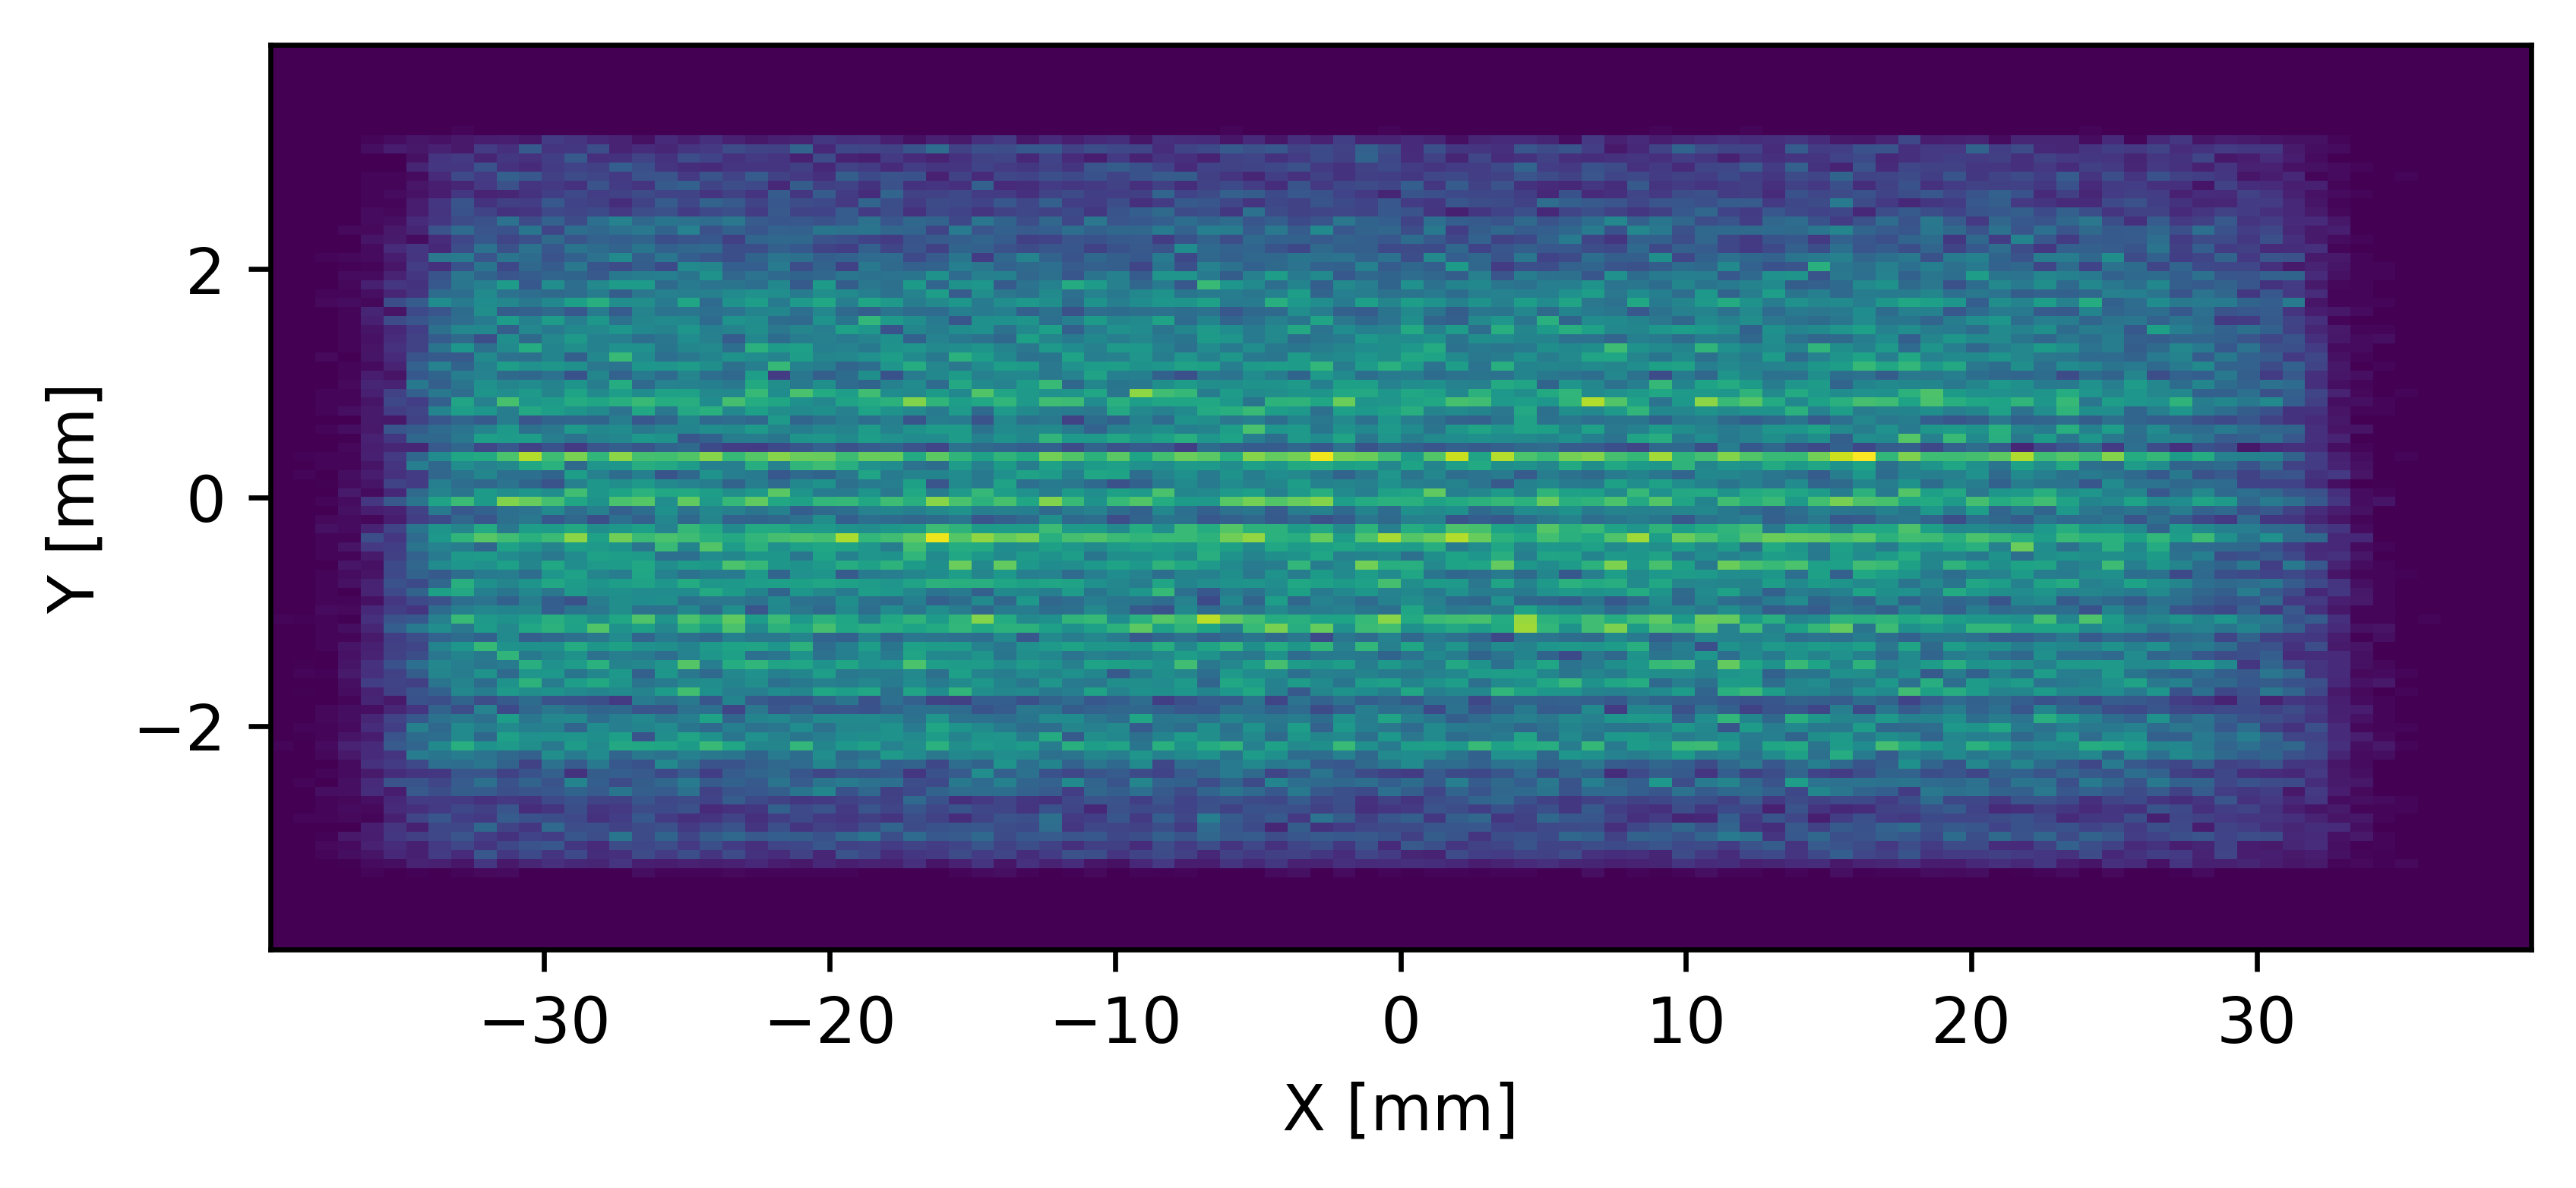
\includegraphics[width=0.9\linewidth]{./../figures/slope_error/WB4C_d30_d-spacing_gradient_45keV_slope_error03urad.png}
\end{figure}

\begin{figure}[H]
\centering
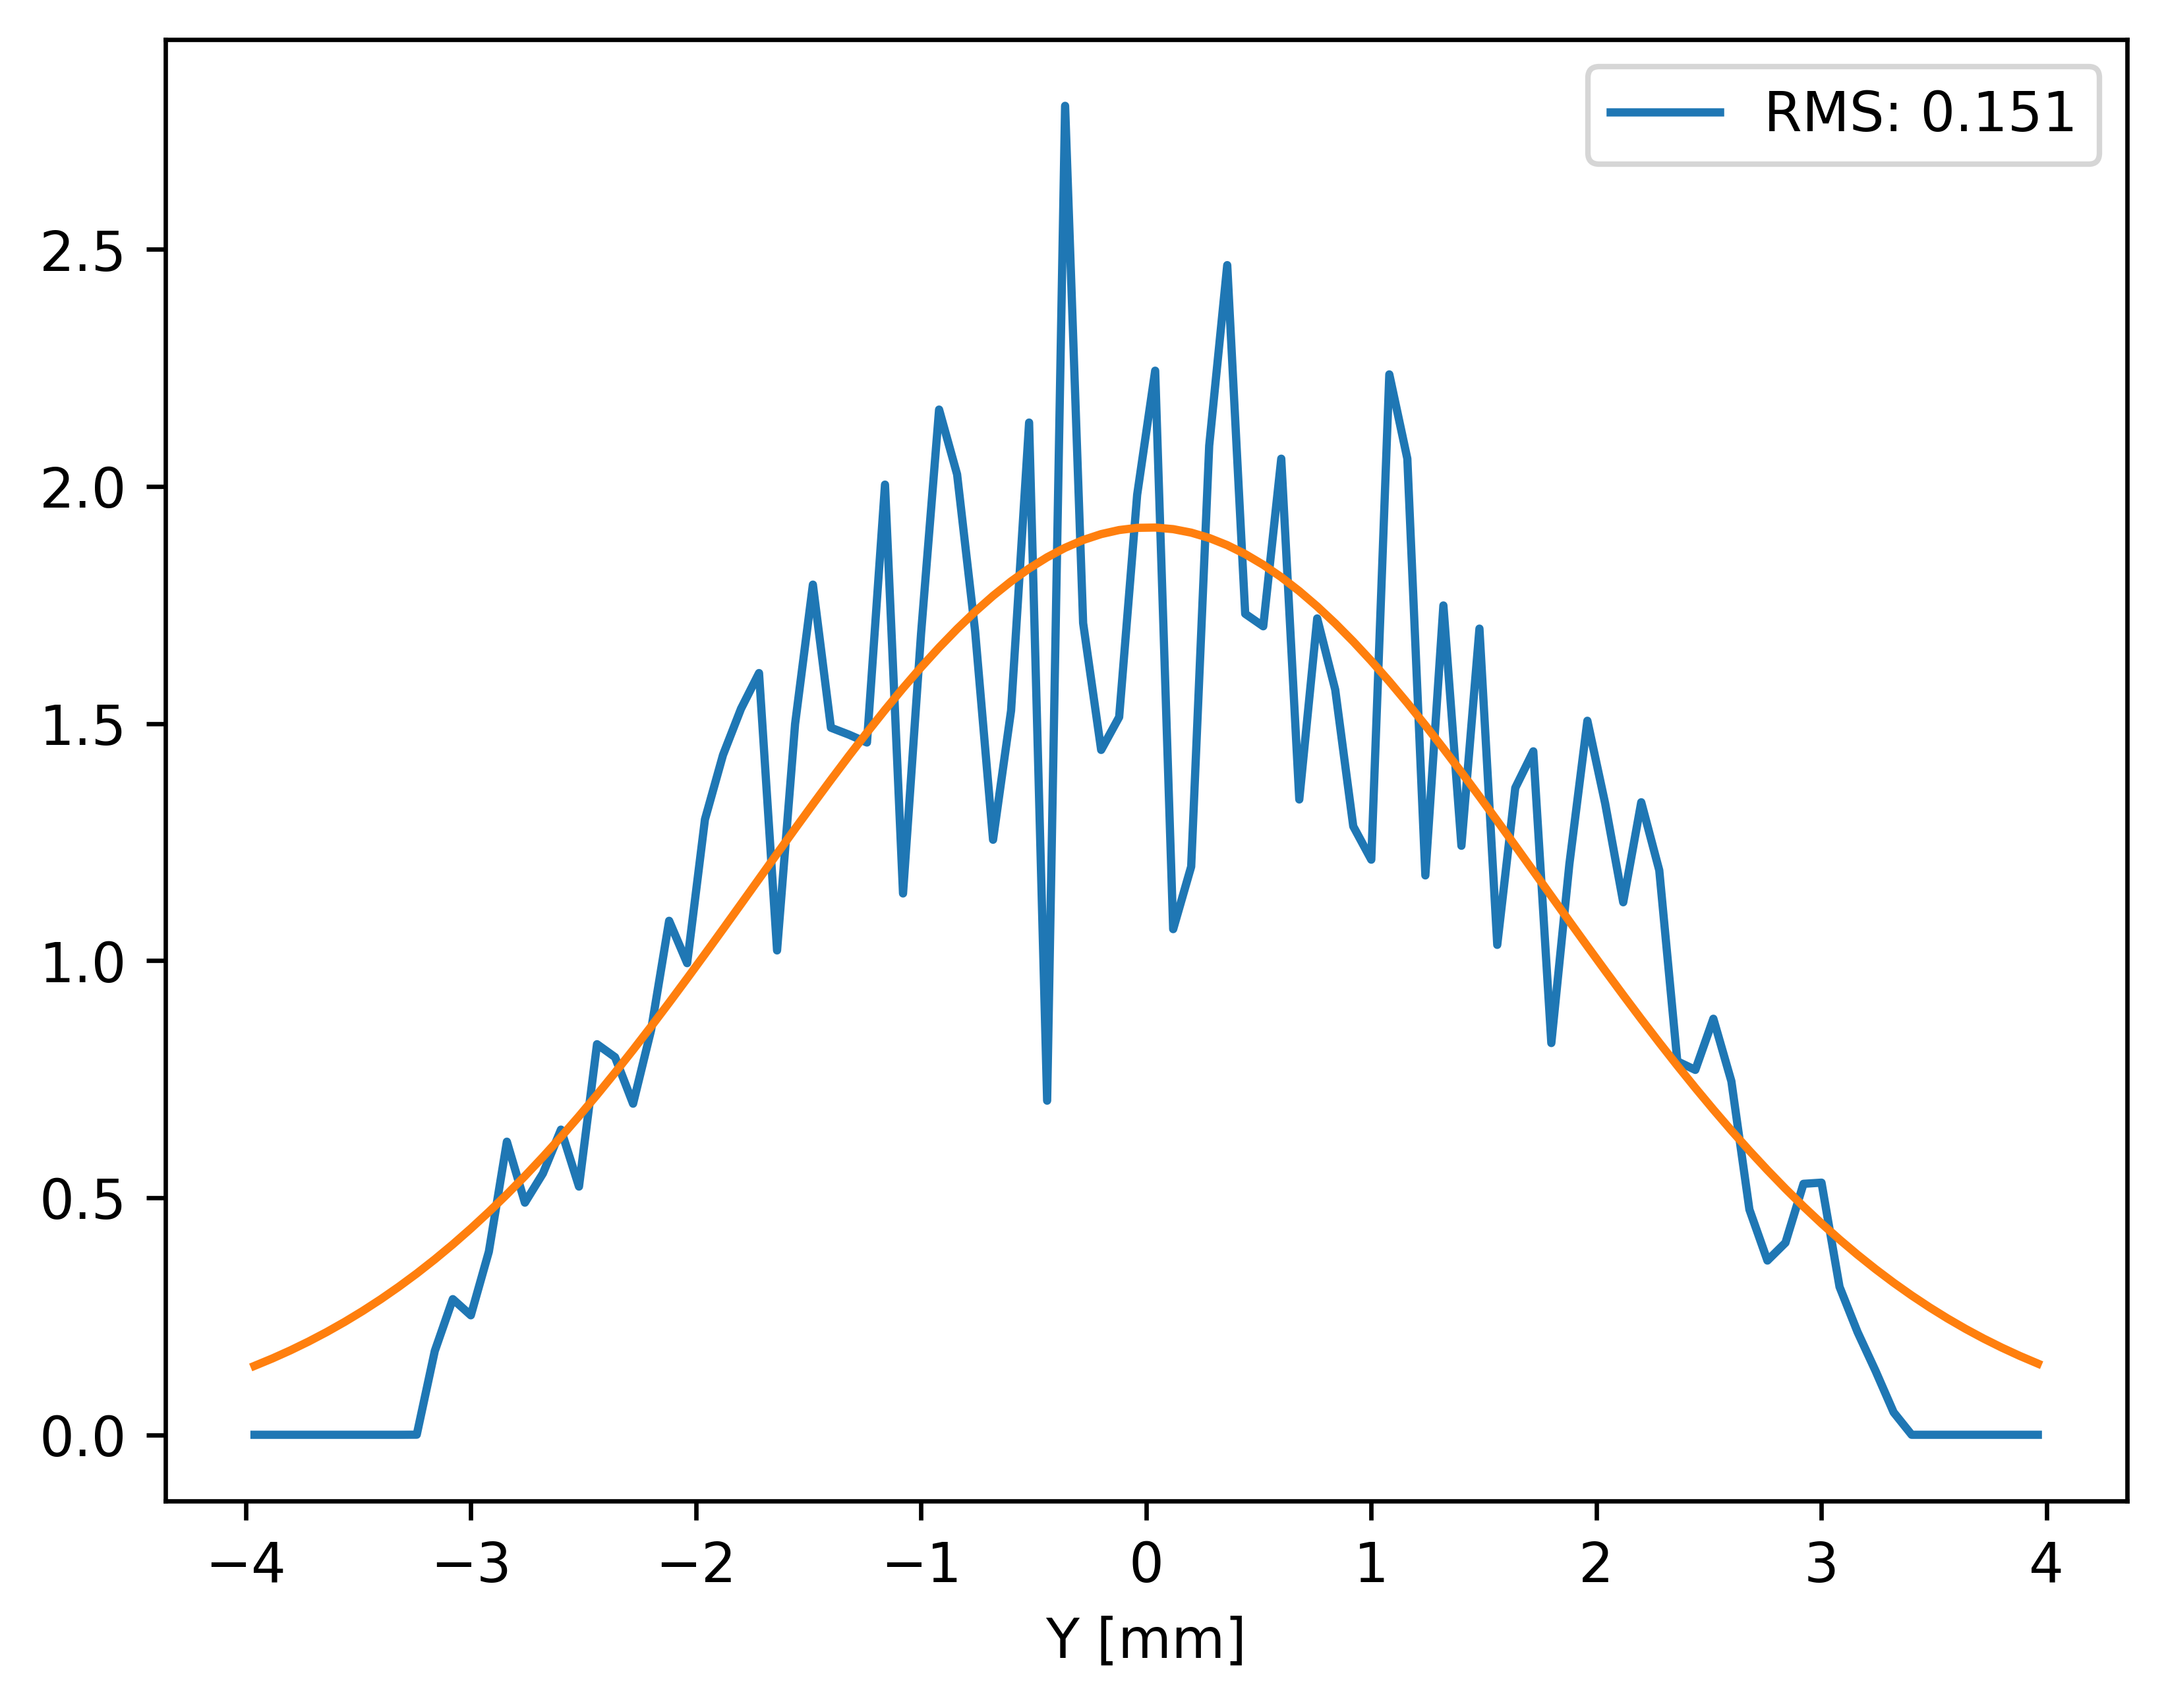
\includegraphics[width=0.9\linewidth]{./../figures/slope_error/WB4C_d30_d-spacing_gradient_45keV_slope_error03urad_ESRFID19PW150_Yprofile.png}
\caption{0.3 urad}
\label{fig:03urad}
\end{figure}

\clearpage
\subsubsection{0.4 urad}
\begin{figure}[H]
\centering
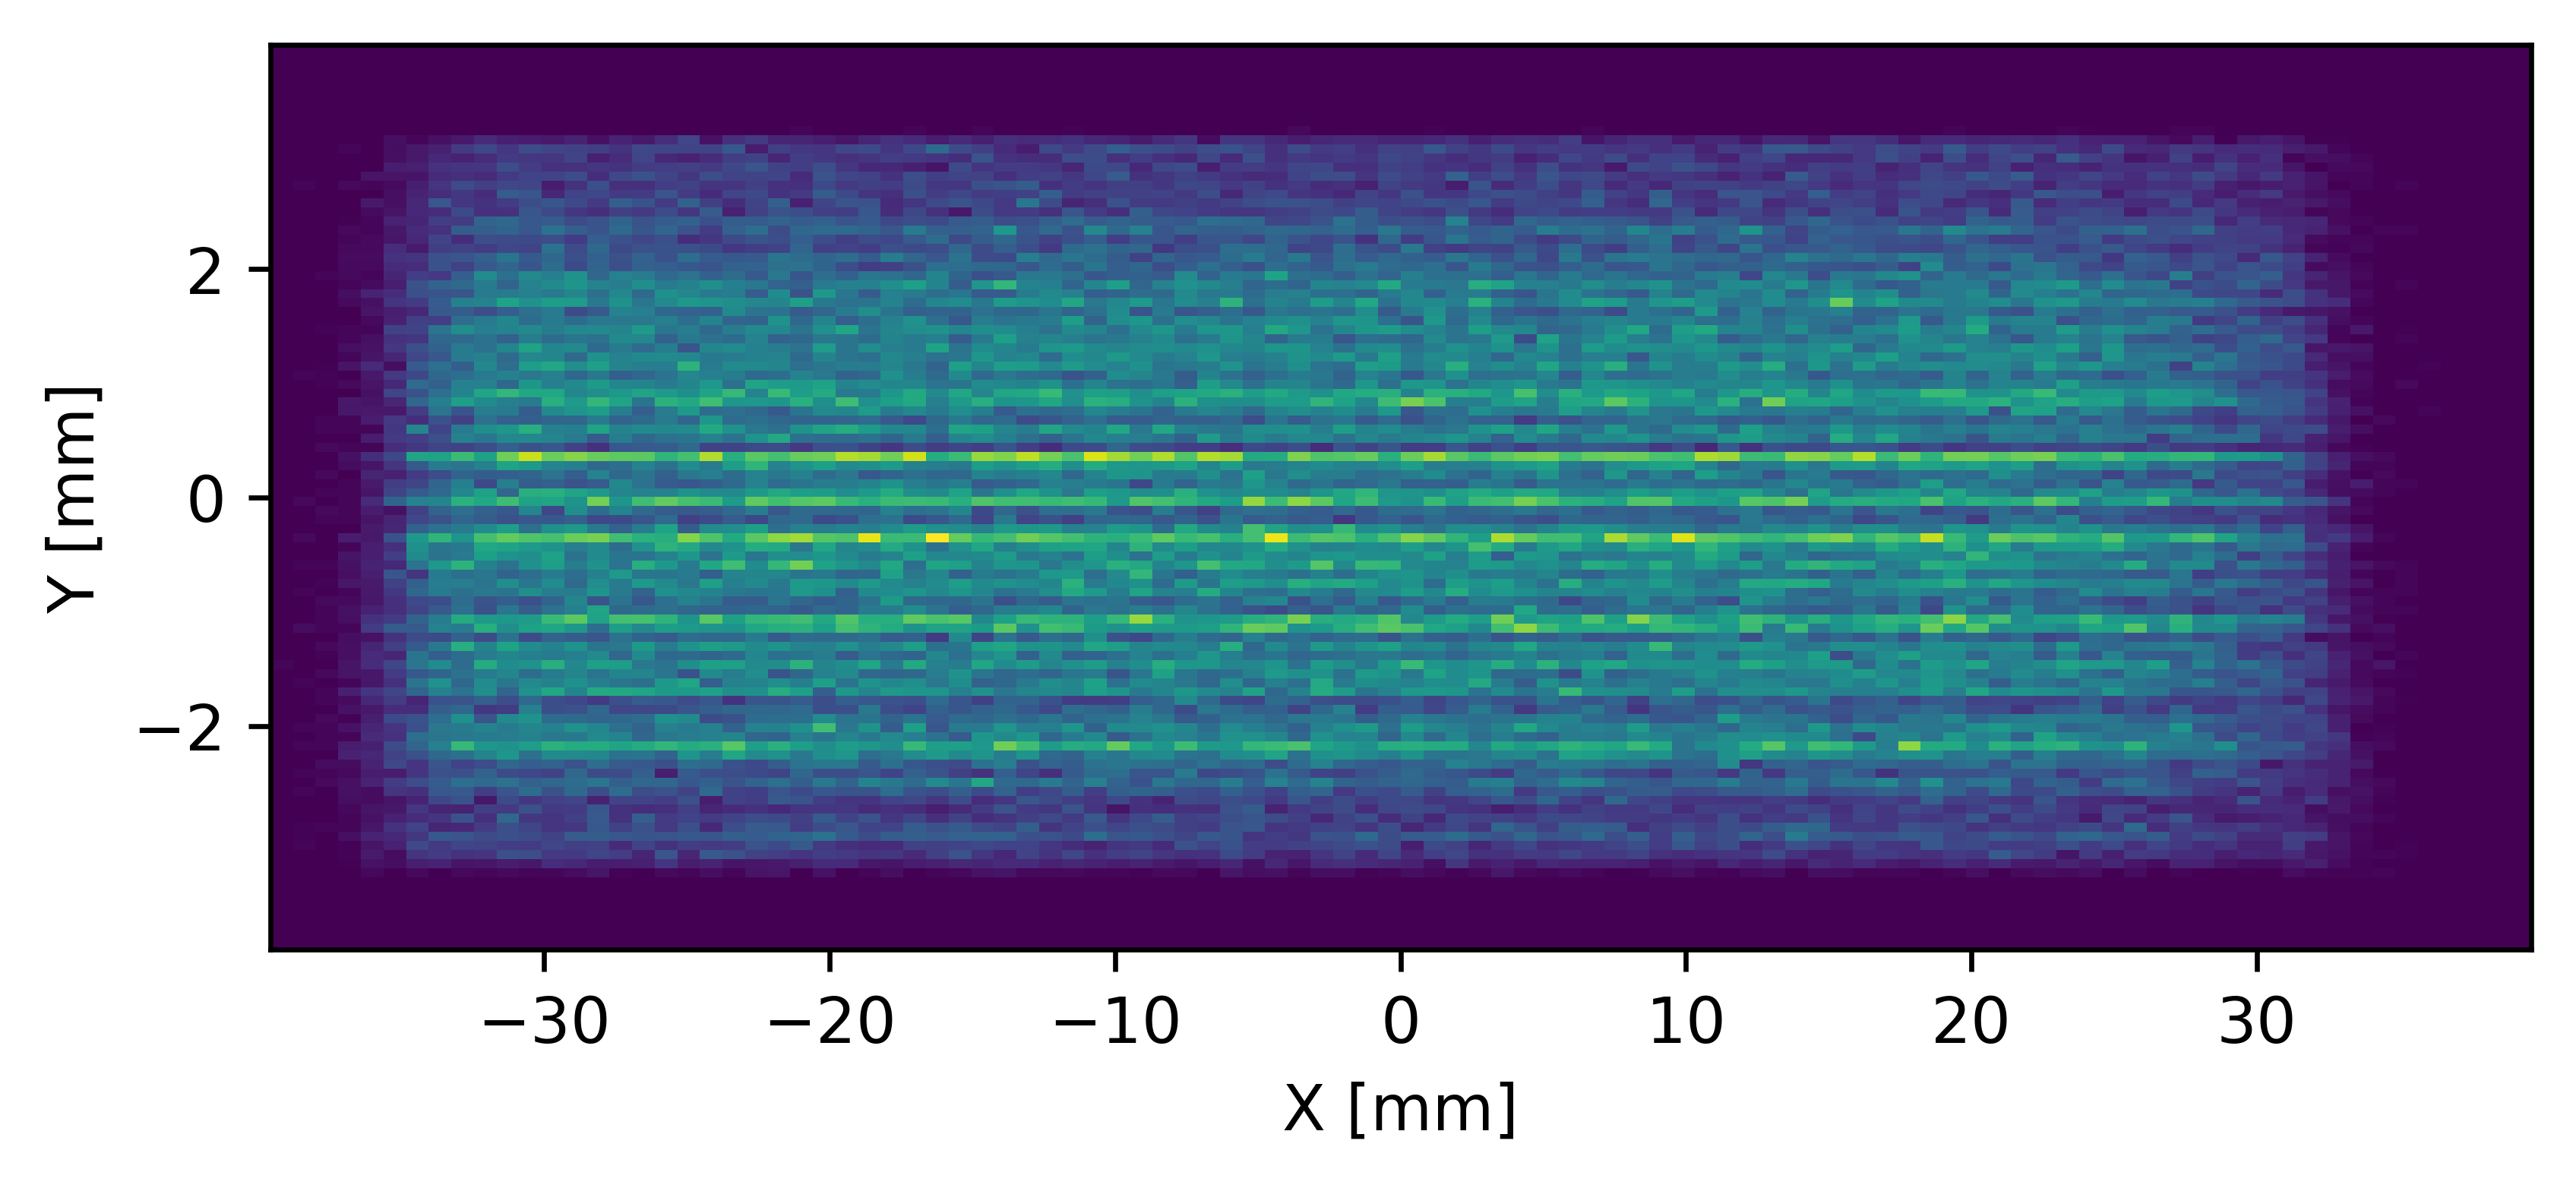
\includegraphics[width=0.9\linewidth]{./../figures/slope_error/WB4C_d30_d-spacing_gradient_45keV_slope_error04urad.png}
\end{figure}

\begin{figure}[H]
\centering
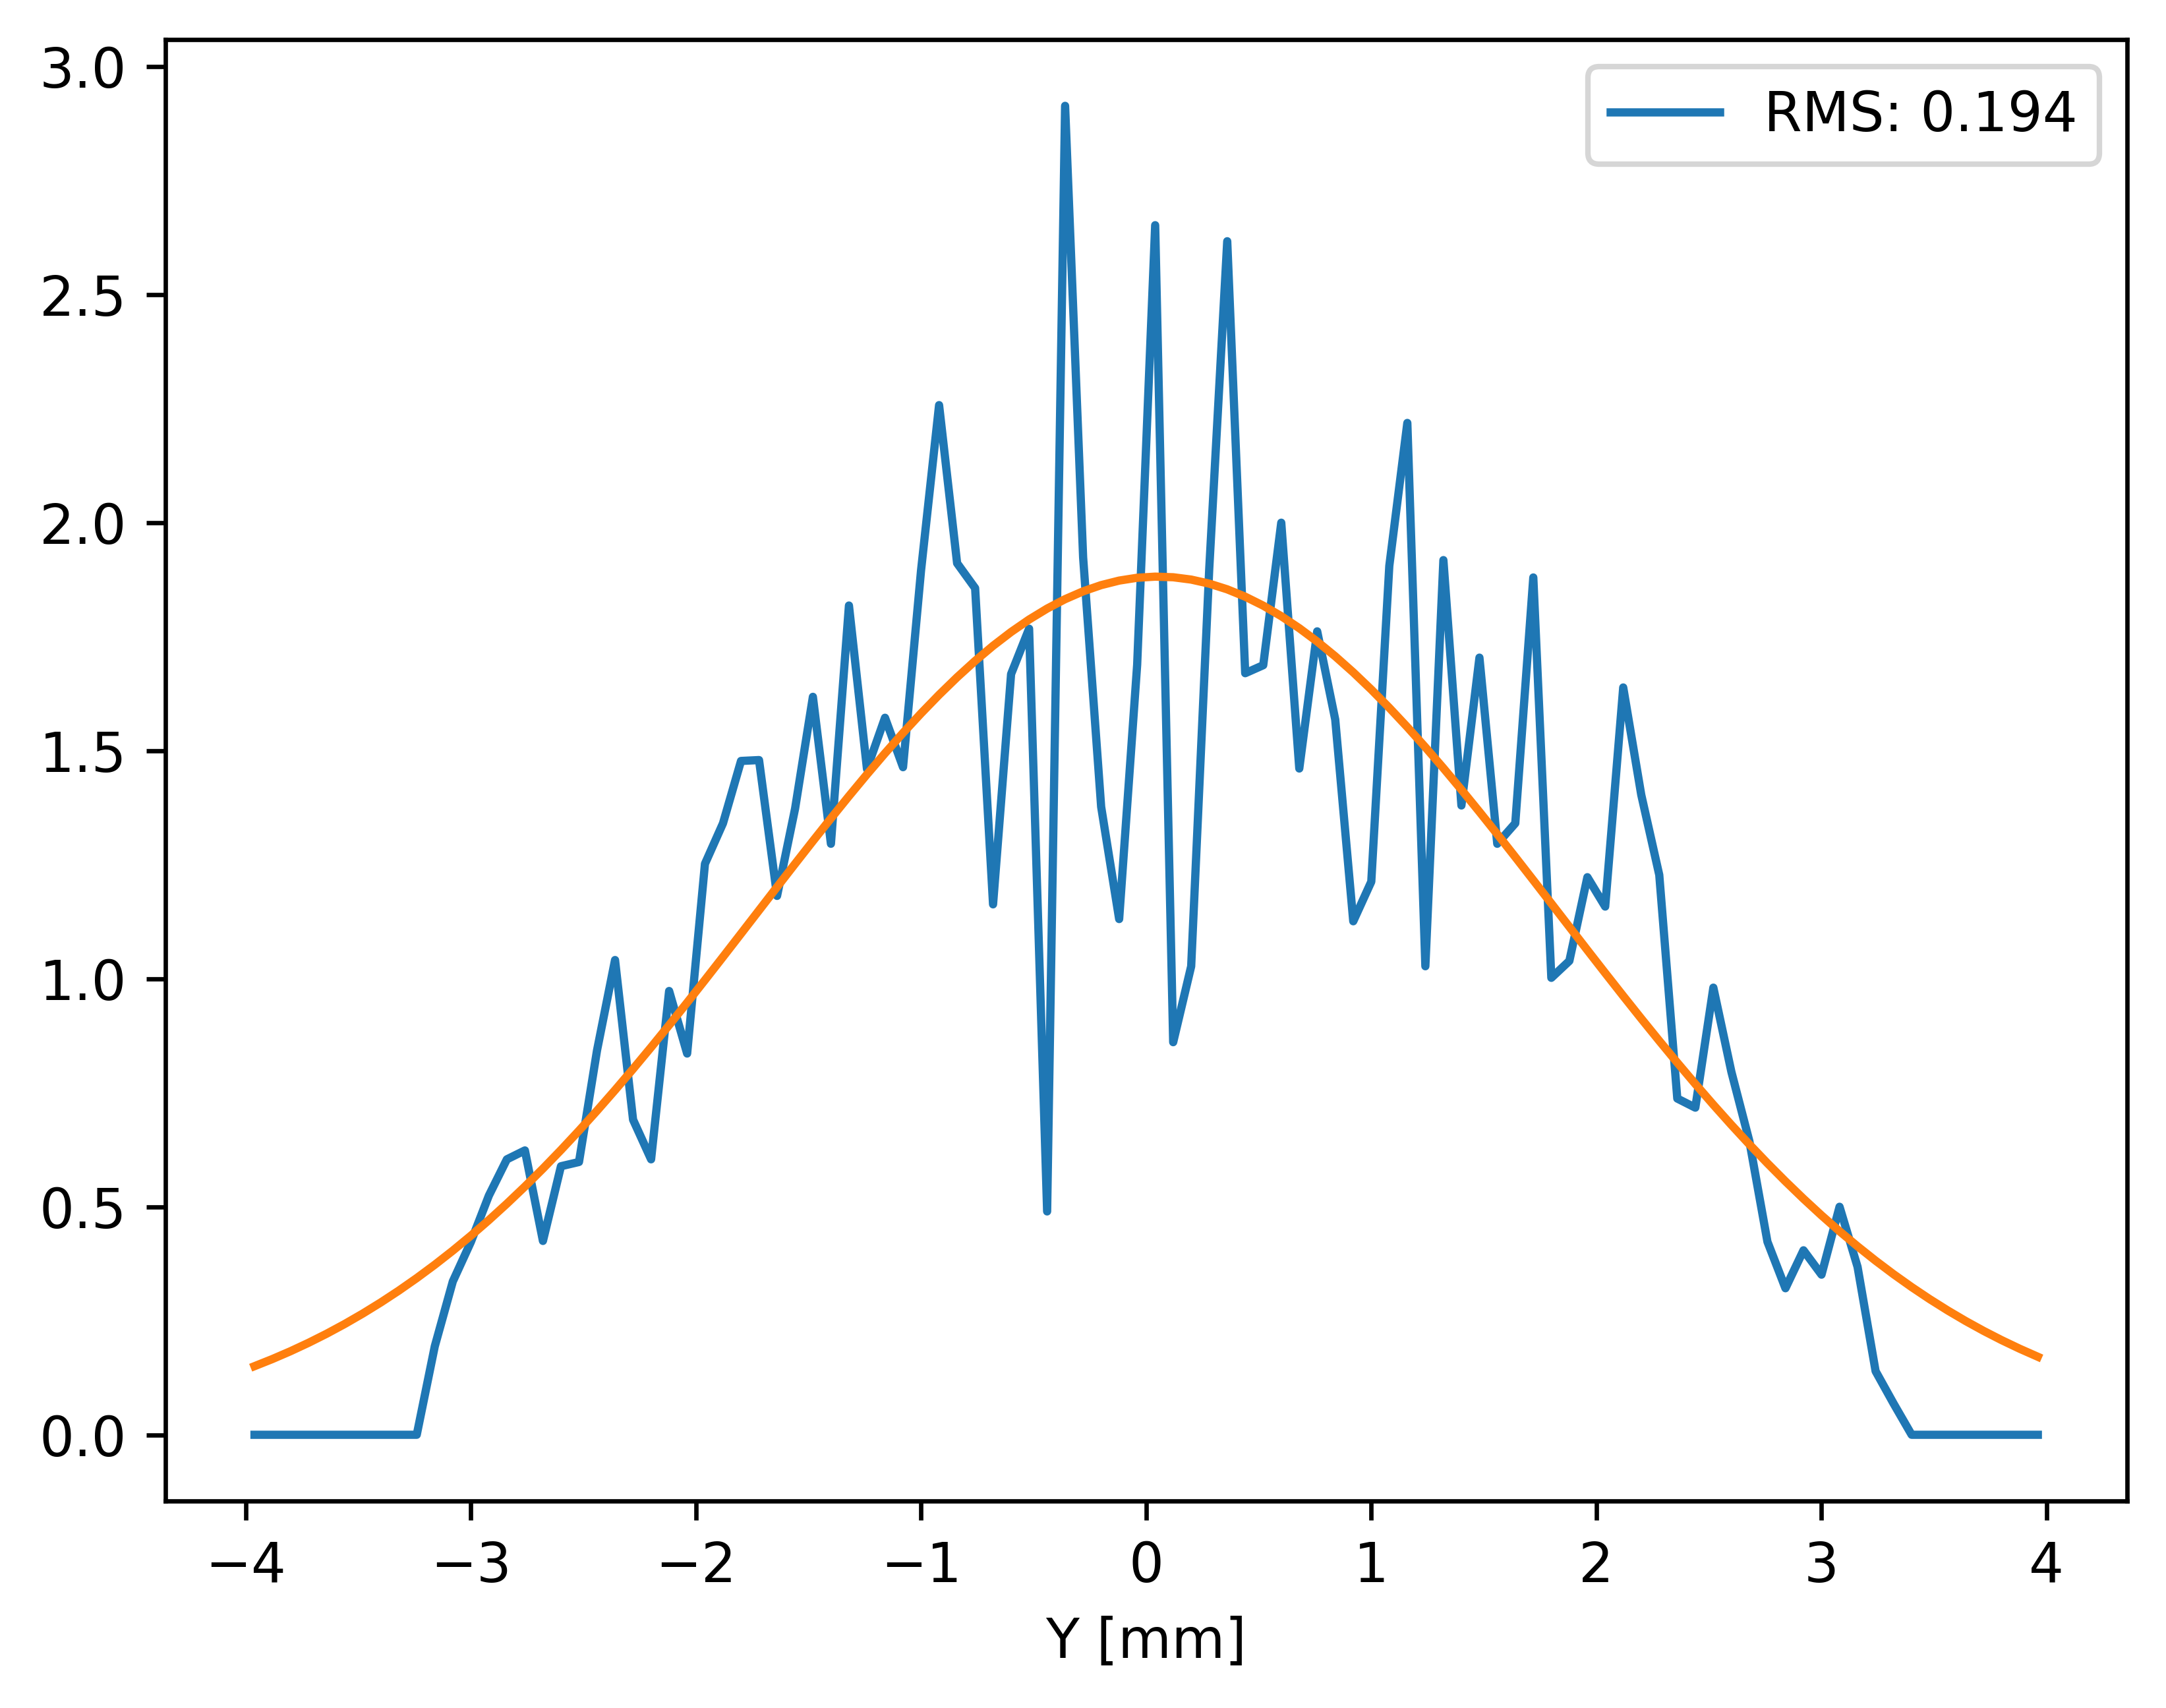
\includegraphics[width=0.9\linewidth]{./../figures/slope_error/WB4C_d30_d-spacing_gradient_45keV_slope_error04urad_ESRFID19PW150_Yprofile.png}
\caption{0.4 urad}
\label{fig:04urad}
\end{figure}

\clearpage
\subsubsection{0.5 urad}
\begin{figure}[H]
\centering
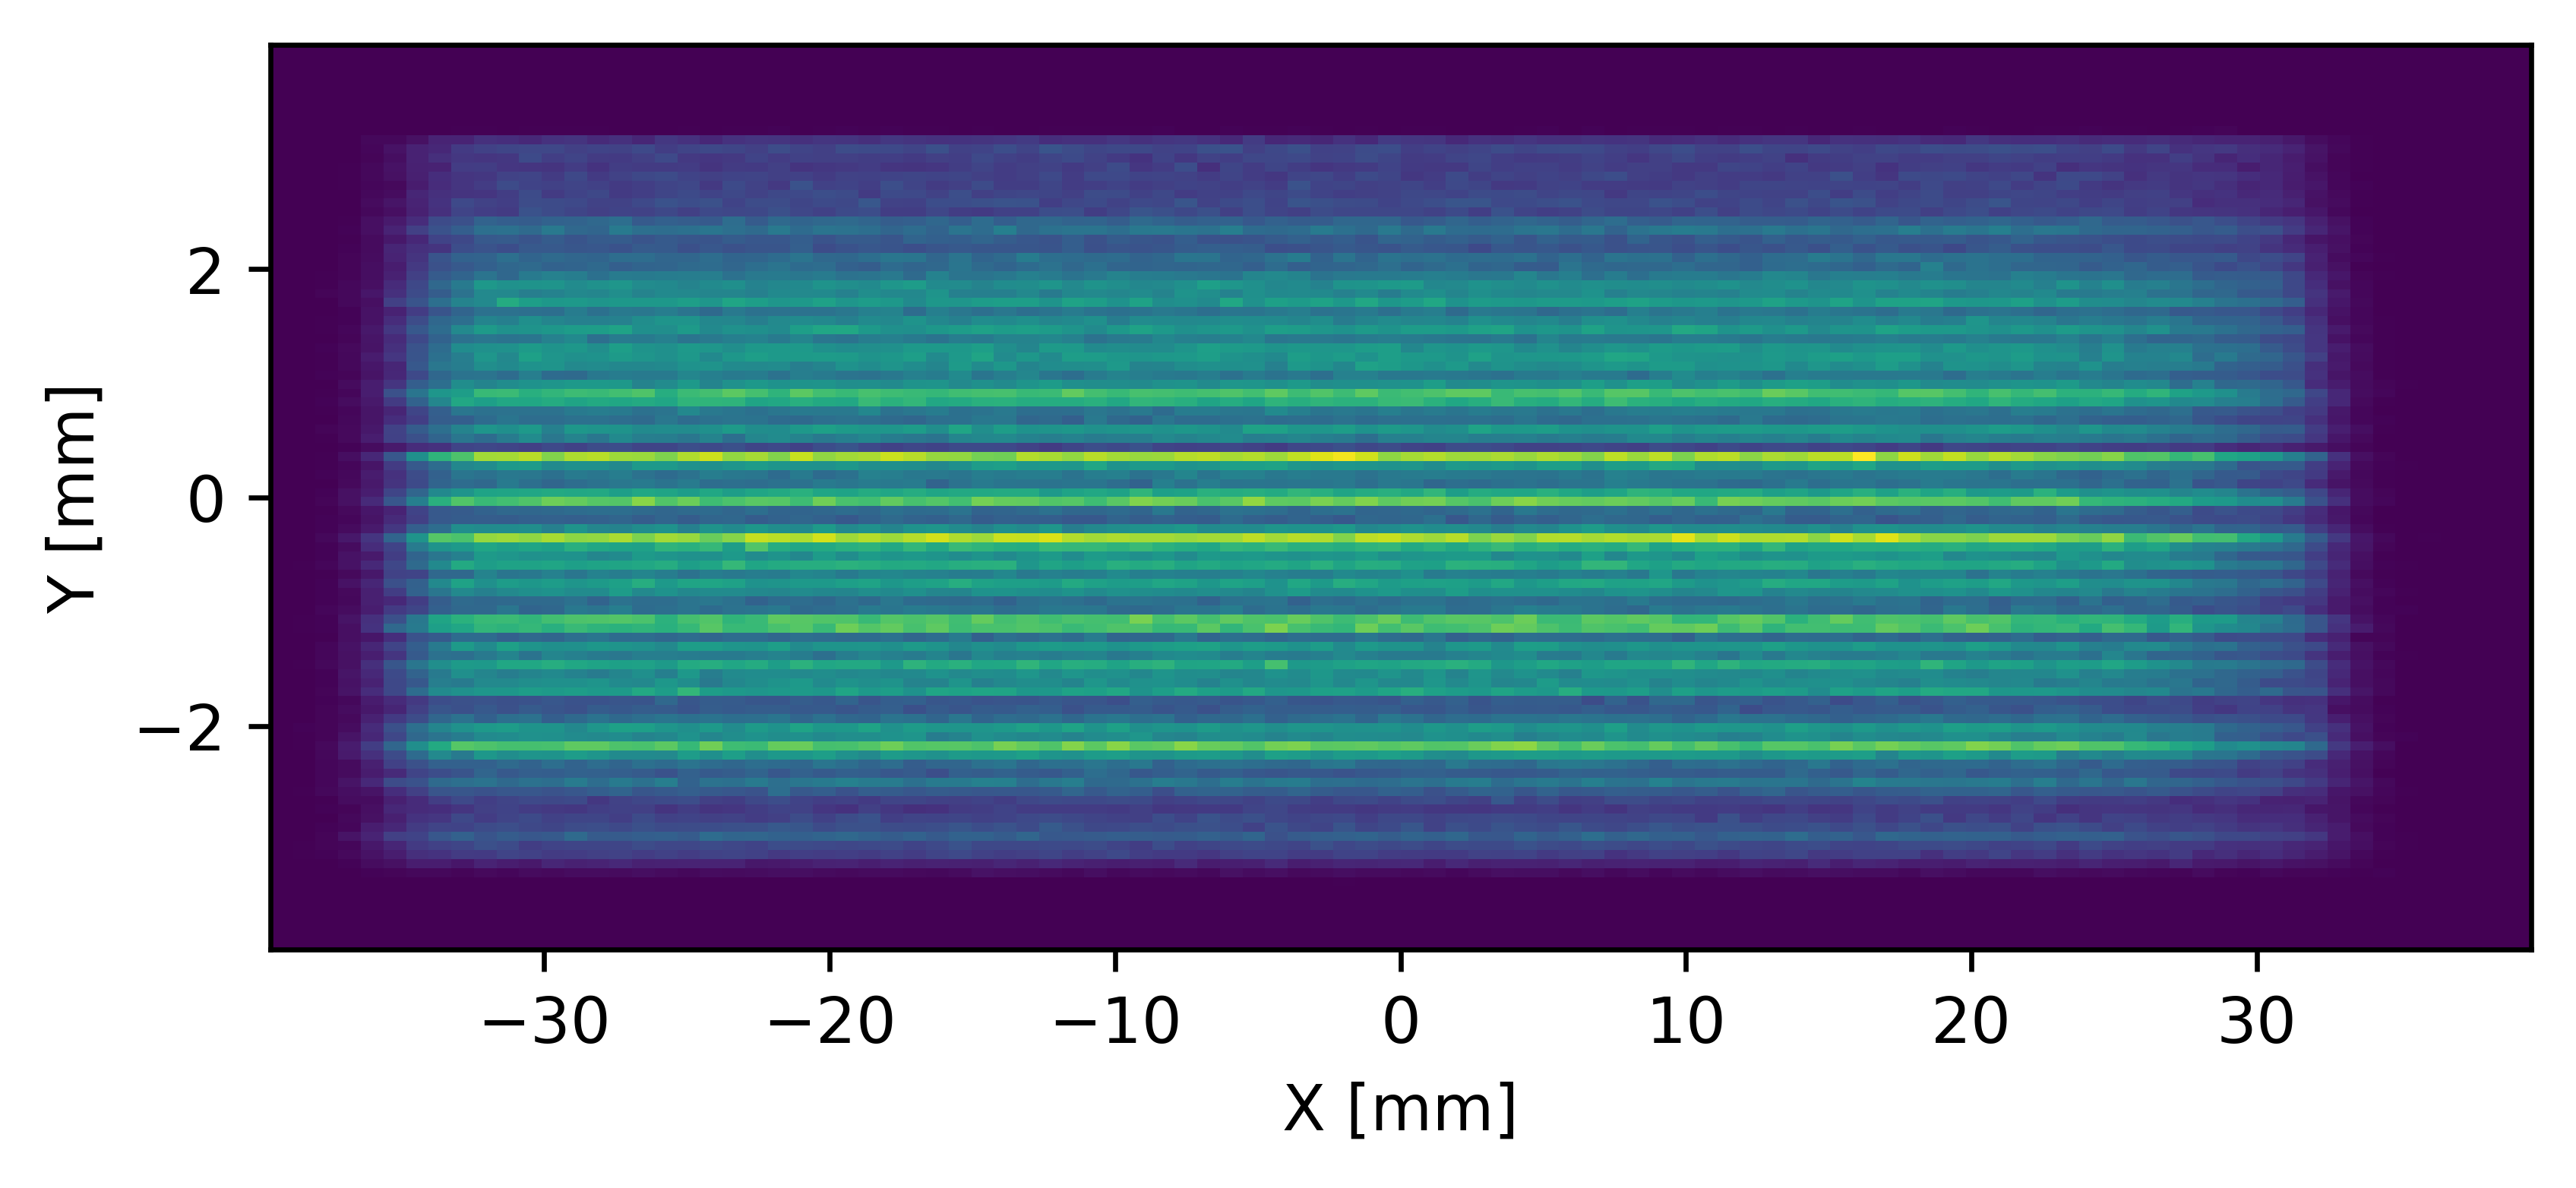
\includegraphics[width=0.9\linewidth]{./../figures/slope_error/WB4C_d30_d-spacing_gradient_45keV_slope_error05urad.png}
\end{figure}

\begin{figure}[H]
\centering
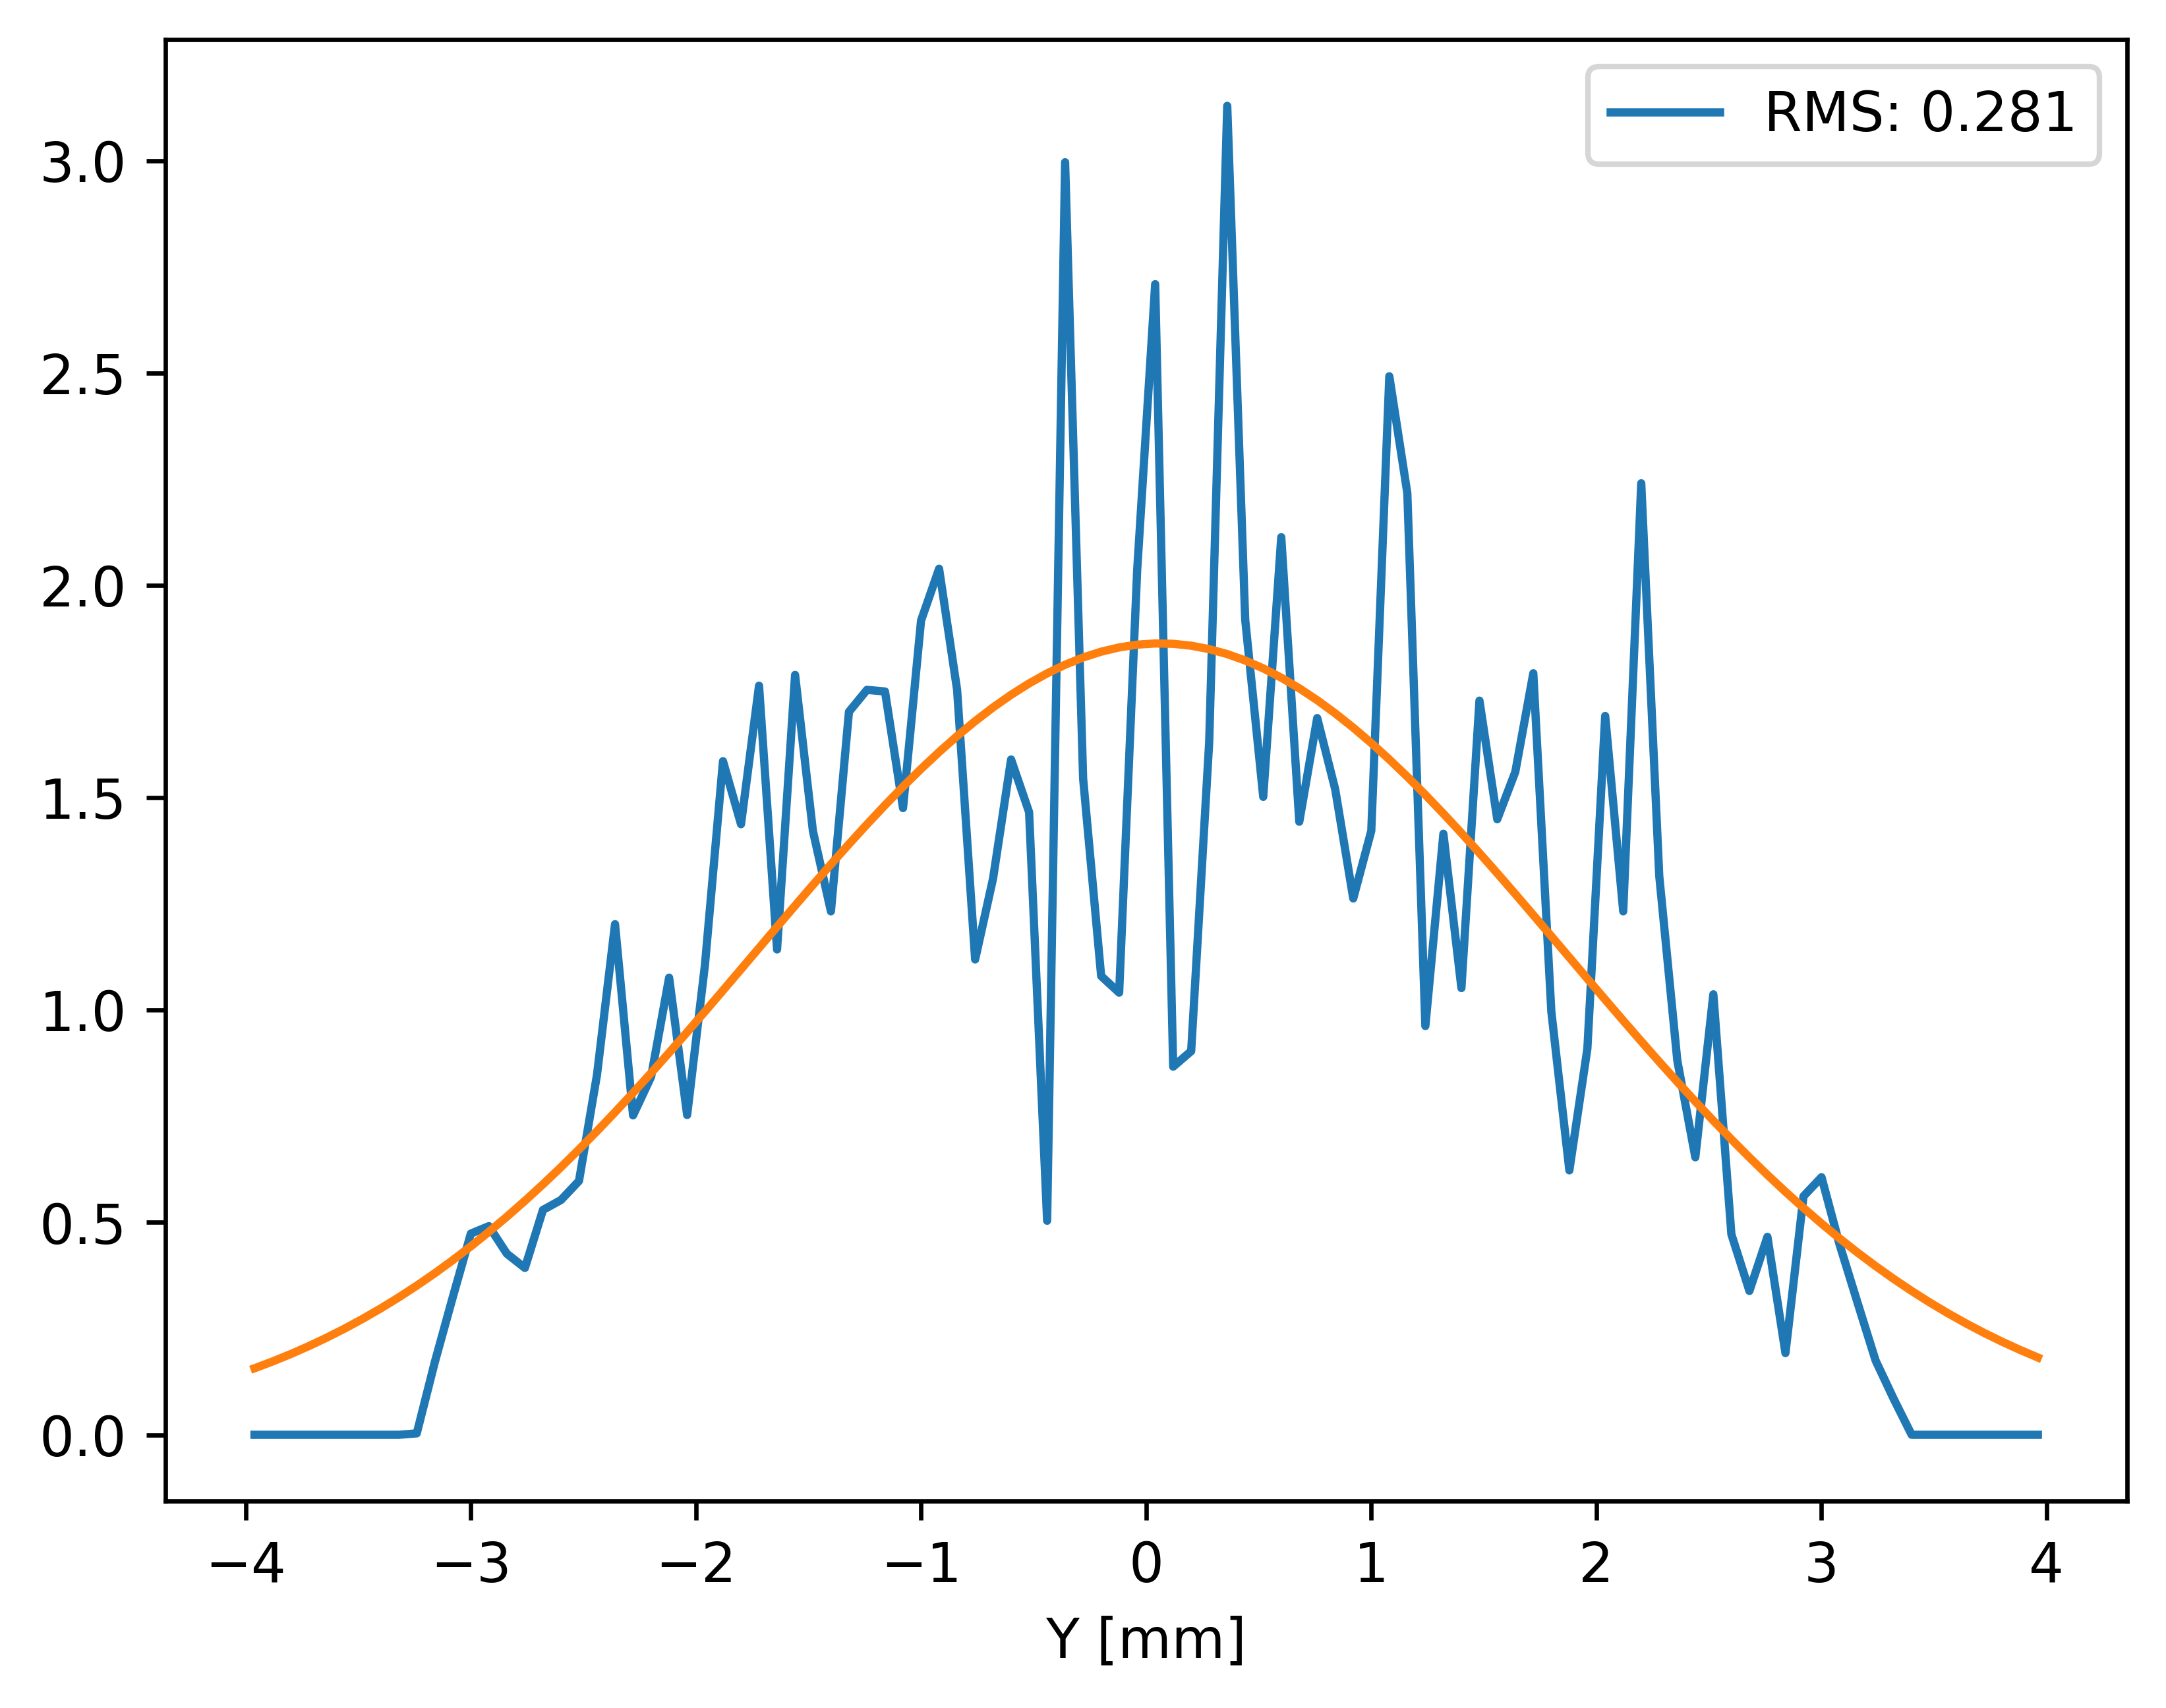
\includegraphics[width=0.9\linewidth]{./../figures/slope_error/WB4C_d30_d-spacing_gradient_45keV_slope_error05urad_ESRFID19PW150_Yprofile.png}
\caption{0.5 urad}
\label{fig:05urad}
\end{figure}


%%%%%%%%%%%%%%%%%%%%%%%%%%%%%%%%%%%%%%%%%%%%%%%%%%%%%%%%%%%%%%%%%%%%%%%%%%%%%%%%%%%%
\clearpage
\subsection{Thermal stability}
The thermal stability of ML1 should be verified with FEA simulations considering the white beam colliding with the mirror at the maximum Bragg angle allowed by the Bragg stage motorization (34.9 mrad). The thermal stability of the cooled mask in front of the ML1 profile shall be also verified.\\

The power density profile at 15.165 m from source is shown in Figure \ref{fig:power_profile_ML1}. Raw data can be found in the \powerprofilesurl. \\
\begin{figure}[ht]
\centering
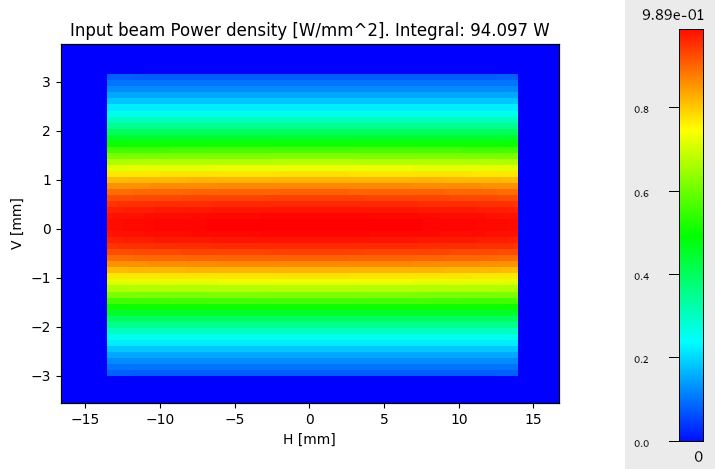
\includegraphics[width=0.8\textwidth]{./../../power_profiles/power_profile_ML1.png}
\caption{\label{fig:power_profile_ML1} Power density profile at 15.165 m from source (center position of ML1).}
\end{figure}